\documentclass[10pt]{book}
\usepackage[utf8]{inputenc}
\usepackage[italian]{babel}
\usepackage{multicol}
\usepackage[bookmarks]{hyperref}
\usepackage[a4paper, total={18cm, 25cm}]{geometry}
\usepackage{listings}
\usepackage{color}
\definecolor{gray}{rgb}{0.5,0.5,0.5}
\lstset{
	language=C,
	commentstyle=\itshape\color{gray},
	morekeywords={output}
}
\usepackage{graphicx}
\usepackage{makecell}
\graphicspath{ {./img/} }
\usepackage{color}

\begin{document}
\renewcommand*\contentsname{Indice}
\title{Crittografia}
\author{Federico Matteoni}
\date{A.A. 2020/21}
\maketitle
\tableofcontents
\pagebreak
\section*{Introduzione}
Prof.ssa: Anna Bernasconi.\\
Vedremo i cifrari da un punto di vista prettamente algoritmico. Vedremo anche i cifrari storici, ormai non più utilizzabili, perché hanno "aperto la strada", per poi passare ai cifrari perfetti (soluzione ideale ma con costo elevato).\\
Poi esamineremo i cifrari simmetrici, a chiave pubblica, curve ellittiche, firma digitale, SSL. Protocolli zero knowledge, blockchain e crittografia quantistica.\\\\
Libro di testo: Bernasconi, Ferragina, Luccio - Elementi di Crittografia.
\paragraph{Esame} Orali nel caso di esami a distanza, scritto nel caso di esami in presenza, closed-book.
\chapter{Introduzione alla Crittografia}
\section{Introduzione}
\paragraph{Crittografia} Significa "\textit{scrittura nascosta}", si intendono tecniche matematiche per mascherare i messaggi per non renderli leggibili a terzi (\textbf{crittografia}) o tentare di svelarli quando non si è il legittimo destinatario (\textbf{crittoanalisi}). Quindi tecniche di protezione e viceversa.\\
Esiste per i due mondi in contrapposizione: persone che vogliono scambiarsi privatamente informazioni e gli \textit{impiccioni} che desiderano ascoltare o intromettersi nelle conversazioni altrui (per curiosità, investigazione o altri scopi).
\paragraph{Due gruppi di persone} Chi vuole proteggersi userà \textbf{metodi di cifratura}, gli altri useranno \textbf{metodi di crittoanalisi}
\subparagraph{Crittografia} Metodi di Cifratura
\subparagraph{Crittoanalisi} Metodi di \ldots
\textbf{crittologia} studio comunicazione canali non sicuri e relativi problemi
\subsection{Lo scenario}
Alice vuole comunicare con Bob su un canale insicuro, quindi adottano un metodo di cifratura per spedire il messaggio in chiaro \texttt{m} sottoforma di crittogramma \texttt{c} (testo cifrato) che deve essere: incomprensibile al crittoanalista Eve (eavesdropper) in ascolto sul canale, ma facilmente decifrabile da Bob.
\paragraph{MSG} Insieme dei messaggi in chiaro
\paragraph{CRITTO} Insieme dei crittogrammi
\begin{center}
C : MSG $\rightarrow$ CRITTO\\
D : CRITTO $\rightarrow$ MSG
\end{center}
Sono operazioni da poter fare in tempo polinomiale. 
C e D sono una l'inversa dell'altra, ma C \textbf{deve essere iniettiva}.
\begin{center}
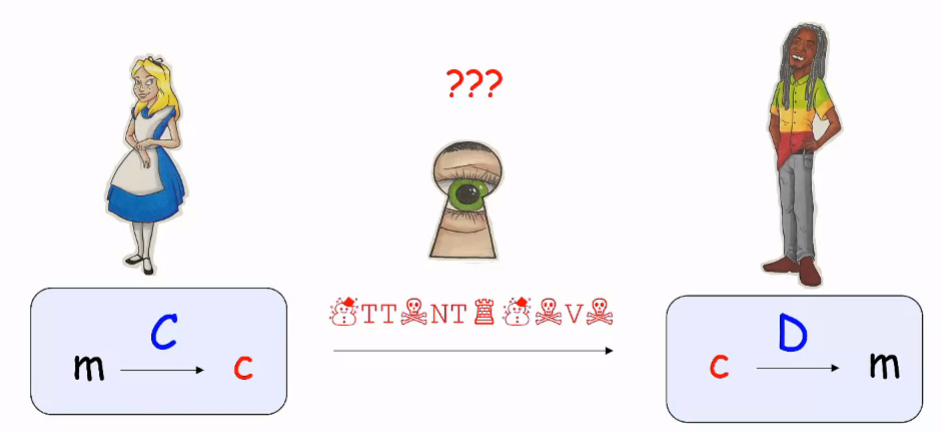
\includegraphics[scale=0.55]{1.png}
\end{center}
\subsection{Antichi esempi}
\paragraph{Erodoto} Nelle \textit{Storie}, V secolo a.C.\\
Messaggi tatuati sulla testa, coperti dai capelli e riscoperti rasando la testa.
\paragraph{Scitale} Spartani. Asta cilindrica in due esemplari identici. Si avvolgeva una striscia di carta attorno al cilindro e scritta. La chiave del cifrario è il diametro dello scitale.
\begin{center}
	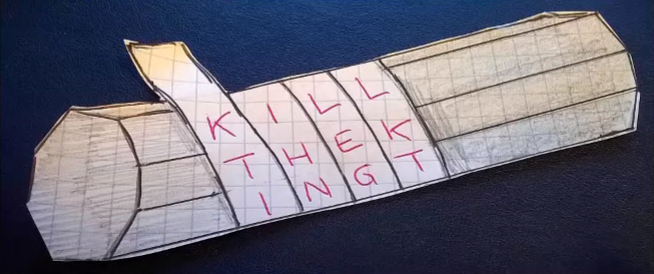
\includegraphics[scale=0.5]{2.png}
\end{center}
\paragraph{Enea Tattico} Un libro qualsiasi con un insieme di lettere segnate, o sostituire le vocali con simboli grafici.
\paragraph{Cifrario di Cesare} Il più antico cifrario di concezione moderna. L'idea di base è che il crittogramma è ottenuto dal messaggio in chiaro \texttt{m} sostituendo ogni lettera con quella di tre posizioni più avanti nell'alfabeto.\\
Es. A $\rightarrow$ D, Z $\rightarrow$ C. La segretezza dipende interamente dalla conoscenza del metodo, era destinato all'uso ristretto da un piccolo gruppo di persone.
\section{Livello di segretezza}
\paragraph{Classificazione} in base al livello di segretezza
\begin{list}{}{}
	\item Cifrari per \textbf{uso ristretto}\\
	Le tecniche con cui si calcola e decifra il crittogramma sono tenute segrete in ogni loro aspetto. Impiegati per comunicazioni classificate (diplomatiche o militari), non adatti per uso di massa.
	\item Cifrari per \textbf{uso generale}\\
	Ogni codice segreto non può essere mantenuto tale per troppo a lungo. La parte segreta si limita alla chiave, nota solamente agli utenti che stanno comunicando.\\
	Vengono studiati dalla comunità, coinvolgendo tantissime persone. Solo la chiave deve essere segreta.\\
	\textbf{Il nemico conosce il sistema}.\\
	Quindi C e D sono note, la chiave \textbf{segreta} \texttt{k} è usata come input sia in C che in D:\\
	\texttt{c = C(m, k)}, \texttt{m = D(c, k)}\\
	Se non si conosce \texttt{k}, anche conoscendo C e D non si possono estrarre informazioni dal crittogramma.\\
	Tenere segreta una sola chiave è più facile che segretare l'intero metodo. Tutti possono usare C e D pubbliche con chiavi diverse, e se un crittoanalista entra in possesso di una chiave posso generarne semplicemente una nuova.
\end{list}
\subsection{Chiavi segreta} Se la segretezza dipende unicamente dalla chiave bisogna proteggersi dagli attacchi a forza bruta, quindi avere un gran numero di chiavi, così da essere immuni da chi le prova tutte.\\
Inoltre la chiave deve essere scelta in modo casuale e non prevedibile, sennò il crittoanalista può provare le chiavi ovvie.
\paragraph{Attacco esauriente} Il crittoanalisa potrebbe sferrare un attacco a forza bruta verificando la significatività delle sequenze \texttt{D(c, k)} $\forall$ \texttt{k}.\\
Se $|$Key$|$ = $10^{20}$ e con un calcolatore che impiega $10^{-6}$ per calcolare \texttt{D(c, k)} servirebbe in media più di un milione di anni per scoprire il messaggi provando tutte le chiavi. Però la segretezza può essere violata con altre tecniche: esistono cifrari più sicuri di altri pur con uno spazio di chiavi più piccoli.\\
Un cifrario complicato non è necessariamente più sicuro e \textbf{mai sottovalutare la bravura del crittoanalista}.
\subsection{Crittoanalista}
\paragraph{Comportamento} Il comportamento di un crittoanalista può essere:
\begin{list}{}{}
	\item \textbf{Passivo}, quando si \textbf{limita ad ascoltare} la comunicazione
	\item \textbf{Attivo}, quando \textbf{agisce sul canale} disturbando la comunicazione o modificando il contenuto dei messaggi.
\end{list}
\paragraph{Attacchi a un sistema crittografico} Hanno l'obiettivo di forzare un sistema. Il metodo e il livello di pericolosità dipendono dalle informazioni in possesso del crittoanalista:
\begin{list}{}{}
	\item \textbf{Cipher Text Attack}: conosce una serie di crittogrammi
	\item \textbf{Known Plain-Text Attack}: conosce una serie di coppie \texttt{(m, c)}
	\item \textbf{Chosen Plain-Text Attack}: si procura coppie \texttt{(m, c)} relative a messaggi in chiaro da lui scelti.\\
	Tutta la crittografia a chiave pubblica è soggetta a questo tipo di attacco (avendo la chiave pubblica, cifro dei messaggi che penso possano passare e ascolto finché non trovo nella comunicazione i crittogrammi in mio possesso).
\end{list}
\paragraph{Man in the Middle} Il crittoanalista si installa sul canale di comunicazione:
\begin{list}{}{}
	\item \textbf{Interrompe le comunicazioni dirette} tra gli utenti Alice e Bob
	\item le \textbf{sostituisce con messaggi propri}
	\item e \textbf{convince} ciascun utente \textbf{che tali messaggi provengano leggitimamente dall'altro} utente.
\end{list}
Quindi il crittoanalista \textbf{Eve si finge Bob agli occhi di Alice e Alice agli occhi di Bob}.
\paragraph{Esiti}
\begin{list}{}{}
	\item Successo pieno, si scopre completamente D o si ottiene la chiave
	\item Successo limitato, si scopre solo qualche informazione ma sufficiente per comprendere il messaggio
\end{list}
\subsection{Situazione attuale}
\paragraph{Cifrari perfetti} Inattaccabili, esistono ma richiedono operazioni complesse, \textbf{chiavi lunghe tanto quanto il messaggio e mai riutilizzabili}.\\
\textbf{Shannon}, 1945 (pubblicato nel 1949 per motivi di segretezza militare): \texttt{m} e \texttt{c} appaiono totalmente scorrelati, come se \texttt{c} fosse una stringa casuale di bit.\\Nessuna informazione può filtrare dal crittogramma. Vedremo la teoria matematica.
\subparagraph{One-Time Pad} Anche detto blocco monouso, sicuro ma per essere usato bene richiede chiavi segrete totalmente casuali e lunghe quanto il messaggio. Come generarla e come scambiarla?
\paragraph{Cifrari attuali} Nella crittografia di massa non si usano cifrari perfetti, ma \textbf{cifrari \textit{dichiarati} sicuri}, inviolati dagli esperti e che usano algoritmi solo esponenziali per decrittare senza chiave. Il tempo per violare un cifrario è enorme e rende l'operazione insostenibile $\rightarrow$ impossibilità \textit{pratica} di forzare il cifrario.
\subparagraph{Dichiarati sicuri} Non è noto se questi problemi matematici richiedano algoritmi \textit{necessariamente} esponenziali o se sono dovuti all'incapacità nostra di trovare metodi più efficienti. Si riconduce a $P = NP$
\subsection{Cifrari odierni}
\paragraph{Advanced Encryption Standard} AES, simmetrico a blocchi con chiavi di 128-256bit, pubblicamente noto e realizzabile su computer di ogni tipo. Il messaggio è diviso a blocchi lunghi quanto la chiave.
\paragraph{Le chiavi} Sono stabilite dai mezzi elettronici (PC, smartphone, terminale...) e su Internet si scambia una chiave per ogni sessione.
\subparagraph{Scambio delle chiavi} La chiave va comunicata in sicurezza su un canale non ancora sicuro. Un'intercettazione nello scambio della chiave compromette il sistema.\\
Nel 1976 viene proposto un algoritmo per generare e scambiare una chiave segreta su un canale insicuro, senza necessità di scambiare informazioni o di incontrarsi in precedenza.\\
Si chiama \textbf{protocollo DH}, ancora largamente utilizzato nei protocolli crittografici su Internet.\\
Si scambiano pezzi di chiave tramite la rete e unendole a informazioni locali si costruisce la chiave.
\subparagraph{Chiave pubblica} Diffie ed Hellman hanno anche proposto la crittografia a chiave pubblica.
\begin{list}{}{}
	\item \textbf{Cifrari simmetrici}: stessa chiave per cifrare e decifrare, nota solo ai due utenti che comunicano. La scelgono di comune accordo e la tengono segreta.
	\item \textbf{Cifrari asimmetrici}: chiavi pubbliche usate per cifrare e chiavi private per decifrare.\\
	\texttt{c = C(m, k$_{pub}$)}\\
	\texttt{m = D(m, k$_{prv}$)}\\
	Si rende necessario che la C sia una one-way trapdoor: calcolare il crittogramma deve essere facile (polinomiale), ma decifrare \texttt{c} deve essere computazionalmente difficile (a meno di conoscere la trapdoor, la chiave privata).
\end{list}
\paragraph{RSA} Rivest, Shamir, Adleman, 1977. Propongono un sistema a chiave pubblico facile da calcolare e difficile da invertire.
\paragraph{Vantaggi}
\begin{list}{}{}
	\item Comunicazione molti a uno\\
	Tutti possono inviare in modo sicuro allo stesso destinatario usando la sua chiave pubblica, ma solo lui può decifrarli. Un crittoanalista non può decifrare anche se conosce C, D e k$_{pub}$
	\item Se $n$ utenti vogliono comunicare servono solo $2n$ chiavi invece delle $n(n-1)/2$ necessarie nei cifrari simmetrici (una coppia per ogni coppia di utenti)
	\item Non è richiesto nessun scambio
\end{list}
\paragraph{Svantaggi}
\begin{list}{}{}
	\item Sono molto lenti rispetto ai cifrari simmetrici (polinomi di terzo grado)
	\item Sono esposti ad attacchi di tipo chosen plain-text, perché conosco la chiave pubblica\\
	Scelgo un numero qualsiasi di messaggi in chiaro, costruisce i crittogrammi relativi e ascolta sul canale confrontando i crittogrammi in transito e se trova un riscontro sa esattamente qual è il messaggio passato.
\end{list}
\paragraph{Come si usa} Oggi si usa un cifrario a chiave segreta (AES) per le comunicazioni di massa, e un cifrario a chiave pubblica per scambiare le chiavi segrete relative al primo senza incontri fisici tra gli utenti.\\
Diventa lento solo lo scambio delle chiavi. Siamo anche al sicuro da attacchi chosen plain-text perché se la chiave è scelta bene risulta imprevedibile dal crittoanalista.
\section{Rappresentazione matematica di oggetti}
Per rappresentare gli oggetti scegliamo dei \textbf{caratteri} da un \textbf{insieme finito} detto \textbf{alfabeto}.\\
Un \textbf{oggetto} è \textbf{rappresentato da una sequenza ordinata di caratteri dell'alfabeto}. L'ordine dei caratteri è importante: a \textbf{oggetti diversi corrispondono sequenze diverse} e \textbf{il numero di oggetti che si possono rappresentare non ha limiti}. Significa che fissando un numero $n$ arbitrariamente grande possiamo sempre creare un numero di oggetti $> n$, con sequenze via via più grande.
\paragraph{Alfabeto} $\Gamma$ con $|\Gamma| = s$ e $N$ oggetti da rappresentare.\\
$d(s, N)$: lunghezza della sequenza più lunga che rappresenta un oggetto dell'insieme. A noi interessa la rappresentazione che minimizza $d(s, N)$, cioè $d_{min}(s, N)$\\
Una rappresentazione è tanto più efficiente quanto $d(s, N)$ si avvicina a $d_{min}(s, N)$
\paragraph{Esempio} $s = 1, \Gamma = \{0\}$ l'unica possibilità è variare la lunghezza $\Rightarrow d_{min}(1, N) = N$, estremamente sfavorevole.\\
$s = 2, \Gamma = \{0, 1\}$, $\forall\:k\geq 1$ ho $2^k$ sequenze di lunghezza $k$. Il numero totale di sequenze lunghe da $1$ a $k$ è $2^{k+1} - 2$ (si esclude anche la sequenza nulla). Con $N$ oggetti da rappresentare $\Rightarrow k \geq \log_2(N+2) - 1 \Rightarrow N$ sequenze diverse tutte di $\log_2(N)$ caratteri.
\paragraph{Efficiente} Codifica efficiente quando c'è questa riduzione logaritmica, \textbf{efficiente} quando \textbf{}. Sequenze della stessa lunghezza è vantaggioso perché non servono caratteri separatori. Per questo è necessario che l'alfabeto contenga almeno due caratteri.\\
La \textbf{notazione posizionale} è una rappresentazione efficiente indipendentemente dalla base $s \geq 2$ scelta. Un intero $N$ è rappresentato con un numero $d$ di cifre $|\: \log_s(N) \leq d \leq \log_s(N) + 1$
\section{Richiamo della teoria della calcolabilità}
\paragraph{Problemi computazionali} Formulati matematicamente di cui cerchiamo una soluzione algoritmica: \textbf{decidibili} (e \textbf{trattabili} o \textbf{non trattabili}), o \textbf{non decidibili}.\\
Calcolabilità $\rightarrow$ \textbf{Algoritmo} e \textbf{problema non decidibile}\\
Complessità $\rightarrow$ \textbf{Algoritmo efficiente} e \textbf{problema intrattabile}.
\paragraph{Numerabilità} Due insiemi $A$ e $B$ hanno lo stesso numero di elementi $\Leftrightarrow$ si può stabilire una \textbf{corrispondenza biunivoca} tra i loro elementi.\\
Questo porta alla definizione di \textbf{numerabile}: un insieme è numerabile $\Leftrightarrow$ i suoi elementi possono essere messi in \textbf{corrispondenza biunivoca con i numeri naturali}.\\
Numerabile significa che \textbf{possiede un'infinità numerabile di elementi}. Esempi: l'insieme dei numeri naturali $N$, l'insieme degli interi $Z$ (avendo $n$ in corrispondenza biunivoca con $2n + 1$ per $n\geq 0$ e $n \leftrightarrow 2|n|$ per $n < 0$, dando la sequenza $0, -1, 1, -2, 2\ldots$) o anche l'insieme dei naturali pari ($2n \leftrightarrow n$)
\paragraph{Enumerazione delle sequenze} Si vuole elencare in uno ordine ragionevole le sequenze di lunghezza finita costruite su un alfabeto finito. Le sequenze non sono in numero finito, quindi non si potrà completare l'elenco.\\
Lo scopo è \textbf{raggiungere qualsiasi sequenza $\sigma$ arbitrariamente scelta in un numero finito di passi}. $\sigma$ deve dunque trovarsi a \textbf{distanza finita} dall'inizio dell'elenco. Non va bene l'ordine del dizionario perché non saprei la posizione della prima stringa che inizia con $b$ perché le stringhe composte da tutte $a$ sono infinite.\\
Si stabilisce un ordine tra i caratteri. Si ordinano prima in lunghezza crescente e, a pari lunghezza, in ordine alfabetico.
\paragraph{Esempio} $\Gamma = \{a, b, \ldots, z\}$, avrei\\
$a, b, \ldots, z,$\\
$aa, ab, \ldots, az, ba, bb, \ldots, bz, \ldots, zz,$\ldots\\
Ad una sequenza arbitraria corrisponde un numero intero, e la sequenza $s$ arbitraria si troverà tra quelle di lunghezza $|s|$ in posizione alfabetica. Quindi ad una sequenza arbitraria $\leftrightarrow$ $n$ che indica la posizione nell'elenco, e ad un numero naturale $n \leftrightarrow$ la sequenza che occupa l'$n$-esima posizione nell'elenco.\\\\
La \textbf{numerazione delle sequenze è fattibile perché sono di lunghezza finita}, anche se illimitata. Cioè per qualunque intero $d$ scelto a priori, esistono sequenze di lunghezza maggiore di $d$. Per sequenze di lunghezza infinita la numerazione non è possibile
\paragraph{Insiemi non numerabili} Insiemi non equivalenti a $N$ come $R$, $(0, 1)$, l'insieme di tutte le linee del piano, insieme delle funzioni in una o più variabili\ldots $\Rightarrow$ l'\textbf{insieme dei problemi computazionali non è numerabile}. Perché un problema computazionale è sempre visualizzabile come una funziona matematica, che associa ad ogni insieme di dati espressi da $k$ numeri interi il corrispondente risultato espresso da $j$ numeri interi $$f:N^k \rightarrow N^j$$
Quindi l'insieme di queste $f$ \textbf{non è numerabile}.
\paragraph{Diagonalizzazione}
$F = \{$ funzioni $f\:|\: f: N \rightarrow \{0, 1\}\}$, ogni $f\in F$ è rappresentata da una sequenza infinita
\begin{list}{}{}
	\item $x$ 0 1 2 3 \ldots n \ldots
	\item $f(x)$ 0 1 0 1 \ldots 0 \ldots
\end{list}
ma se è possibile è rappresentabile con una regola (f 0 se x pari 1 se x dispari)\\
Per assurdo, ipotizzo F numerabile. Si può assegnare ad ogni funzione un numero progressivo nella numerazione e costruire una tabella infinita con tutte le funzioni.
\begin{center}
	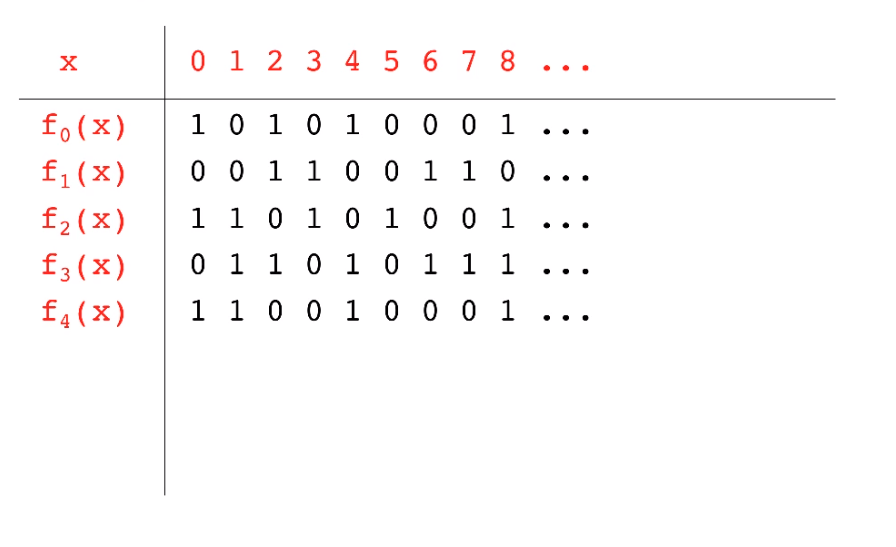
\includegraphics[scale=0.6]{3.png}
\end{center}
Definisco $g(x)$ = $\left\{ \begin{array}{l l}
0 & f_x(x) = 1\\ 1 & f_x(x) = 0
\end{array} \right. \Rightarrow g$ non può corrispondere a nessuna delle $f_i$ della tabella, perché differisce da tutte le funzioni almeno nella diagonale principale.\\
$g(x)\:\:|\:\:\:0\:1\:1\:1\ldots$\\
Per assurdo $\exists\:j\:|\:g(x) = f_j(x) \Rightarrow g(j) = f_j(j)$ ma per la definizione $g(j)$ è il complemento di $f_j(j)$, quindi $g(j) \neq f_j(j)$ \textbf{contraddizione}.\\
Per qualunque numerazione scelta esiste sempre almeno una funzione esclusa, quindi $F$ non è numerabile.
\subsection{Algoritmi}
\paragraph{Algoritmi} la \textbf{formulazione di un algoritmo}, una sequenza finita di operazioni, completamente e univocamente determinate, \textbf{dipende dal modello di calcolo utilizzato}.\\
Qualunque modello si scelga, gli algoritmi devono essere descritti da sequenze finite di caratteri di un alfabeto finito $\Rightarrow$ sono \textbf{possibilmente infiniti ma numerabili}.
\paragraph{Problemi computazionali} Sono \textbf{funzioni matematiche} che associano ad ogni insieme di dati il corrispondente risultato, e \textbf{non sono numerabili} come visto prima.
\paragraph{Problema della rappresentazione} C'è una drastica perdita di potenza, perché gli algoritmi sono numerabili ma sono meno dei problemi computazionali $$|\{Problemi\}| >> |\{Algoritmi\}|$$
$\Rightarrow$ \textbf{esistono problemi privi di un corrispondente algoritmo di calcolo}. Per esempio, il problema dell'arresto.
\paragraph{Lezione di Turing} \textit{Non esistono algoritmi che decidono il comportamento di altri algoritmi esaminandoli dall'esterno, cioè senza passare dalla loro simulazione}.
\subsection{Modelli di calcolo}\begin{center}
La teoria della calcolabilità dipende dal modello di calcolo?\\
Oppure\\
la decidibilità è una proprietà del problema?
\end{center}
\pagebreak
I linguaggi di programmazione esistenti sono tutti equivalenti?\\
Ce ne sono di alcuni più potenti/più semplici di altri?\\
Ci sono algoritmi descrivibili in un linguaggio ma non in un altro?\\
È possibile che problemi oggi irrisolvibili possano essere risolti in futuro con altri linguaggi o altri calcolatori?\\
Le teorie della calcolabilità e della complessità dipendono dal modello di calcolo?
\paragraph{Tesi di Church-Turing} Tutti i \textit{ragionevoli} modelli di calcolo \textbf{risolvono esattamente la stessa classe di problemi}, quindi \textbf{si equivalgono nella possibilità di risolvere i problemi} pur operando con diversa efficienza.
\begin{center}
\textbf{Tesi C-H: la decidibilità è una proprietà del problema}
\end{center}
Incrementi qualitativi sui calcolatori o sui linguaggi di programmazione servono \textbf{solo} ad abbassare i tempi di esecuzione o rendere più agevole la programmazione.
\subsection{Decidibilità e trattabilità}
Ci sono quindi problemi che non possono essere risolti da nessun calcolatore, indipendentemente dal tempo impiegato (\textbf{problemi indecidibili}).\\
Ci sono poi problemi decidibili che possono richiedere tempi di risoluzione esponenziali nella dimensione dell'istanza (\textbf{problemi intrattabili}).\\
Ci sono poi problemi che possono essere risolti con algoritmi di costo polinomiale nella dimensione dell'inpu\\(\textbf{problemi trattabili}).\\
Abbiamo poi una famiglia di problemi il cui stato non è noto: clique (cricca), cammino hamiltoniano\ldots Sappiamo risolverli (decidibili) con algoritmi di costo esponenziale, ma non abbiamo limiti inferiori esponenziali. I migliori limiti inferiori sono polinomiali: c'è un gap fra il limite inferiore (polinomiale) e costo della migliore soluzione a disposizione (esponenziale) (\textbf{presumibilmente intrattabili}).
\subsubsection{Notazione}
Studiamo la dimensione dei dati trattabili in funzione dell'incremento della velocità del calcolatori.\\
Dati i calcolatori $C_1$, $C_2$ ($k$ volte più veloce di $C_1$) e tempo di calcolo a disposizione $t$, avrò $n_1$ dati trattabili in tempo $t$ su $C_1$ e $n_2$ trattabili in tempo $t$ su $C_2$.\\\\
Si \textbf{osserva} che \textbf{usare $C_2$ per un tempo $t$ equivale a usare $C_1$ per un tempo $k\cdot t$}.
\paragraph{Algoritmi polinomiali} Un algoritmo polinomiale che risolve il problema in $c\cdot n^s$ secondi, con $c$ ed $s$ costanti.
\begin{list}{}{}
	\item[$C_1$] $c\cdot n_1^s = t \Rightarrow n_1 = (t/c)^{1/s}$
	\item[$C_2$] $c\cdot n_2^s = t \Rightarrow n_2 = k^{1/s}\cdot(t/c)^{1/s}$
	\item[$\Rightarrow$] $n_2 = k^{1/s}\cdot n_1$, miglioramento di un fattore \textbf{moltiplicativo} $k^{1/s}$
\end{list}
\paragraph{Algoritmi esponenziali} Un algoritmo polinomiale che risolve il problema in $c\cdot 2^n$ secondi, con $c$ costante.
\begin{list}{}{}
	\item[$C_1$] $c2^{n_1} = t \Rightarrow 2^{n_1} = t/c$
	\item[$C_2$] $c2^{n_2} = k\cdot t \Rightarrow 2^{n_1} = k\cdot t/c = k2^{n_1}$
	\item[$\Rightarrow$] $n_2 = n_1 + \log_2(k)$, miglioramento di un fattore \textbf{additivo} $\log_2(k)$
\end{list}
Di conseguenza \textbf{un algoritmo efficiente è di gran lunga più importante di un calcolatore più potente}.
\subsection{Tipologie di problemi}
Dato un problema $\Pi$ su un insieme di istanze in ingresso $I$ con un insieme di soluzioni $S$.
\paragraph{Problemi decisionali} Richiedono una risposta binaria $S=\{0, 1\}$, quindi istanze positive $x\in I\:|\:\Pi(x) = 1$ o negative $x\in I\:|\:\Pi(x) = 0$. Esempio: verifica se un numero è primo, o se un grafo è connesso.\\
La teoria della complessità computazionale è definita principalmente in termini di problemi di decisione: risposta binaria, quindi il tempo per restituire la risposta è costante, e la complessità di un problema è già presente nella versione decisionale.
\paragraph{Problemi di ricerca} Data un'istanza $x$, richiede di restituire una soluzione $s$.
\paragraph{Problemi di ottimizzazione} Data un'istanza $x$, si vuole trovare la \textbf{migliore} soluzione $s$ tra tutte quelle possibili. Esempio: clique di dimensione massima, cammino minimo\ldots
\subsection{Classi di complessità}
Dato un problema \textbf{decisionale} $\Pi$ ed un algoritmo $A$, diciamo che \textbf{$A$ risolve $\Pi$} se, data un'istanza di input $x$, $A(x) = 1 \Leftrightarrow \Pi(x) = 1$\\
$A$ risolve $\Pi$ in \textbf{tempo $t(n)$ e spazio $s(n)$}.
\paragraph{Classi Time e Space}
\begin{list}{}{}
	\item Time($f(n)$): insieme dei \textbf{problemi decisionali che possono essere risolti in tempo O($f(n)$)}
	\item Space($f(n)$): insieme dei \textbf{problemi decisionali che possono essere risolti in spazio O($f(n)$)}
\end{list}
\paragraph{Classe P} Classe dei problemi risolvibili in \textbf{tempo} polinomiale nella dimensione dell'istanza di input.\\
\textbf{Algoritmo polinomiale} nel tempo: $\exists\:c, n_0 > 0\:\:|\:\:$ il numero di passi elementari è al più $n^c$ per ogni input di dimensione $n > n_0$.
\paragraph{Classe PSPACE} Classe dei problemi risolvibili in \textbf{spazio} polinomiale nella dimensione dell'istanza di input. Molto più grande di P.\\
\textbf{Algoritmo polinomiale} nello spazio: $\exists\:c, n_0 > 0\:\:|\:\:$ il numero di celle di memoria è al più $n^c$ per ogni input di dimensione $n > n_0$.
\paragraph{Classe EXPTIME} Classe dei problemi risolvibili in tempo esponenziale nella dimensione dell'istanza di input.
$$P\subseteq PSPACE \subseteq EXPTIME$$
Non è noto se queste inclusioni siano note, ad oggi. L'unico risultato dimostrato finora riguarda P ed EXPTIME: esiste un problema che può essere risolto in tempo esponenziale ma per cui il tempo polinomiale non è sufficiente (es: torri di Hanoi).
\subsection{Certificato}
Per alcuni problemi, per le istanze accettabili (istanze in cui la risposta del problema decisionale è si), è possibile certificare che quell'istanza è accettabile con un certificato $y$ che può convincerci dell'accettabilità.\\
Per clique, il certificato è il sottoinsieme di $k$ vertici che forma la clique. Per il cammino hamiltoniano è la permutazione degli $n$ vertici che formano il cammino. Per SAT, sono le assegnazioni che rendono vera la formula. Il certificato ha dimensione polinomiale ($k, n$) e la verifica del certificato è lineare.\\
Una volta che ho il certificato lo vado a verificare: attestato breve di esistenza di una soluzione con determinate proprietà. Si definisce solo per istanze accettabili, perché spesso la non accettabilità non è facile costruire un certificato.
\paragraph{Idea} Usare il costo della verifica di un certificato per un'istanza accettabile per \textbf{caratterizzare la complessità del problema} stesso.\\
Un problema è \textbf{verificabile in tempo polinomiale} se: tutte le istanze accettabili ammettono un certificato di lunghezza polinomiale ed esiste un algoritmo di verifica polinomiale in n.
\paragraph{Classe NP} Classe dei problemi decisionali \textbf{verificabili in tempo polinomiale}. (NP = polinomiale su macchine non deterministiche)
\paragraph{P $\subset$ NP?} Ovviamente si, ogni problema in P ammette un certificato verificabile in tempo polinomiale: eseguo l'algoritmo che risolve il problema per costruire il certificato.\\
Quello che non sappiamo è $P = NP$ oppure $P \neq NP$. Si pensa $P \neq NP$.\\
Si possono individuare i problemi più difficili in NP, ovvero quelli candidati ad appartenere ad NP se $P \neq NP$: sono i problemi NP-completi, quelli per cui se esiste un algoritmo polinomiale per risolvere un NP-completo allora tutti i problemi NP potrebbero essere risolti in tempo polinomiale e quindi P = NP.\\
Quindi tutti i problemi NP-completi sono risolvibili in tempo polinomiale oppure nessuno lo è.\\\\
Tutti i problemi NP-completi possono essere ridotti l'un l'altro, sono NP-equivalenti.
\paragraph{Gerarchia delle classi secondo le attuali congetture}
\begin{center}
	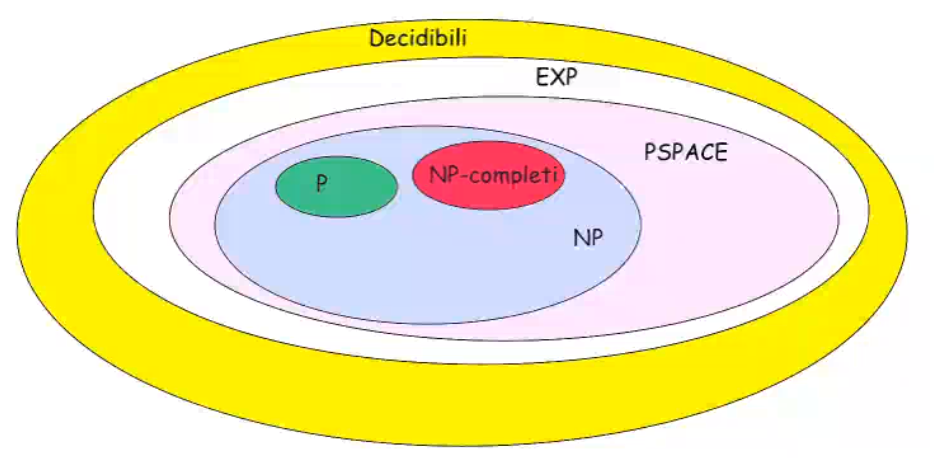
\includegraphics[scale=0.75]{4.png}
\end{center}
La fattorizzazione ad esempio $\in NP - (P \cup NPcompleti)$, infatti è risolto in tempo polinomiale su macchine quantistiche.
\subsection{Classi co-P e co-NP}
C'è molta differenza tra certificare l'esistenza e certificare la non esistenza di una soluzione. Dato un problema $\Pi$ possiamo definire co$\Pi$ che accetta tutte e sole le istanze rifiutate da $\Pi$.\\
La classe coP è la classe per cui co$\Pi\in$ P. P = coP, i problemi complementari e i co-complementari (originali) si possono entrambi risolvere in tempo polinomiale: risolvo il problema complementare e complemento il risultato.\\\\
Questo non vale per coNP, la classe per cui co$\Pi\in$ NP. Si congettura che siano diverse, se la congettura è vera allora $P\neq NP$
\begin{center}
	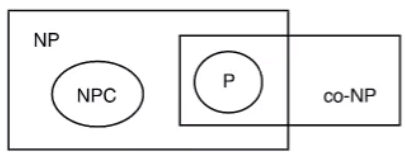
\includegraphics[scale=0.5]{5.png}
\end{center}
\chapter{Sequenze Casuali}
\section{Esempi di algoritmi numerici}
\paragraph{Algoritmo di Euclide} Algoritmo per il calcolo dell'MCD fra due interi.\\
Suppongo due interi $a$, $b$ con $a \geq b$, $a > 0$ e  $b \geq 0$\\
MCD$(a,b) = \left\{ \begin{array}{l l}
a & b = 0\\
MCD(a, a\: mod\: b) & else
\end{array}\right.$
\subparagraph{Valutazione complessità} Data I istanza di input composta da $a$, $b$, vengono rappresentati ad esempio in base due. Quindi la dimensione $n$ dell'istanza di input I $n = \:|I|\:=\Theta(\log a + \log b) = \Theta(\log a)$.\\
L'algoritmo è ricorsivo, quindi bisogna valutare il numero delle chiamate ricorsive, che dipenderanno dai dati. Ci saranno istanze in cui si termina subito (ad esempio se $a$ multiplo di $b$, cioè $a$ mod $b = 0$). In generale, \textbf{il numero di chiamate cresce con $\log a$}, perché $a$ mod $b$ rimpiazza $a$.\\\\
Si osserva che $a$ mod $b < \frac{a}{2}$\\
Questo perché $a = qb + (a$ mod $b)$ e siccome per ipotesi $a \geq b \Rightarrow b \geq 1$ e lo è anche $q \Rightarrow a \geq b + (a$ mod $b) > (a$ mod $b) + (a$ mod $b)$ perché $b > (a$ mod $b)$.\\ $\Rightarrow 2(a$ mod $b) < a \Rightarrow (a$ mod $b) < \frac{a}{2}$.\\
Prima chiamata su $a, b$.\\
Seconda su $b, (a$ mod $b)$.\\
Terza su $(a$ mod $b), (b$ mod $(a$ mod $b))$.\\
Quindi ad ogni chiamata a si riduce almeno della metà, e lo possiamo fare al massimo $\log a$ volte\\
\textbf{Quindi avrò $O(\log a)$ ricorsioni}.\\\\
Il costo del calcolo del modulo è $O(\log a \cdot \log b) = O(\log^2 a)$\\
Complessivamente T($n$) = $O(\log^3 a) = O(n^3)$ \textbf{polinomiale nella dimensione dell'istanza $|I|$} (cioè nel numero di cifre), \textbf{polilogaritmico nel valore dei dati}
\paragraph{Test di primalità} Versione inefficiente.\\
Primo(N): \texttt{for} ($i$ = 2, $i\leq \sqrt{N}$, $i++$)\\
\texttt{if} $N\% i == 0$ \texttt{return false}\\
\texttt{else} \textit{a fine ciclo} \texttt{return true}.\\
Uso la proprietà che se $N$ non è primo allora ha almeno un divisore $\leq \sqrt{N}$.
\subparagraph{Valutazione di complessità} $I = N, \:|I|\: = \Theta(N) = n$\\
Ho $\sqrt{N}$ iterazioni, ciascuna di costo $\Theta(\log^2 N)$\\\\
$T(n) = O(\sqrt{N} \cdot \log^2 N) = O(2^{\frac{n}{2}}\cdot n^2)$ \textbf{pseudopolinomiale}, cioè \textbf{polinomiale nel valore di N ma esponenziale nella dimensione $|I|\: = n$}.
\pagebreak
\section{Casualità}
\paragraph{Problema} Data una sequenza binaria, vogliamo \textbf{capire se è una sequenza casuale} o meno. Le sequenze casuali sono importanti sia per la generazioni delle classi, sia perché \textbf{in crittografia spesso si ricorrono ad algoritmi randomizzati che usano sequenze casuali per funzionare}.
\paragraph{Significato algoritmico della casualità} Vedendo la teoria di Kolmogorov. Prendiamo due sequenze
\begin{list}{}{}
	\item $h$: 1111\ldots 1 lunga $n$
	\item $h'$: 10110110101011010100101\ldots 0
\end{list}
\textbf{La prima è molto facile da descrivere} (\textit{scrivi $n$ "uni"}), mentre \textbf{descrivere la seconda è molto meno pratico}: l'intuizione è che \textbf{una sequenza casuale non si può descrivere in modo compatto}.\\
Ponendo $n$ = 20, la probabilità di generare $h$ è $P(h = (1/20)^{20}$, $P(h') = (1/20)^{20}$ (1/2 per generare 1, 1/2 per generare 0\ldots).\\
$A_h$ algoritmo che genera $h$. Formalizzabile semplicemente (\textit{genera $n$ uni})\\
$|A_h|$ = $\#$ bit di $A_h$ codificato in binario $= \log n +$ const (la parte costante è la generazione e l'output, varia solo $n$) $\Rightarrow$ con $\log n$ bit ne abbiamo descritti $n$.\\
$A_{h'} =$ \texttt{print} $h'$, $|A_{h'}| > |n| = |h'|$\\\\
L'intuizione è \textbf{una sequenza binaria è casuale se non ammette un algoritmo di generazione la cui rappresentazione binaria sia più corta di $h$}. Se posso usare meno bit vuol dire che la sequenza ha una qualche regolarità.
\paragraph{Sistemi di calcolo} Sono un infinità numerabile $S_1\ldots S_i\ldots$\\
Prendiamo $S_i$, $p$ programma che genera la sequenza $h$ nel sistema $S_i$, cioè $S_i(p) = h$\\
\textbf{Def}: \textbf{la complessità di Kolmogorov di $h$ nel sistema $S_i$ è $K_{S_i}(h) = min\{\:|p|\: \:|\: S_i(p) = h\}$} cioè la minima lunghezza del programma $p$ che in $S_i$ genera $h$ stessa.\\\\
Se la sequenza $h$ non segue alcuna legge semplice di regolarità, allora \textbf{il più breve programma in grado di generarla dovrà contenerla al suo interno}, cioè sarà almeno lungo quanto la sequenza stessa e la genererà trasferendola in output. Quindi $K_{S_i}(h) = \:|h|\: +$ \texttt{const}$_i$. La costante è la parte di programma che trasferisce in output, dipende da $S_i$ ma non ha $h$.
\paragraph{Sistema di calcolo universale} Tra tutti i sistemi di calcolo possibili ne esiste uno \textbf{universale in grado di simulare tutti gli altri}. Lo chiamiamo $S_u$ e lo prendiamo in considerazione.\\
Supponiamo $p\:|\:S_i(p) = h$, allora $S_u(\langle i, p\rangle) = S_i(p) = h$. Ottengo $q = \langle i, p\rangle$ programma che genera $h$ in $S_u$\\\\
$|q| = |\langle i,p\rangle| = |i| + |p| = \log_2 i + |p|$ quindi la lunghezza di $q$ dipende da $i$ ma non da $h$.\\
$\forall\:h\:\:\forall\: i\:\:K_{S_u}(h) \leq K_{S_i}(h) + C_i$\\
L'uguale vale per le sequenze generate per simulazione di $S_i$ non essendoci per $S_u$ algoritmi più "brevi".\\Il minore vale per sequenze generabili con programmi più corti (ad esempio per simulazione su un altro sistema $S_j\neq S_i$).
\paragraph{Def} La complessita di Kolmogorov di una sequenza $h$ è $K(h) = K_{S_u}(h)$
\subsection{Sequenze casuali}
\paragraph{Sequenza casuale} Una sequenza $h$ è casuale se $K(h) \geq |h| - \lceil\log_2 h\rceil$\\
Non entra in gioco come genero la sequenza, la \textbf{casualità è una proprietà della sequenza}.
\paragraph{Conteggio delle sequenze} $\forall\: n, \exists$ sequenze casuali (secondo Kolmogorov) di lunghezza $n$\\
\textbf{Dim}: $n$, $S = 2^n$ \# sequenze binarie di lunghezza $n$\\
T = \# sequenze di lunghezza $n$ NON casuali. L'obiettivo è dimostrare che T $<$ S.\\
Pongo $N$ = \# sequenze binarie di lunghezza $< n - \lceil \log_2 n\rceil = \sum_{i=0}^{n-\lceil \log n\rceil - 1} 2^i = s^{n-\lceil \log n\rceil} - 1$\\
Tra queste $N$ sequenze ci sono anche i programmi che generano le T sequenze non casuali di lunghezza $n$.\\
$\Rightarrow T\leq N < S \Rightarrow T < S$\\
Quindi non solo esistono ma sono anche la \textbf{maggioranza}, essendo enormemente più numerose di quelle non casuali. Lo vediamo studiando il rapporto $$\frac{T}{S}\leq \frac{N}{S} = \frac{2^{n - \lceil\log n\rceil}}{2^n} - \frac{1}{2^n} < \frac{1}{2^{\lceil\log n\rceil}}\:\:\:\lim_{n\to +\infty} \frac{T}{S} = 0$$
\paragraph{Stabilire la casualità} Data una sequenza arbitraria di lunghezza $n$, stabilire se è casuale secondo Kolmogorov è un problema \textbf{indecidibile}.\\
\textbf{Dim}: per assurdo suppongo esista un algoritmo Random $|$ Random($h$) = $\left\{\begin{array}{l l}
1 & h\:casuale\\
0 & altrimenti
\end{array}\right.$ \\
Possiamo costruire l'algoritmo Paradosso che enumera tutte le possibili sequenze binarie in ordine crescente di lunghezza.\\\\
Paradosso:\\\texttt{for} (binary h = 1 $\to$ infty) \texttt{do}\\
\texttt{if} $(|h| - \lceil\log |h|\rceil > |P|\:\&\&$ Random($h$) == 1) \texttt{return} $h$\\\\
$P$ è una sequenza binaria che rappresenta la codifica del programma complessivo Paradosso + Random, quindi $|P| = |$Paradosso$| + |$Random$|$, costante che non dipende da $h$, perché la sequenza $h$ non compare in $P$ ma solo come nome di variabile. Il valore rimane registrato fuori dal programma.\\
\textbf{Paradosso quindi restituisce come risultato la prima sequenza casuale} $|\:|h| - \lceil\log_2 |h|\rceil > |P|$\\
Quindi se $\exists$ sequenze casuali di qualsiasi lunghezza, quindi certamente ne esisterà una che soddisfa entrambe le condizioni dell'\texttt{if}, che viene generata.\\
Ma la prima condizione mi dice che il programma rappresentato da $P$ è breve e genera $h$, quindi $h$ non è casuale perché prodotta con un programma breve.\\
Quindi $K(h) \leq |P|$, cioè $P$ genera $h$) ma $|P| < |h| l \lceil\log_2|h|\rceil$ quindi $h$ non è casuale.\\
Ma la seconda condizione dice $h$ casuale, giungendo ad un \textbf{paradosso} dato dall'assumere l'esistenza di Random.
\subsection{Sorgente binaria casuale}
\paragraph{Generatore} Genera una sequenza di bit con queste proprietà:
\begin{enumerate}
	\item P(0) = P(1) = 1/2, cioè genera 1 o 0 a pari probabilità.\\
	Si può indebolire richiedendo P(0) $>$ 0, P(1) $>$ 0 immutabili nel tempo della generazione.
	\item La generazione di un bit è indipendente dalla generazione degli altri.\\
	$\Rightarrow$ non si può prevedere il valore di un bit osservando quelli già generati.
\end{enumerate}
Perché possiamo indebolire la prima proprietà? Supponiamo di essere in un caso in cui P(0) $>$ P(1), allora è \textbf{sempre possibile bilanciare la sequenza}.\\
Supponiamo di generare 001100111000010100 e si \textbf{dividono a coppie} 00 11 00 11 10 00 01 01 00 e si scartano le coppie uguali. Si associano le coppie miste, ad esempio 01 $\rightarrow$ 0 e 10 $\rightarrow$ 1. Si presentano in modo equiprobabile, quindi la sequenza si ribilancia ottenendo 100 (caso poco significativo perché sequenza corta).
\paragraph{Esistono queste sorgenti?} Non si sa. Nella pratica non è possibile garantire la perfetta casualità o l'indipendenza. Quindi sfrutteremo le casualità presenti in processi fisici o processi software.
\subsubsection{Generatore di sequenze brevi}
\paragraph{Fenomeni casuali presenti in natura} Ad esempio il rumore su un microfono o il tempo di decadimento di alcune particelle, sfruttabili come sorgenti di casualità.\\
Il problema di questo approccio è che bisogna non avere accesso fisico ai dispositivi usati (es: microfono manomesso), oltre alla difficoltà pratica di usare certe sorgenti.
\paragraph{Processi software} Come la temperatura, la posizione della testina del disco fisico\ldots
\paragraph{Pseudocasuale} Si genera la casualità \textbf{mediante un algoritmo}, \textbf{cercandola all'interno di processi matematici}. \textbf{Generatore di numeri pseudo-casuali}: ad esempio \texttt{rand()} del C.\\
Perché pseudocasuali? Perché sono algoritmi deterministici e brevi, quindi non risultano casuali secondo Kolmogorov.
\subparagraph{Come funzionano?} Partono da un \textit{seed} (seme), breve sequenza che viene amplificata per creare una sequenza più lunga. Quindi un generatore è un \textbf{amplificatore di casualità}.
\begin{list}{}{}
	\item Input: seme (sequenza o valore breve)
	\item Output: flusso di bit arbitrariamente lungo e periodico.\\
	Al suo interno contiene una sottosequenza che si \textbf{ripete}, quindi \textbf{un generatore è tanto migliore tanto più è lungo il suo periodo}
	\item Avengo $s$ = \# bit nel seme e $n$ lunghezza della sequenza ottenuta dal generatore, con $n >> s$, ho \textbf{una sequenza diversa per ogni seme}, con $2^s$ possibili semi.
	\\\# sequenze diverse $2^s << 2^n$ \# sequenze possibili
\end{list}
\paragraph{Generatore lineare} $x_i = (a\cdot x_{i-1} + b)$ mod $n$ con $a,b,n$ interi positivi.\\
Il seme è un valore intero iniziale casuale $x_0$, quindi quando $x_i$ = $x_0$ la sequenza si ripete.\\
Dobbiamo avere MCD$(b,n)=1$, $(a-1)$ divisibile per ogni fattore primo di $n$ e $(a-1)$ dev'essere un multiplo di 4 se anche $n$ lo è.\\
Servono per garantire che il generatore produca una permutazione degli interi da 0 a $m-1$
\section{Test statistici}
Per valutare le sequenze prodotte da un generatore pseudocasuale.\\
Si valuta se la sequenza presenta le proprietà tipiche di una sequenza casuale:
\begin{list}{}{}
	\item \textbf{test di frequenza}
	\item \textbf{poker test}: se sottosequenze siano distribuite in modo equo
	\item \textbf{test di autocorrelazione}: verifica che non ci siano regolarità nella sequenza ottenuta
	\item \textbf{run test}: verifica se sottosequenze massimali di elementi tutti ripetuti abbiano una distribuzione esponenziale negativa, cioè più sono lunghe meno sono frequenti.
\end{list}
Per le applicazioni crittografiche si richiede anche il \textbf{test di prossimo bit}, molto severo che implica tutti gli altri 4 test statistici. Intuitivamente, verifica che sia impossibile prevedere gli elementi della sequenza prima di generarli.
\paragraph{Test di prossimo bit} Un generatore binario \textbf{supera} il test di prossimo bit \textbf{se non esiste un algoritmo polinomiale in grado di prevedere l'$i+1$-esimo bit della sequenza a partire dalla conoscenza degli $i$ bit precedentemente generati con probabilità maggiore di 1/2}.\\
Quindi se si hanno a disposizione risorse polinomiale non si può prevedere il prossimo bit. I generatori che superano questo test sono detti \textbf{generatori crittograficamente sicuri}.
\paragraph{Generatore polinomiale} Non è crittograficamente sicuro.\\
$x_i = (a_1 x_{i-1}^t + a_2 x_{i-1}^{t-1} + \ldots + a_t x_{i-1} + a_{t-1})$ mod $n$\\
$r_i = \frac{x_i}{n}$
\section{Generatori crittograficamente sicuri}
\paragraph{Come costruire generatori crittograficamente sicuri}
Si ricorre alle \textbf{funzioni one-way}: funzioni facili da calcolare ma difficili da invertire, cioè \textbf{computabili in tempo polinomiale ($x\mapsto f(x)$)}, ma \textbf{computazionalmente difficile invertire la funzione ($y\mapsto x=f^{-1}(y)$)}. Come costruire queste funzioni?
\paragraph{Idea} Con $f$ one-way, scelgo il seme $x_0$. Genero $S$: $x$ $f(x)$ $f(x_1)=f(f(x))$ \ldots $x_i = f(f(\ldots(x_{i-1})\ldots))$\\
Cioè si itera l'applicazione della funzione one-way un numero arbitrario di volte. L'\textbf{idea è restituire la sequenza al contrario}, perché se conosco $x_{i+1}$ non riesco a calcolare facilmente $x_i$.\\
Ogni elemento della sequenza S si può calcolare efficientemente con l'elemento precedente, ma non dai valori successivi perché $f$ è one-way. Si calcola S per un certo numero di passi senza svelare il risultato e si comunicano gli elementi in ordine inverso. Ogni elemento non è prevedibile in tempo polinomiale pur conoscendo quelli comunicati.
\paragraph{Generatori binari crittograficamente sicuri} Si usano i \textbf{"predicati \textit{hard core}" delle funzioni one-way}.\\
Un predicato hard core di una funzione one-way $f(x)$ è $b(x)$ se $b(x)$ è facile da calcolare quando $x$ è noto, ma è difficile da prevedere se si conosce $f(x)$.\\\\
Un esempio di funzione one-way è l'elevamento a quadrato in modulo ($f(x) = x^2$ mod $n$ con $n$ non primo). Un predicato hard core è "$b(x) = x$ è dispari"
\paragraph{Generatore BBS} Crittograficamente \textbf{sicuro}.\\
$n = p\cdot q$, con $p$ e $q$ primi \textbf{grandi}.
\begin{list}{}{}
	\item $p$ mod 4 = 3
	\item $q$ mod 4 = 3
	\item $2\lfloor \frac{p}{4}\rfloor + 1$ e $2\lfloor \frac{q}{4}\rfloor + 1$ \textbf{primi fra loro}
	\item[$\Rightarrow$] $y$ coprimo con $n$, si calcola $x_0 = y^2$ mod $n$ e \textbf{si usa come seme} per \textbf{calcolare una successione di $m\leq n$ interi}
	\item $x_i = (x_{i-1})^2$ mod $n$\\
	$b_i = 1 \Leftrightarrow x_{n-i}$ è dispari
	\begin{list}{}{}
		\item $b_1 = 1 \Leftrightarrow x_{n-1}$ dispari
		\item $b_0 = 1 \Leftrightarrow x_{n}$ dispari
	\end{list}
\end{list}
Quindi $x_0 = b_n$, ottengo una sequenza del tipo
\begin{list}{}{}
	\item $x_0 \rightarrow x_1 \rightarrow \ldots \rightarrow x_{n-1} \rightarrow x_n$
	\item[$\Rightarrow$] $b_n \rightarrow b_{n-1} \rightarrow \ldots \rightarrow b_1 \rightarrow b_0$\\
	La \textbf{sequenza viene restituita in ordine inverso} $b_0 b_1\ldots$
\end{list}
\subsection{Generatori di numeri pseudocasuali basati su cifrari simmetrici}
\paragraph{Idea} Prendere un cifrario simmetrico e la sua chiave. Anziché usarlo per costruire un crittogramma, si sostituisce il messaggio da cifrare con un \textbf{seme iniziale} legato al generatore. Si comincia a cifrare in questo modo: produce una sequenza imprevedibile per le proprietà del cifrario.\\
Di seguito, un esempio approvato dal FIPS:
\begin{multicols}{2}
\begin{list}{}{}
	\item Usa il DES
	\item $r$ = \# bit delle parole che vengono prodotte\\($r = 64$ nel DES)
	\item $s$ = seme casuale di $r$ bit
	\item $m$ = \# parole da produrre
	\item $k$ = chiave segreta del cifrario
\end{list}
\columnbreak
\begin{lstlisting}
Generatore(s, m){ //flusso di output di m*r bit
	d = <rapp. su r bit di data e ora>;
	y = C(d, k);
	z = s;
	for (i = 1; i <= n; i++) {
		xi = C(y xor z, k);
		z = C(y xor xi, k);
		output(xi);
	}
}
\end{lstlisting}
\end{multicols}
\section{Algoritmi randomizzati}
Si dividono in due classi fondamentali:
\begin{list}{}{}
	\item Algoritmi \textbf{Las Vegas}\\
	Generano un \textbf{risultato sicuramente corretto} in un \textbf{tempo probabilmente breve}.\\
	Caso tipico: quick sort. Qualche passo a caso per cercare di evitare i casi sfavorevoli.
	\item Algoritmi \textbf{Montecarlo}\\
	Generano un \textbf{risultato probabilmente corretto} in un \textbf{tempo sicuramente breve}.\\
	\textbf{Probabilità di errore} deve essere \textbf{arbitrariamente piccola e matematicamente misurabile}.\\
	Caso tipico: test di primalità.
\end{list}
\subsection{Test di primalità (Miller, Rabin)}
\begin{list}{}{}
	\item $N$ intero (dispari) da testare di $n$ bit\\
	$\Rightarrow$ N-1 è pari, $N-1 = 2^w \cdot z$ con $z$ dispari, $w$ esponente della potenza di 2 più grande che divide $N-1$\\
	Es: $N=21, N-1=20 = 2^2\cdot 5$ quindi $z=5, w=2$
	\item Da $N$, calcolo $N-1\rightarrow\frac{N-1}{2}\rightarrow\frac{N-1}{4}\rightarrow\ldots\rightarrow z = 1$ quindi \# divisioni per 2 $\leq\log N = n$ volte\\
	Quindi trovo $w$ e $z$ in maniera efficiente, $O(n)$ passi
	\item Sia quindi $N$ primo e $2\leq y \leq N-1$ arbitrario detto \textit{testimone}, allora
	\begin{list}{}{}
		\item[P1] MCD(N,$y$) = 1, per la primalità
		\item[P2] ($y^z$ mod $N = 1$) $\vee$ ($\exists\:i\:\:0\leq i \leq w-1\:|\:y^{2^i \cdot z}$ mod $N = -1$)
	\end{list}
	Se una delle due proposizione è falsa allora N non è primo, ma ci sono numeri composti che verificano P1 e P2 ma non sono primi (sono pochi).
\end{list}
\subparagraph{Lemma 1} (Miller, Rabin) $N$ è composto, allora il numero di testimoni $y$ che soddisfano i predicati è basso.\\
Cioè $N$ composto $\Rightarrow$ il numero di interi $y\:|\:2\leq y \leq N-1$ che soddisfano entrambi i predicati P1 e P2 è minore di $N/4$\\
La probabilità di scegliere un testimone che rende veri P1 e P2 $< \frac{N/4}{N-2} < \frac{1}{4}$
\subparagraph{N} $y$ scelto a caso in $[2, N-1]$:
\begin{list}{}{}
	\item se uno dei due predicati è \textbf{falso} $\rightarrow N$ è \textbf{certamente composto}
	\item se sono entrambi veri $\Rightarrow N$ è composto con probabilità $< \frac{1}{4}$, dunque $N$ è primo con probabilità $> \frac{3}{4}$
\end{list}
Iterando il test $k$ volte, la probabilità di errore diventa $< \left(\frac{1}{4}\right)^k$, con $k=30$ diventa inferiore al $10^{-18}$.\\
Di seguito l'algoritmo.
\begin{lstlisting}
Verifica(N,y) { //controlla la validita del certificato y (certifica che N sia composto)
	if (P1 == false or P2 == false) return 1; //N certamente composto
	else return 0; //N probabilmente primo (prob errore < 1/4)
}

TestMR(N,k) {
	for (i = 0; i < k; i++) {
		//sceglie a caso y in [2, N-1]
		if (Verifica(N, y) == 1) return 0; //N non primo
	}
	return 1; //N probabilmente primo (prob errore < (1/4)^k)
}
\end{lstlisting}
\paragraph{Valutazione di complessità} TestMR costa $k$ volte Verifica, quindi valuteremo quest'ultimo.\\
Il calcolo dell'MCD, quindi di P1, è facile. Quindi indaghiamo la valutazione di P2: bisognerà calcolare
\begin{list}{}{}
	\item $y^z$ mod $N == 1$ e, in caso non sia verificato
	\item $y^{2^i\cdot z}$ mod $N$, con $0 \leq i \leq w-1$
\end{list}
Nella seconda parte di P2 và calcolato $y^z$ mod $N$, poi $y^{2z}$ mod $N$ come quadrato del precedente.\\
L'esponente massimo per $y$ è $i = w-1$ (da $N-1 = 2^w \cdot z$), perché $2^{w-1}\cdot z = \frac{N-1}{2}$\\
Quindi $y^{\frac{N-1}{2}}$ mod $N$, al massimo voglio eseguire $\log N$ moltiplicazioni. La moltiplicazione la sappiamo fare polinomiale, e l'elevamento a potenza possiamo eseguirlo polinomiale con l'\textbf{algoritmo delle quadrature successive} o esponenziazione veloce.\\
$w$ elementi al quadrato con $w = O(\log N)$.\\
Quindi l'algoritmo MR dà un test efficiente per la primalità.
\subparagraph{Algoritmo delle quadrature successive} Vogliamo calcolare $x = y^z$ mod $s$, con $x,z,s$ stesso ordine di grandezza.
\begin{list}{}{}
	\item Si scompone $z$ in una somma di potenze di 2\\
	$z = \sum_{i=0}^t k_i\cdot 2^i$ con $k_i\in\{0,1\}$\\
	Esempio $z = 45 = 32 + 8 + 4 + 1$\\
	Il massimo $t$ come visto è $t = \lfloor \log_2 z\rfloor = \Theta(\log z)$
	\item Si calcolano tutte le potenze $y^{2^i}$ mod $s$ per $1\leq i \leq t = \lfloor\log_2 z\rfloor$, ciascuna come il quadrato della precedente.\\
	$y^{2^{i+1}}$ mod $s$ = $\left(y^{2^i}\right)^2$ mod $s$\\
	Esempio: $x = 9^{45}$ mod $11$ e $45 = 32 + 8 + 4 + 1$, $t = 5$
	\begin{list}{}{}
		\item $y^2$ mod $s$ = $9^2$ mod $11$ = 4
		\item $y^4$ mod $s$ = $4^2$ mod $11$ = 5
		\item $y^8$ mod $s$ = $5^2$ mod $11$ = 3
		\item $y^{16}$ mod $s$ = $3^2$ mod $11$ = 9
		\item $y^{32}$ mod $s$ = $9^2$ mod $11$ = 4
	\end{list}
	\item Calcoliamo $x = y^z$ mod $s = \Pi_{(i\:|\:k_i\neq0)}\:(y^{2^i})$ mod $s$\\
	Nell'esempio:\\
	$y^z$ mod $s = 9^{45}$ mod $11 = 9^{32+8+4+1}$ mod $11 =$\\$(\:(9^{32}$ mod $11)\cdot(9^8$ mod $11)\cdot(9^4$ mod $11)\cdot(9^1$ mod $11)\:)$ mod $11 =$\\
	$(4\cdot3\cdot5\cdot9)$mod$11$ = 1
	
\end{list}
\textbf{Costo}: $t = \Theta(\log_2 z)$ quadrature e al più $t$ moltiplicazioni $\Rightarrow \Theta(\log_2 z)$ quadrature e $O(\log z)$ moltiplicazioni. Ogni moltiplicazione ha un costo al più quadratico nel numero di cifre.\\
Quindi l'algoritmo è \textbf{polinomiale nella dimensione dei dati}.
\subsection{Generazione di numeri primi}
In pratica è una \textbf{generazione di un numero casuale seguita da un test di primalità}. Se il test fallisce, lo si incrementa di due iterando fino a trovare un numero \textit{dichiarato} primo.\\
Sono pochi i numeri da testare grazie alla densità: il numero di interi primi e minori di $N$ tendono a $\frac{N}{\log_e N}$ per $N\to\infty$. Quindi per $N$ sufficientemente grande, in un suo intorno di ampiezza $\log_e N$ cade mediamente un numero primo.
\begin{lstlisting}
Primo(n): { //n: # bit del numero generato
	//genera un numero primo di almeno n bit
	//probabilita errore < (1/4)^k
	S = seq di n-2 bit prodotti da un generatore binario pseudocasuale
	N = (1 S 1) //N ha n bit ed e dispari
	while(TestMR(N,k) == 0) { N = N + 2 } //O(n) = O(logN) volte
	//TestMR costo polinomiale in n = logN -> O(n^3)
	return N;
}
\end{lstlisting}
L'algoritmo è polinomiale, circa O($n^4$)
\section{Classe RP}
\paragraph{Random Polinomial} Classe dei problemi decisionali verificabili in tempo polinomiale randomizzato.\\
Dato un problema $\Pi$, e $x$ istanza di input allora $y$ è un \textbf{certificato probabilistico} per l'istanza $x$ \textbf{se ha una lunghezza $|y|$ al più polinomiale} in $|x|$ \textbf{e $y$ è estratto perfettamente a caso da un insieme associato a $x$}\\\\
$A(x,y)$ in tempo polinomiale \textbf{attesta con certezza che $x$ \textit{non} possiede la proprietà esaminata da $\Pi$}, cioè $\Pi(x) = 0$, \textbf{oppure attesta che $x$ possiede la proprietà} esaminata da $\Pi$ \textbf{con probabilità $> \frac{1}{2}$}.
\chapter{Cifrari storici}
\paragraph{Scopo} Consentire comunicazioni \textbf{sicure} tra poche persone, ma \textbf{i cifrari storici sono stati tutti forzati}.\\
La \textbf{cifratura e decifrazione} erano tutte \textbf{realizzate a carta e penna}, mentre i \textbf{messaggi} da cifrare erano \textbf{frasi di senso compiuto} in linguaggio naturale, quindi con l'alfabeto classico di 26 lettere.
\section{Principi di Bacone}
\paragraph{XIII Secolo}
\begin{list}{}{}
	\item C e D devono essere \textbf{funzioni facili da calcolare}
	\item \textbf{Impossibile ricavare D} se C non è nota
	\item Il \textbf{crittogramma} $c$ = C($m$) deve \textbf{apparire innocente}
\end{list}
\section{Antichi esempi}
\subsection{Scitale}
Metodo più antico di cui si ha notizia, inventato dagli spartani nel V secolo a.C.\\
Asta cilindrica costruita in due esemplari identici posseduti dai due corrispondenti.
\begin{center}
	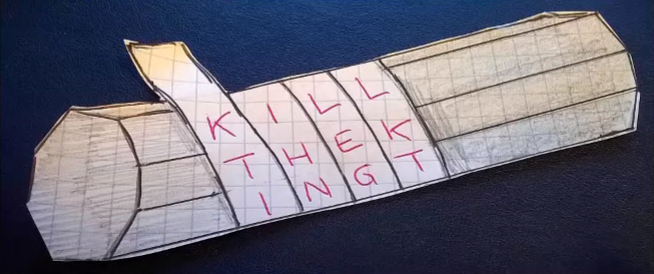
\includegraphics[scale=0.5]{2.png}
\end{center}
\subsection{Erodoto, Storie} Si tatuava il messaggio sulla testa rasata di un messaggero, si aspettava che ricrescessero i capelli e si portava a destinazione, rivelando il messaggio a seguito di una seconda rasatura.
\subsection{Enea Tattico}
Opera militare del IV secolo a.C. con un capitolo dedicato ai messaggi segreti. Consigliava di inviare un libro qualsiasi sottolineandovi un sottoinsieme di lettere che costituiscono il messaggio, oppure di sostituire le vocali di un testo con altri simboli grafici.
\subsection{Cifrario di Cesare}
Il più antico cifrario di concezione moderna. L'idea è che il crittogramma è ottenuto dal messaggio in chiaro sostituendo ogni lettera con quella di $3$ posizioni più avanti nell'alfabeto.\\
Non ha una chiave segreta, e la segretezza dipende dalla conoscenza del metodo: scoprire il metodo significa compromettere irrimediabilmente l'impiego. Il cifrario era quindi destinato all'uso ristretto di un gruppo di conoscenti.\\\\
Generalizzandolo a $k$ posizioni più avanti, si rende più sicuro ($1\leq k \leq 25$) e si ha $k$ come chiave segreta.
\subsubsection{Formulazione matematica}
Con pos(X) indichiamo la \textbf{posizione nell'alfabeto della lettera X}: ad esempio pos(A) = 0, pos(Z) = 25\ldots\\
La chiave $k$ è quindi $1 \leq k \leq 25$, con $k=26$ il cifrario lascerebbe invariato il messaggio.
\paragraph{Cifratura di X} Lettera Y $|$ pos(Y) = (pos(X) + $k$) mod 26
\paragraph{Decifrazione di Y} Lettera X $|$ pos(X) = (pos(Y) - $k$) mod 26\\\\
Un esempio con $k=10$. Cifriamo R, cui pos(R) = 17. La sua cifratura è (17+10) mod 26 = 1 = pos(B)\\Quindi R $\rightarrow$ B.
\subsubsection{Crittoanalisi}
\textbf{Se si conosce la struttura del cifrario}, in breve tempo \textbf{si possono applicare tutte le chiavi possibili}, che sono solo 25, ad un crittogramma: così viene \textbf{decifrato} e contemporaneamente si scopre la chiave segreta $k$.
Come cifrario risulta quindi inutilizzabile a fini crittografici.\\\\
\textbf{Gode della proprietà commutativa}: data una sequenza di chiavi e di operazioni di cifratura e decifrazione, l'\textbf{ordine delle operazioni può essere permutato arbitrariamente} senza modificare il crittogramma finale.\\
Per esempio, date $k_1$ e $k_2$ chiavi e $s$ sequenza,
\begin{list}{}{}
	\item C(C($s,k_2$),$k_1$) = C($s, k_1 + k_2$)
	\item D(D($s,k_2$),$k_1$) = D($s, k_1 + k_2$)
\end{list}
Una sequenza di operazioni di cifratura e decifrazione può essere ridotta ad una sola operazione di cifratura o decifrazione.\\\\
Inoltre \textbf{comporre più chiavi non aumenta la sicurezza} del sistema.
\section{Classificazione dei cifrari storici}
\subsection{Cifrari a sostituzione} Sostituiscono ogni lettera del messaggio in chiaro con una o più lettere dell'alfabeto secondo una regola prefissata.
\begin{list}{}{}
	\item \textbf{Sostituzione monoalfabetica} Es: Cifrario di Cesare.\\
	Alla stessa lettera del messaggio corrisponde sempre una stessa lettera nel crittogramma.\\
	Si possono impiegare funzioni di cifratura e decifrazione più complesse dell'addizione e della sottrazione in modulo, ottenendo uno spazio delle chiavi molto più ampio (ma sempre con una sicurezza molto modesta).\\\\
	Per esempio, usare come $k = \langle a,b \rangle$, cifrare pos(Y)=($a\cdot$pos(X)$+b)$ mod 26 e decifrare\\pos(X) = $a^{-1}\cdot($pos(Y)$-b)$ mod 26 con $a^{-1}$ inverso di $a$ mod 26 ($a\cdot a^{-1} = 1$ mod 26).\\
	C'è quindi un \textbf{vincolo forte} sulla chiave: MCD($a$, 26) $\neq$ 1 $\Rightarrow$ la funzione di cifratura non è iniettiva e la decifrazione diventa impossibile. Ad esempio con $k=\langle 13,0\rangle$ tutte le lettere posizione pari sono trasformate in A, mentre tutte quelle dispari sono trasformate in N.\\
	Le chiavi possibili sono quindi $12$ (scelte per $a$) $\cdot$ $26$ (scelte per $b$) = 312 chiavi che sono poche.\\\\
	Se la segretezza dipende unicamente dalla chiave, allora \textbf{il numero di chiavi deve essere così grande da essere praticamente immune dal brute force} e deve essere \textbf{scelta in modo casuale}.\\\\
	\textbf{Cifrario completo} prendendo una permutazione arbitraria dell'alfabeto come chiave:\\
\textit{lettera in chiaro in posizione $i$} $\longrightarrow$ \textit{lettera di posizione $i$ della permutazione}.\\\\
La chiave è di 26 lettere, con uno spazio delle chiavi esteso a $26! - 1$, cioè circa $4\cdot 10^{26}$ chiavi, il che lo rende molto vasto e inesplorabile.\\
Ma non è comunque sicuro: si può forzare senza ricorre a brute force, sfruttando la struttura logica dei messaggi in chiaro e l'occorrenza statistica delle lettere.
	\item \textbf{Sostituzione polialfabetica}\\
	Alla stessa lettera del messaggio corrisponde una lettera scelta in un insieme di lettere possibili, secondo una regola opportuna (a seconda della posizione o del contesto in cui appare la lettera nel messaggio). L'esempio più antico è l'archivio cifrato di Augusto.\\
	I documenti in archivio erano scritti in numeri, invece che lettere. Augusto li scriveva in greco, poi metteva in corrispondenza la sequenza di lettere del documento con la sequenza di lettere del primo libro dell'Iliade. Sostituiva ogni lettera del documento con il numero che indicava la distanza, nell'alfabeto greco, di tale lettera con quella in pari posizione nell'Iliade.\\
	Per esempio:
	\begin{list}{}{}
		\item Lettera in posizione $i$ nel documento: $\alpha$
		\item Lettera in posizione $i$ nell'Iliade: $\epsilon$
		\item Carattere in posizione $i$ nel crittogramma: 4 (distanza tra $\alpha$ e $\epsilon$)
	\end{list}
	Se la chiave è lunghissima, il cifrario diventa difficile da forzare. Venne usato anche della Seconda Guerra Mondiale, prendendo come chiave una pagina prefissata di un libro e cambiandola di giorno in giorno. Lo \textbf{svantaggio} è \textbf{registrare per iscritto la chiave}.\\\\
	\textbf{Cifrario di Alberti} con due dischi, dove si cambia chiave ogni volta che si incontra un carattere speciale. Inserendo spesso caratteri speciali (scartati nel messaggio ricostruito) diventa difficile da attaccare e il continuo cambio di chiave rende inutili gli attacchi basati sulla frequenza dei caratteri. La \textbf{Macchina Enigma} è un'\textbf{estensione elettromeccanica del cifrario di Alberti}.\\\\
	\textbf{Cifrario di Vigenère}, con una parola segreta $k$ come chiave. La cifratura di un messaggio $m$ avviene disponendo $m$ e $k$ su due righe adiacenti, allineando le lettere in verticale (se $k$ è più corta di $m$ la si ricopia più volte). Ogni lettera X di $m$ risulta allineata ad una lettera $Y$ della chiave. La X è sostituita nel crittogramma con la lettera che si trova nella cella T all'incrocio tra la riga che inizia con X  e la colonna che inizia con Y
	\begin{center}
		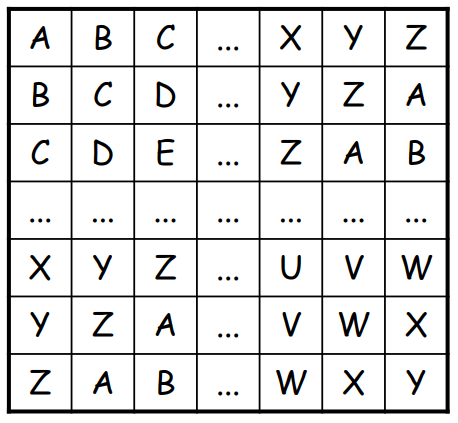
\includegraphics[scale=0.5]{6.png}
	\end{center}
	Quindi le lettere allineate con A non subiscono modifiche. Quelle allineate con B sono traslate di una posizione in avanti, quelle con R di 17 posizioni\ldots\\
	Una stessa lettera in chiaro è cifrata in modi diversi a seconda della lettera con cui è allineata, mentre per la decifrazione si esegue il processo inverso.\\
	La sicurezza del metodo è influenzata dalla lunghezza della chiave: se contiene $h$ caratteri, le apparizioni della stessa lettera distanti un multiplo di $h$ nel messaggio si sovrappongono alla stessa lettera della chiave, quindi sono trasformate nella stessa lettera cifrata.\\
	I cifrari polialfabetici non sono molto più potenti dei monoalfabetici se le chiavi non sono molto lunghe.\\
	Se si estende Vigenèere impiegando una chiave lunga quanto il testo, casuale e non riutilizzabile, il cifrario diventa inattaccabile: \textbf{one-time pad}.
\end{list}
\subsection{Cifrari a trasposizione} Permutano le lettere del messaggio in chiaro secondo una regola prefissata.\\
L'idea di base è eliminare qualsiasi struttura linguistica presente nel crittogramma: permutando le lettere del messaggio in chiaro e inserendone eventualmente altre ignorate nella decifrazione.
\paragraph{Semplice} La chiave è un intero $h$ e una permutazione $\pi$ degli interi $\{1,2,\ldots,h\}$\\
Nella cifratura si suddivide il messaggio in $m$ blocchi da $h$ lettere e si permutano le lettere di ciascun blocco secondo $\pi$.\\
Se la lunghezza di $m$ non è divisibile per $h$, si aggiungono alla fine delle lettere qualsiasi (padding): partecipano alla trasposizione, ma sono ignorate perché la decifrazione le riporta alla fine del messaggio.\\
Ci sono $h! -1$ chiavi ed $h$ non è fissato a priori: tanto è più grande tanto è più difficile impostare un brute force. Al crescere di $h$ però cresce anche la difficoltà di ricordare $\pi$.
\paragraph{Permutazione di colonne} $k=\langle c,r,\pi\rangle$ con:\begin{list}{}{}
	\item $c$ ed $r$ denotano il numero di colonne e righe di una tabella di lavoro $T$
	\item $\pi$ è una permutazione degli interi $\{1,2,\ldots,c\}$
\end{list}
Il messaggio $m$ è decomposto in blocchi $m_1,m_2\ldots$ di $c\cdot r$ caratteri.\\
Nella cifratura i caratteri di ogni blocco sono distribuiti tra le celle di T in modo regolare, scrivendoli per righe dall'alto verso il basso. Poi le colonne vengono permutate secondo $\pi$ e si prendono le colonne dalla prima leggendole dall'alto verso il basso e da sinistra verso destra, ottenendo il crittogramma.
\begin{center}
	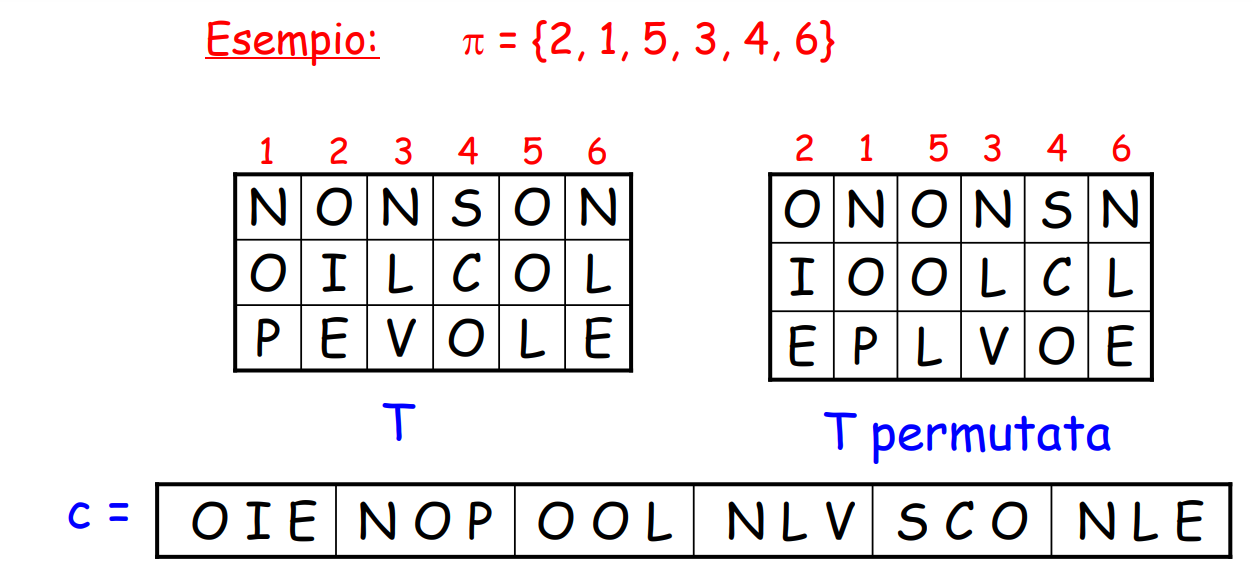
\includegraphics[scale=0.4]{7.png}
\end{center}
Per cifrare il prossimo blocco, si azzera T e si ripete il procedimento.\\
Le chiavi sono teoricamente esponenziali nella lunghezza del messaggio, non essendoci vincoli su $r$ e $c$.
\paragraph{Cifrario a griglia} Antenato: cifrario di Richelieu. Il crittogramma può essere celato in un libro qualsiasi. La chiave è data da una scheda perforata e dall'indicazione di una pagina del libro: la decifrzione consiste nel sovrapporre la scheda alla pagina, e le lettere visibili attraverso i fori costituiscono il messaggio in chiaro.
\section{Crittoanalisi Statistica} La sicurezza di un cifrario è legata alla dimensione dello spazio delle chiavi. Ci sono altri metodi di attacco: i cifrari storici sono stati violati con un attacco statistico di tipo cipher text.\\
Nella crittoanalisi statistica si fanno delle ipotesi. Ci sono delle \textbf{informazioni note al crittoanalista}: il metodo usare per la cifratura e la decifrazionem, il linguaggio naturale con cui è scritto il messaggio e si ammette che il messaggio sia sufficientemente lungo per poter rilevare alcuni dati statistici sui caratteri che compongono il crittogramma.
\paragraph{Attacco} La frequenza con cui appaiono in media le varie lettere dell'alfabeto è ben studiata in ogni lingua. Dati simili sono noti per le frequenze di diagrammi (gruppi di due lettere consecutive), trigrammi (gruppi di tre lettere) e così via (\textbf{q-grammi}).
\paragraph{Decifrazione cifrari monoalfabetici}
Se un crittogramma è generato per sostituzione monoalfabetica allora la frequenza di Y nel crittogramma è circa la frequenza della corrispondente X del messaggio.\\
Nei \textbf{cifrari completi} si associano le lettere in base alle frequenze, provando le varie combinazioni. Con le combinazioni di prova, si studiano le frequenze dei possibili diagrammi, dei trigrammi e così via.
\paragraph{Decifrazione cifrari polialfabetici} Più difficile. Per esempio in Vigenère ogni lettera Y del crittogramma dipende da una coppia di lettere $\langle$X, K$\rangle$ provenienti dal messaggio e dalla chiave.\\
Se la chiave è di $h$ caratteri, il crittogramma è composto di $h$ sottosequenze, ciascuna ottenuta per sostituzione monoalfabetica. Il problema è scoprire $h$ per scomporre il crittogramma e continuare la decifrazione con il metodo monoalfabetico.\\
Quindi il messaggio contiene quasi sicuramente gruppi di lettere adiacenti ripetuti più volte. Le apparizioni della stessa sottosequenza allineate con la stessa porzione di chiave danno sottosequenze identiche. Si cercano nel crittogramma coppie di posizioni $p_1$, $p_2$ in cui indiziano sottosequenze identiche. La distanza $d = p_2 - p_1$ è \textit{probabilmente} uguale ad $h$ o ad un suo multiplo.
\paragraph{Decifrazione di cifrari a trasposizione}
Le lettere nel crittogramma sono le stesse del messaggio in chiaro, non ha senso un attacco statistico basato sulle frequenze: si studiano i q-grammi\\
Se si conosce la lunghezza $h$ della chiave, si divide il crittogramma in porzioni di lunghezza $h$, in ciascuna si cercano gruppi di $q$ lettere che formano i q-grammi più diffusi. se un gruppo deriva effettivamente da un q-gramma, si scopre parte della permutazione.
\paragraph{Conclusione} La rilevazione delle frequenze delle singole lettere del crittogramma è un potente indizio per discernere tra i vari tipi di cifrario:
\begin{list}{}{}
	\item nei cifrari a trasposizione, l'istogramma delle frequenze coincide circa con quello proprio del linguaggio
	\item nei cifrari a sostituzione monoalfabetica, i due istogrammi coincidono a meno di una permutazione delle lettere
	\item nei cifrari a sostituzione polialfabetica, l'istogramma del crittogramma è assai più appiattito di quello del linguaggio
\end{list}
\section{La Macchina Enigma} \paragraph{Automatismo} Prima evoluzione verso i sistemi automatizzati, la \textbf{macchina Enigma} ha avuto un ruolo fondamentale nella seconda guerra mondiale. Ci sono stati \textbf{molti studi dedicati a comprometterne la sicurezza}, che hanno posto le \textbf{fondamenta per la nascita dei calcolatori odierni}.\\
Fu inventata in Germania nel 1918 per applicazioni commerciali, come estensione elettromeccanica del cifrario di Alberti.
\paragraph{Rotori} La macchina era composta da rotori, una tastiera, una griglia di luci sopra la tastiera corrispondenti alle lettere (lampboard) e una plugboard inferiore.\\
I rotori \textbf{non mantenevano la stessa posizione reciproca durante la cifratura}. Per ogni lettera battuta sulla tastiera:
\begin{list}{}{}
	\item Il primo rotore avanzava di un passo
	\item Dopo 26 passi (\# di lettere), il primo rotore era tornato sulla posizione iniziale e il secondo rotore avanzava di un passo
	\item Dopo una rotazione completa del secondo rotore, il terzo rotore avanzava di un passo.
\end{list}
Questo fa si che la corrispondenza tra caratteri cambiasse ad ogni passo, cioè \textbf{la chiave cambiava ad ogni lettera premuta}: $26\cdot26\cdot26 = 17476$ chiavi diverse.
\paragraph{Debolezza} I rotori erano immutabili, inoltre le $26^3$ permutazioni sono sempre le stesse, applicate nello stesso ordine e note a tutti i proprietari di una macchina Enigma.\\
Alberti prevedeva, per ogni coppia di utenti, una coppia di dischi diversa da tutte le altre.
\paragraph{Modifiche} Possibilità di permutare tra loro i tre rotori: \# permutazioni = $3!\cdot26^3 > 10^5$\\
Inoltre fu aggiunta la plugboard fra la tastiera e il primo rotore: consente di \textbf{scambiare fra loro i caratteri di 6 coppie scelte arbitrariamente in ogni trasmissione}. Ogni cablaggio è descritto da una sequenza di 12 caratteri (le 6 coppie da scambiare): $\left(\begin{array}{c}26\\12\end{array}\right)\simeq 10^7$ combinazioni possibili. Ogni gruppo di 12 caratteri può presentarsi in $12!$ permutazioni diverse, ma non tutte producono effetti diversi: ad esempio \textsc{ab cd ef gh ij kl} e \textsc{cd ab ef gh ij kl} producono lo stesso effetto, e con queste anche tutte le $6!$ permutazioni delle 6 coppie.\\
Infine vanno considerati i possibili scambi tra gli elementi delle coppie che producono lo stesso effetto:\\\textsc{ab cd ef gh ij kl} e \textsc{ba cd ef hg ij kl} ad esempio, quindi dobbiamo dividere per un ulteriore fattore $2^6 = 64$
\paragraph{Numero di chiavi} Il numero di chiavi dei rotori ($> 10^5$) si moltiplica per un fattore $\left(\begin{array}{c} 26\\12\end{array}\right)\frac{12!}{6!\cdot64} > 10^{11}$\\
per un totale di più di $10^{16}$ chiavi (10 \textit{milioni di miliardi} di combinazioni possibili)
\paragraph{Seconda Guerra Mondiale} 8 rotori in dotazione, da cui sceglierne 3, e 10 coppie scambiabili tramite plugboard.\\
Elenco di chiavi giornaliere in dotazione ai reparti militari, cioè l'assetto iniziale della macchina per quel giorno. Con quell'assetto, si trasmetteva una nuova chiave di messaggio, che indicava l'assetto da usare per quella particolare trasmissione.
\paragraph{Storia di Enigma} Era lo standard militare tedesco durante la seconda guerra mondiale. Matematici polacchi e inglesi studiarono come rompere il cifrario (\textbf{Bletchley Park}): era necessaria una \textbf{rapida decifrazione} perché il sistema è continuamente variato.
\begin{list}{}{}
	\item Costruzione di un simulatore di Enigma per studiarne il comportamento sotto possibili variazioni.\\
	Alan Turing e altri.
	\item Macchina COLOSSUS\\
	1944
	\item Prototipo embrionale dei successivi calcolatori elettronici.
\end{list}
\chapter{Cifrari perfetti}
Shannon, 1949
\paragraph{Cifrario perfetto} Sono cifrari che ci offrono una \textbf{sicurezza incondizionata}, proteggono le informazioni con certezza assoluta indipendentemente dalla potenza di calcolo. Si rende \textbf{essenziale avere la chiave}, un'attacco \textbf{brute force non permette di decifrare}.\\
Informalmente, un cifrario è perfetto se la \textbf{sicurezza è garantita qualunque sia l'informazione carpita dal canale di comunicazione}.\\
Abbiamo quindi due spazi:
\begin{list}{}{}
	\item MSG: lo \textbf{spazio dei messaggi}
	\item CRITTO: lo \textbf{spazio dei crittogrammi}
\end{list}
e due variabili aleatorie:
\begin{list}{}{}
	\item M: descrive il \textbf{comportamento del mittente}, con valori in MSG
	\item C: descrive il \textbf{processo di comunicazione}, con valori in CRITTO
\end{list}
Ho delle probabilità:
\begin{list}{}{}
	\item P(M = $m$): probabilità che il mittente voglia spedire il messaggio $m$
	\item P(M = $m$ $|$ C = $c$): probabilità condizionata che il messaggio inviato sia $m$ posto che sul canale stia transitando il crittogramma $c$
\end{list}
Con $\forall$ $m\in$ MSG e $\forall$ $c\in$ CRITTO.\\
Scenario: il crittoanalista conosce tutto del sistema tranne la chiave, quindi conosce:
\begin{list}{}{}
	\item la distribuzione di probabilità con cui il mittente invia i messaggi
	\item cifrario utilizzato
	\item lo spazio delle chiavi (KEY)
\end{list}
\paragraph{Definizione} Un cifrario è perfetto se $\forall$ $m\in$ MSG e $\forall$ $c\in$ CRITTO, allora P(M = $m$) = P(M = $m$ $|$ C = $c$), cioè la conoscenza di $c$ non raffina la conoscenza.
%TODO esempi
In un cifrario perfetto, la conoscenza del crittoanalista non cambia dopo che è stato osservato un crittogramma in transito. Quindi \textbf{il messaggio ed il crittogramma appaiono del tutto scorrelati, nessuna informazione sul messaggio filtra dal crittogramma}.
\subsection{Teorema di Shannon} In un cifrario perfetto il numero delle chiavi deve essere maggiore o uguale del numero dei messaggi possibili (cioè con probabilità non nulla di essere inviati)
\paragraph{Dim} Per assurdo
\begin{list}{}{}
	\item $N_m$ = \# dei messaggi possibili, cioè $m\in$ MSG $|$ P(M = $m$) $>$ 0
	\item $N_k$ = \# delle chiavi
\end{list}
\pagebreak
Suppongo per assurdo che $N_k < N_m$. Suppongo $c\in$ CRITTO con P(C = $c$) $>$ 0. Conto i messaggi che possono corrispondere al crittogramma $\Rightarrow$ $s$ messaggi potenzialmente corrispondenti a $c$. Questi $s$ messaggi sono i messaggi che posso ottenere decifrando $c$ con ogni chiave possibile: con la chiave $k_1$ ottengo $m_1$, $k_2$ ottengo $m_2$, ma anche possibile che con $k_3$ ottenga di nuovo $m_2$ dato che non so come funziona il cifrario. Posso dire con certezza che $s \leq N_k$ e per ipotesi $N_k < N_m$\\
Ottengo $s < N_m$ $\Rightarrow\:\exists\:m\in$ MSG con P(M = $m$) $>$ 0 $|$ P(M = $m$ $|$ C = $c$) = 0, ottenendo una conoscenza maggiore (posso escludere $m$) quindi il cifrario non è perfetto, ottenendo una \textbf{contraddizione}.
\subsection{One-Time Pad}
1917, Mauborgne, Vernam\\
Usa l'alfabeto binario \{0,1\}, usato sia durante le guerre mondiali che durante la guerra fredda. L'idea è avere una chiave lunghissima consumata man mano e mai riutilizzata.\\
MSG, CRITTO e KEY sono spazi di sequenze binarie. La regola è pubblica e usa lo xor. Quindi sia C che D usano lo xor (somma in modulo 2) per trasformare il messaggio nel crittogramma e viceversa.\\
$m\in\{0,1\}^n$ e $k\in\{0,1\}^n$ con $n > 0$ fissato.\\
$c = C(m, k) = m \oplus k$
Con $n=5$, $m=10110$, $k=01011$ allora $c=11101$.\\La decifrazione $m = D(c,k) = c \oplus k = (m\oplus k)\oplus k) = m \oplus (k \oplus k) = m$ perché $k \oplus k = 0\ldots 0$\\
\textbf{Fondamentale non riutilizzare la chiave}. Questo perché avendo $c', c''$ ottenuti con la stessa $k$ da $m',m''$, faccio $c'\oplus c'' = (m'\oplus k) \oplus (m''\oplus k) = m'\oplus m'' \oplus (k \oplus k) = m' \oplus m''$, acquisendo conoscenza (lunghi tratti di 0 significa tratti uguali nei messaggi in chiaro).
\paragraph{Teorema} Quando il One-Time Pad è perfetto. Ipotesi:
\begin{enumerate}
	\item Tutti i messaggi hanno lunghezza $n$, con del padding o divisione in blocchi all'occorrenza
	\item Tutte le sequenze di $n$ bit sono messaggi possibili (per quelle prive di senso probabilità molto bassa ma comunque $> 0$)
	\item Chiave scelta \textbf{perfettamente a caso per ogni messaggio}
\end{enumerate}
Il \textbf{teorema} dice che sotto 1, 2 e 3 One-Time Pad è \textbf{un cifrario perfetto e minimale} (usa un numero minimo di chiavi)
\subparagraph{Dim} Dimostro che è perfetto, cioè che $\forall$ $m\in$ MSG e $\forall$ $c\in$ CRITTO, allora P(M = $m$) = P(M = $m$ $|$ C = $c$)\\
P(M = $m$ $|$ C = $c$) = $\frac{P(M = m \wedge C = c)}{P(C = c)}$ = $\frac{P(M = m)\cdot P(C = c)}{P(C = c)}$ = P(M = $m$)\\
Per le proprietà dello xor, fissato $m$ chiavi diverse producono crittogrammi diversi $\Rightarrow$ $\exists!$ chiave $k$ $|$ $m\oplus k = c$
$\forall\:c\in$ CRITTO, P(C = $c$) = P(scegliere l'unica chiave $k$ $|$ $m\oplus k = c$) = $\frac{1}{2^n}$, questo perché \{M = $m$\} e \{C = $c$\} sono \textbf{eventi indipendenti}.\\
Per quanto riguarda la minimalità, cioè $N_k \geq N_m$, il One-Time Pad per ogni $n$ ha $N_k = N_m = N_{CRITTO} = 2^n$, questo perché anche le chiavi sono sequenze di $n$ bit come i messaggi e i crittogrammi.
\paragraph{Attacchi}
\begin{list}{}{}
	\item Bruteforce: non ha senso, ogni chiave fa ricostruire un messaggio possibile quindi non aggiunge conoscenza
\end{list}
Rimane il problema di generare le sequenze di bit completamente casuali.
\paragraph{Osservazione} Rimuoviamo la seconda ipotesi nella dimostrazione. Per esempio in inglese i messaggi significativi sono circa $\alpha^n << 2^n$ con $\alpha = 1.1$\\
Quindi $N_m = \alpha^n$, $N_k\geq N_m$ cioè $N_k\geq \alpha^n$, la chiave sarà una sequenza di $t$ bit con $t$ $|$ $2^t \geq \alpha^n$\\
Risolvo trovando $t \geq \log_w \alpha^n = n \log_2 \alpha = 0.12\cdot n$\\\\
Per confondere l'avversario è opportuno che coppie diverse $(m,k)$ producano lo stesso crittogramma $\Rightarrow$ \# coppie $(m,k) >>$ \# crittogrammi, cioè $\alpha^n 2^t >> 2^n$
\pagebreak
\section{Principi di Shannon}
Principi per la resistenza agli attacchi di crittoanalisi statistica:
\begin{list}{}{}
	\item \textbf{Diffusione}: tutti i caratteri del testo in chiaro si devono spargere nel crittogramma.
	\item \textbf{Confusione}: combinare testo in chiaro e chiave in modo complesso, per non permettere al crittoanalista di sapere le due sequenze analizzando il crittogramma.
\end{list}
\paragraph{Standard} 1972 NBS (National Bureau of Standards) $\rightarrow$ 1973 NIST (National Institute for Security and Technology)
\begin{list}{}{}
	\item \textbf{Sicurezza basata sulla segretezza della chiave} e non sul processo di cifratura e decifrazione (che è \textbf{pubblico})
	\item \textbf{Algoritmo efficiente} in software e hardware
\end{list}
IBM propone \textbf{LUCIFER}, poi migliorato con l'NSA. Da 128 bit a 56 bit per la chiave: variazioni nella s-box.\\
Si arriva al 1977 con il \textbf{DES}, accettato e reso pubblicamente disponibile (licenza d'uso gratuita): \textbf{Data Encryption Stantard}. Rimane fino al 1999, quando si sconsiglia il DES in favore del 3DES. Dal 2005 anche il 3DES risulta superato, al suo posto \textbf{AES} (\textbf{Advanced Encryption Standard})
\section{Data Encryption Standard}
Cifratura a blocchi di 64 bit e chiave segreta di 64 bit: 56 bit casuali e 8 bit di parità suddivisi in: 7 bit, bit parità, 7 bit, bit parità\ldots\\
$r = 16$ fasi in cui si ripetono le stesse operazioni.
\begin{multicols}{2}
	\begin{center}
		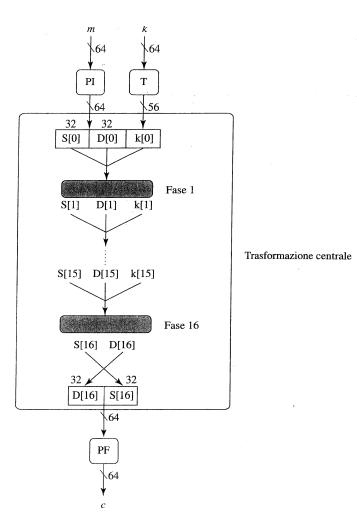
\includegraphics[scale=0.75]{8.png}
	\end{center}
	\columnbreak
	\paragraph{Struttura del DES}
	\begin{list}{}{}
		\item $m$: blocco del messaggio
		\item $c$: corrispondente blocco del crittogramma
		\item $k$: chiave segreta con i bit di parità
		\item
		\item $\forall\:i=1,\ldots,16$ ho
		\begin{list}{}{}
			\item $S[i] = D[i-1]$
			\item $D[i] = S[i-1]\oplus f(D[i-1], k[i-1])$\\
			$f$: funzione \textbf{non} lineare
		\end{list}
	\end{list}
\end{multicols}
\pagebreak
\paragraph{Fase $i$-esima del DES}
\begin{center}
	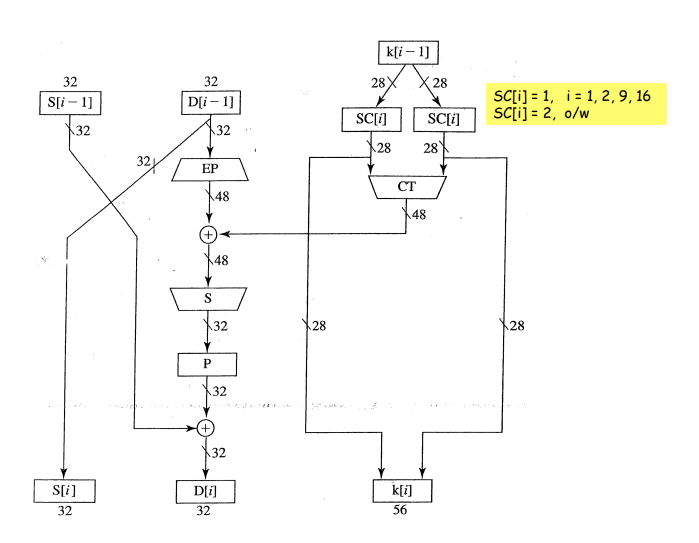
\includegraphics[scale=0.75]{9.png}
\end{center}
\paragraph{Permutazioni}
\begin{center}
	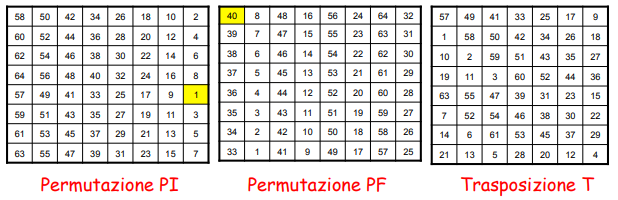
\includegraphics[scale=0.75]{10.png}
\end{center}
Le tabelle vanno lette per righe.
\begin{list}{}{}
	\item \textbf{Permutazione PI}: riordina i bit del messaggio $m = m_1 m_2\ldots m_{64}$ come $m_{58} m_{50}\ldots m_7$: ad esempio porta in posizione 40 (numero della cella) il bit in posizione 1 (contenuto della cella)
	\item \textbf{Permutazione PF}: è l'inversa di PI, cioè nell'esempio riporta in posizione 1 il bit in posizione 40
	\item \textbf{Trasposizione T}: provvede anche a scartare dalla chiave $k = k_1 k_2\ldots k_{64}$ i bit di controllo $k_8, k_16, \ldots k_64$, generando una sequenza di 56 bit che costituisce la prima sottochiave $k[0]$
\end{list}
\pagebreak
\paragraph{Funzioni CT e EP}
\begin{center}
	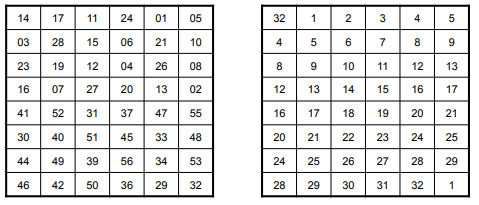
\includegraphics[scale=0.75]{11.png}
\end{center}
\begin{list}{}{}
	\item \textbf{Funzione CT}: 8 bit dell'ingresso (es: il bit 9) non sono presenti in uscita
	\item \textbf{Funzione EP}: 16 bit di ingresso sono duplicati (es: il bit 32 è copiato nelle posizioni 1 e 47 dell'uscita)
\end{list}
\paragraph{S-box}
\begin{center}
	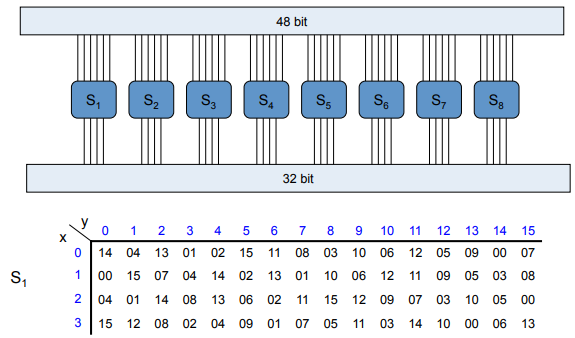
\includegraphics[scale=0.75]{12.png}
\end{center}
Tabella che definisce la sottofunzione $S_1$. Le sottofunzioni $S_2,\ldots,S_8$ sono definite in modo simile.
\begin{center}
	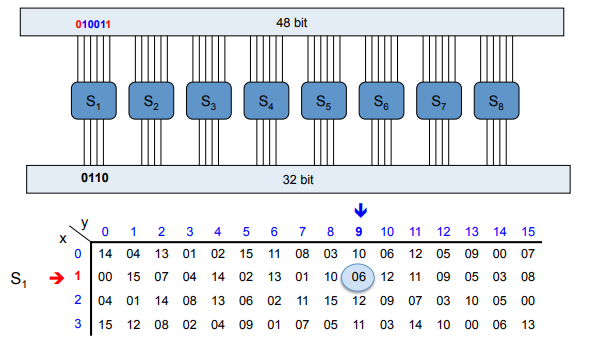
\includegraphics[scale=0.75]{13.png}
\end{center}
\pagebreak
\paragraph{Permutazione P}
\begin{center}
	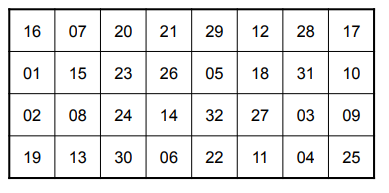
\includegraphics[scale=0.75]{14.png}
\end{center}
Permutazione di 32 bit che genera il blocco finale $D[i]$.
\paragraph{Attacchi} Due metodi principali:
\begin{enumerate}
	\item Architetture apposite progettate per attaccare il DES
	\item Calcolo distribuito su più macchine
\end{enumerate}
\subparagraph{Attacchi esaurienti}
\textbf{Chosen Plain Text}: il crittoanalista si procura coppie $\langle m, c_1\rangle, \langle \overline{m}, c_2\rangle$\\
Da $C(m, k)$ = $\begin{array}{l}
	c_1 \Rightarrow k \textsl{ probabile chiave}\\
	c_2 \Rightarrow \overline{k} \textsl{ probabile chiave}
\end{array}$
\subparagraph{Crittoanalisi differenziale} $2^{47}$ coppie $\langle m,c\rangle$ scelti dal crittoanalista. L'attacco costa complessivamente $2^{55}$ con $r=16$.
\subsection{Varianti del DES}
\paragraph{Scelta indipendente delle sottochiavi di fase} \# bit 56 $\rightarrow$ 16$\cdot$48 = 768 bit\\
Crittoanalisi differenziale $\rightarrow$ 2$^{61}$
\paragraph{Cifratura multipla} $\forall\:k_1,k_2$ ho $C_D(C_D(n, k_1), k_2) \neq C_D(n, k_3)$, questo $\forall\:n, k_3$\\
\# spazio delle chiavi = 2$^{112}$, non sono 112 bit di sicurezza\\ %TODO riascoltare lezione
Sicurezza pari a quella di una chiave da 57 bit
\subparagraph{Attacco "Meet in the Middle"} $c$ = C(C($n, k_1$), $k_2$), con $k_1,k_2$ chiavi di 56 bit $\rightarrow$ D($c, k_2$) = C($n, k_1$)\\
Si prende una coppia $\langle n,c\rangle$
\begin{list}{}{}
	\item $\forall\:k_1$ calcolo e salvo C($n, k_1$) (2$^{56}$)
	\item $\forall\:k_2$ calcolo D($c, k_2$) e lo cerco nella lista delle cifrature\\
	Deve \textbf{esistere certamente almeno una corrispondenza} ($N$ = 2$^{56}$)
	\item N = $2^{56}$ cifrature + O(N) decifrazioni\\
	Quindi costo 2N $<<$ N$^2$ (costo dell'enumerazione di tutte le coppie ($k_1, k_2$))
\end{list}
\paragraph{3DES} TDEA = Trple Data Encryption Algorithm\\
2TDEA, 3TDEA: 2 e 3 sono \# chiavi\begin{list}{}{}
	\item \textbf{2TDEA}\\
	$c$ = C(D(C($n, k_1$), $k_2$), $k_1$), con $k_1, k_2$ chiavi di 56 bit tra loro indipendenti.\\
	$k_1 = k_2 \Rightarrow$ 2TDEA equivale ad una singola cifratura DES. CDC non è più robusto di CCC, 112 bit di sicurezza.
	\item \textbf{3TDEA}\\
	$c$ = C(D(C($n, k_1$), $k_2$), $k_3$), con $k_1, k_2, k_3$ chiavi di 56 bit tra loro indipendenti.\\
	\# bit della chiave: 56$\cdot$3 = 168 bit\\
	Vulnerabile a meet in the middle $\rightarrow$ 112 bit di sicurezza\\\pagebreak\\
	$m = D(C(D(c, k_3), k_2) k_1) \Rightarrow C(m, k_1) = C(D(c, k_3), k_2)$
	\begin{enumerate}
		\item Enumero le chiavi di 56 bit e salvo la lista C$(m, k_1)$ $\forall\:k_1 \in \{0, 1\}^{56}$
		\item $\forall\:k_2, k_3$ calcolo $C(D(c, k_3), k_2)$ e lo cerco nella lista\\
		$2^{56} + 2^{112}$, $2^{56}$ dal punto 1 e $2^{112}$ costo di enumerazione delle coppie $k_2, k_3$
	\end{enumerate}
\end{list}
\paragraph{AES} 128 bit di chiave\\
Ogni sottochiave di fase, $w(i)$, è una sequenza di 4 byte che usa la s-box.\\
$k = \begin{tabular}{|c|c|c|c|}
\hline
 & & & 1byte \\
\hline
 & & & \\
\hline
 & & & \\
\hline
 & & & \\
\hline
\multicolumn{1}{c}{w(0)} & \multicolumn{1}{c}{w(1)} & \multicolumn{1}{c}{w(2)} & \multicolumn{1}{c}{w(3)}\\
\end{tabular}$\\
Chiave: $w(0), w(1), w(2), w(3)$\\
$\forall\:t\geq 4$ ho $w(t) = \left\{\begin{array}{l l}
w(t-1)\oplus w(t-4) &\textsl{se }4\not|\:t\\
T(w(t-1))\oplus w(t-4) &\textsl{se }4\:\:|\:t
\end{array}\right.$ con $T$ non lineare e che usa la s-box\\\\
Chiave alla $i$-esima fase, $1\leq i \leq 10$: $w(4i), w(4i + 1), w(4i + 2), w(4i + 3)$
\subparagraph{Cifratura} Blocchi di 128 bit, riempita per colonne $b_{ij} \in \{0, 1\}^8$\\
$B = \left[\begin{array}{c c c c}
b_{00} & b_{01} & b_{02} & b_{03} \\
b_{10} & b_{11} & b_{12} & b_{13} \\
b_{20} & b_{21} & b_{22} & b_{23} \\
b_{30} & b_{31} & b_{32} & b_{33} \\
\end{array}\right]$\\
Trasformazione iniziale: $k$ matrice della chiave, con $B$ costruisco $B\oplus k$\\
10 fasi da 4 operazioni:
\begin{list}{}{}
	\item[01] \texttt{SUBISTITUTE BYTES}\\
	Ogni byte di $B$ è trasformato usando s-box: $b_{ij} \rightarrow$ s-box$(b_{ij})$
	\item[02] \texttt{SHIFT ROWS}
	\item[03] \texttt{MIX COLUMNS}, non si applica nella fase 10
	\item[04] \texttt{ADD ROUND KEY}
	\item Alla fine delle 10 fasi, il blocco B è il crittogramma
\end{list}
\subparagraph{S-box} Matrice 16$\times$16 di interi $\in(0, 255) \Rightarrow$ contiene una permutazione\\
$b_{ij} \rightarrow$ s-box$(b_{ij})\in\{0,1\}^8$\\
$b_{ij} = b_1b_2b_3b_4|b_5b_6b_7b_8$
\begin{list}{}{}
	\item Riga: $b_1b_2b_3b_4$, $0\leq x \leq 15$
	\item Colonna: $b_5b_6b_7b_8$, $0\leq y \leq 15$
\end{list}
Es $b_{ij} = 1000|1011$ = $8|11$, s-box$[8, 11] \rightarrow 61$ cioè $00111101$\\\\
$x$ byte $\longrightarrow_{s-box}$ $x^{-1}$ inverso moltiplicativo + composizione lineare in GF($2^8$)\\
Galois Field, campi finiti di Galois
\begin{list}{}{}
	\item[02] \texttt{SHIFT ROWS}\\
	$\begin{array}{c c c c}
\underline{b_{00}} & b_{01} & b_{02} & b_{03} \\
\underline{b_{10}} & b_{11} & b_{12} & b_{13} \\
\underline{b_{20}} & b_{21} & b_{22} & b_{23} \\
\underline{b_{30}} & b_{31} & b_{32} & b_{33} \\
\end{array} \rightarrow \begin{array}{c c c c}
\underline{b_{00}} & b_{01} & b_{02} & b_{03} \\
b_{11} & b_{12} & b_{13} & \underline{b_{10}} \\
b_{22} & b_{23} & \underline{b_{20}} & b_{21} \\
b_{33} & \underline{b_{30}} & b_{31} & b_{32} \\
\end{array}$
	\item[03] \texttt{MIX COLUMNS}\\
	$M$ matrice di $4\times 4$ byte. Ogni colonna del blocco B 
	$B_j \rightarrow M\cdot B_j$, con $0 \leq j \leq 3$\\
	Il nuovo $b_{ij}$ diventa un valore che dipende da tutti i byte della colonna ($b_{0j}, b_{1j}, b_{2j}, b_{3j}$)\\
	$b_{ij} \rightarrow b_{ij}\oplus k_{ij}$
\end{list}

\chapter{Crittografia a Chiave Pubblica}
Cifrari ibridi, usati per lo \textbf{scambio delle chiavi}.
\paragraph{One-Time Pad} 1917\\
Non può essere decifrato senza conoscere la chiave. \textbf{Assolutamente sicuro}, ma richiede una nuova chiave segreta per ogni messaggio, che deve essere perfettamente casuale e lunga quanto il messaggio da scambiare. Diventa molto attraente per chi richiede una sicurezza assoluta ed è disposto a pagarne i costi.\\
Ma \textbf{come si genera} e \textbf{come si scambia la chiave}?
\section{AES} \paragraph{Advanced Encryption System} Standard per le comunicazioni riservate ma non-classificate. Pubblicamente noto e realizzabile su hardware di ogni tipo, con chiavi brevi (128/256 bit, qualche decina di caratteri)\\
Ma come scambiare in sicurezza una chiave segreta? La chiave serve per comunicare in sicurezza, ma deve essere stabilita comunicando \textit{in sicurezza} senza poter ancora usare il cifrario.
\subsection{Protocollo DH} Nel 1976 viene proposto un algoritmo per generare e scambiare una chiave segreta su un canale insicuro, senza necessità che le due parti si siano scambiate informazioni o incontrate in precedenza. Il \textbf{protocollo DH} è un algoritmo ancora usato nei protocolli crittografici su Internet. Diffie e Hellman propongono anche la definizione di crittografia a chiave pubblica, ma senza avere un'implementazione pratica.
\subsection{Cifrari simmetrici} Nei \textbf{cifrari simmetrici}, la \textbf{chiave di cifratura è uguale a quella di decifrazione} (o l'una può essere facilmente calcolata dall'altra) ed è \textbf{nota solo ai due partner} che la scelgono di comune accordo e la mantengono \textbf{segreta}.
\subsection{Cifrari asimmetrici} Nei \textbf{cifrari a chiave pubblica} l'\textbf{obiettivo} è \textbf{permettere a tutti di inviare messaggi cifrati ma abilitare solo il ricevente} (Bob) \textbf{a decifrarli}.\\
Le \textbf{operazioni di cifratura e decifrazione sono pubbliche} e usano \textbf{due chiavi diverse}:
\begin{list}{}{}
	\item $k_{pub}$ per \textbf{cifrare}: \textbf{pubblica}
	\item $k_{priv}$ per \textbf{decifrare}: \textbf{privata}, nota solo a Bob
\end{list}
Esiste una coppia $\langle k_{pub}, k_{priv}\rangle$ per ogni utente del sistema, scelta da questi nella sua veste di possibile destinatario.
\paragraph{Cifratura} La \textbf{cifratura di un messaggio da spedire} a Bob è eseguita da qualunque mittente come $$c = C(m, k_{pub})$$ La chiave $k_{pub}$ e la funzione di cifratura $C(m, k)$ sono note a tutti.
\paragraph{Decifrazione} La \textbf{decifrazione di un messaggio ricevuto} da Bob è eseguita da Bob come $$m = D(c, k_{priv})$$ La funzione di decifrazione $D(c, k)$ è nota a tutti \textbf{ma la chiave $k_{priv}$ non è disponibile agli altri}.
\paragraph{Ruoli} Ruoli completamente diversi svolti da mittente e destinatario di un messaggio, che hanno invece ruoli intercambiabili nei cifrari simmetrici dove condividono la solita informazione (chiave segreta)
\paragraph{Tre elementi}
\begin{enumerate}
	\item \textbf{Correttezza del processo di cifratura e decifrazione}\\
	Bob deve interpretare qualunque messaggio che gli altri utenti decidano di spedirgli. Quindi \textbf{per ogni possibile messaggio $m$} $\Rightarrow D(\:C(m, k_{pub}),\:k_{priv}) = m$
	\item \textbf{Efficienza e sicurezza del sistema}
	\begin{list}{}{}
		\item \textbf{Generazione casuale delle chiavi}\\La \textbf{coppia di chiavi è facile da generare} e deve risultare praticamente impossibile che due utenti scelgano la stessa chiave.
		\item \textbf{Adottabilità del sistema}\\Dati $m$ e $k_{pub}$, è \textbf{facile per Alice calcolare il crittogramma} $c = C(m, k_{pub})$\\
		Dati $c$ e $k_{priv}$, è \textbf{facile per Bob calcolare il messaggio} $m = D(c, k_{priv})$ 
	\end{list}
	\item \textbf{Sicurezza del cifrario}\\Pur conoscendo il crittogramma $c$, la chiave pubblica e le funzioni $C$ e $D$, è \textbf{difficile per il crittoanalista risalire al messaggio} $m$
\paragraph{Cifratura} La funzione $C$ deve essere una \textbf{one-way trapdoor}: calcolare $c = C(m, k_{pub})$ deve essere \textbf{computazionalmente facile}, ma \textbf{decifrare $c$ computazionalmente difficile}. Questo a meno di un \textbf{meccanismo segreto} (\textbf{trapdoor}) rappresentato da $k_{priv}$
\end{enumerate}
\section{RSA} \paragraph{Rivest, Shamir, Adleman} Proposto come un sistema a chiave pubblica basato su una funzione \textit{facile} da calcolare e \textit{difficile} da invertire: la moltiplicazione di due primi $p$ e $q$.
\begin{list}{}{}
	\item Calcolare $n = p\cdot q$ è \textbf{facile}
	\item Calcolare $p,q$ da $n$ è \textbf{difficile}, \textbf{a meno di non conoscere uno dei due fattori}.
\end{list}
Fa uso dell'\textbf{algebra modulare}:
\begin{list}{}{}
	\item Riduce lo spazio dei numeri su cui si opera, e quindi aumenta la velocità di calcolo
	\item Rende \textbf{difficili} problemi computazionali che risultano facili o banali nell'algebra non modulare.
\end{list}
Le funzioni tendono a comportarsi in modo imprevedibile.
\paragraph{Funzione di Eulero} Numero di interi minori di $n$ e coprimi con esso $$\phi(n) = |Z_n^*|$$ $n$ primo $\Rightarrow \phi(n) = n - 1$\\
$Z_n = \{0, 1, 2, \ldots, n-1\}$, e $Z_n^*\subseteq Z_n$ è l'insieme degli elementi di $Z_n$ coprimi con $n$. Se $n$ è primo allora\\ $Z_n^* = \{1, 2, \ldots, n-1\}$. Se non è primo, calcolare $Z_n^*$ è computazionalmente difficile (direttamente proporzionale al valore di $n$.\\
\textbf{Teorema} $n$ composto $\Rightarrow \phi(n) = n\cdot(1 - \frac{1}{p_1})\cdot\ldots\cdot(1 - \frac{1}{p_k})$ con $p_1,\ldots,p_k$ fattori primi di $n$ senza molteplicità.\\
\textbf{Teorema} $n$ semiprimo (prodotto di due primi), cioè $n = p\cdot q \Rightarrow \phi(n) = (p-1)\cdot(q-1)$\\\\
\textbf{Teorema di Eulero} Per $n > 1$ e $\forall\:a$ primo con $n$ si ha $a^{\phi(n)} \equiv 1$ mod $n$\\
\textbf{Piccolo teorema di Fermat} Per $n$ primo e $\forall\:a\in Z_*$ si ha $a^{n-1} \equiv 1$ mod $n$\\\\
Come conseguenze si ha che per qualunque $a$ primo con $n$ $a \cdot a^{\phi(n)-1} \equiv 1\textsl{ mod }n$ e $a\cdot a^{-1} \equiv 1\textsl{ mod }n$ e quindi $$a^{-1} \equiv a^{\phi(n)-1}\textsl{ mod }n$$\\
L'inverso $a^{-1}$ di $a$ mod $n$ si può calcolare per esponenziazione di $a$ se si conosce $\phi(n)$. In generale, nell'algebra modulare \textbf{l'esistenza dell'inverso non è garantita} perché $a^{-1}$ deve essere intero.\\\\
$ax \equiv b$ mod $n$ ammette soluzione $\Leftrightarrow$ MCD($a, n$) $|$ $b$ con MCD($a, n$) soluzioni distinte.\\
Quindi $ax \equiv b$ mod $n$ ammette \textbf{unica soluzione} $\Leftrightarrow$ MCD($a,n$) = 1 $\Leftrightarrow$ $\exists\:a^{-1}$ inverso di $a$\\
$ax \equiv 1$ mod $n$ ammette esattamente una soluzione ($a^{-1}$) $\Leftrightarrow$ $a,n$ primi fra loro.
\subsection{Generatori}
$a\in Z_n^*$ è un \textbf{generatore di $Z_n^*$} se la funzione $a^k$ mod $n$ con $1 \leq k \leq \phi(n)$ \textbf{genera tutti e soli gli elementi di $Z_n^*$}.\\
Produce come risultati tutti gli elementi di $Z_n^*$ ma in un ordine difficile da prevedere.\\
\textbf{Teorema di Eulero} $a^{\phi(n)}$ mod $n = 1$ $\Rightarrow 1\in Z_n^*$ è un generatore per $k = \phi(n)$\\
Per ogni generatore $a^k\not\equiv1$ mod $n$
\paragraph{Esempio} $3$ genera $Z_7^*$\\
$Z_7^* = \{1, 2, 3, 4, 5, 6\}$, $\phi(7) = 6$\\
$3^k$ mod $7$ = $3, 2, 6, 4, 5, 1$ con $1 \leq k \leq 6 = \phi(7)$\\\\
Esistono valori di $n$ per cui $Z_n^*$ non ha generatori. Ad esempio, $Z_8^*$ non ammette generatori.\\
\textbf{Teorema}: se $n$ è primo $\Rightarrow\:Z_n^*$ ha almeno un generatore.\\
Per $n$ primo, non tutti gli elementi di $Z_n^*$ sono suoi generatori. Ad esempio 1 non è mai generatore, e altri elementi possono non essere generatori. Per $n$ primo sappiamo che i generatori di $Z_n^*$ sono in totale $\phi(n-1)$
\subsubsection{Problemi sui generatori rilevanti in crittografia}
\paragraph{Determinare un generatori di $Z_n^*$ con $n$ primo}
Si possono provare tutti gli interi in $[2, n-1]$ fino a trovare il generatore: tempo \textbf{esponenziale} nella dimensione di $n$. Il problema è computazionalmente difficile, risolto con \textbf{algoritmi randomizzati}, con alta probabilità di successo.
\paragraph{Calcolo del logaritmo discreto} Risolvere in $x$ l'equazione $a^x \equiv b$ mod $n$ con $n$ primo.\\
Ammette una soluzione per ogni valore di $b$ $\Leftrightarrow$ $a$ è un generatore di $Z_n^*$. Tuttavia:
\begin{list}{}{}
	\item non è noto a priori in che ordine sono generati gli elementi di $Z_n^*$
	\item quindi non è noto per quale valore di $x$ si genera $b$ mod $n$
	\item un esame diretto della successione richiede tempo esponenziale nella dimensione di $n$
	\item non è noto un algoritmo polinomiale di soluzione
\end{list}
\subsubsection{Funzioni One-Way Trapdoor}
Esistono funzioni matematiche che sembrano possedere i requisiti richiesti (proprietà di teoria dei numeri e di algebra modulare). Il loro calcolo risulta \textbf{incondizionatamente semplice} e la loro \textbf{inversione} è \textbf{semplice se si dispone di un'informazione aggiuntiva sui dati} (chiave privata). Senza questa informazione, l'inversione richiede la soluzione di un problema NP-hard, o comunque di un problema noto per cui non si conosce un algoritmo polinomiale.\\
Alcuni esempi:
\begin{list}{}{}
	\item \textbf{Fattorizzazione} $n = p\cdot q$ è facile, tempo quadratico nella lunghezza della rappresentazione.\\
	Invertire, cioè ricostruire $p$ e $q$ da $n$ richiede tempo esponenziale (per quanto noto fin'ora, anche se non vi è dimostrazione che sia NP-hard. L'esistenza di un algoritmo polinomiale è improbabile ma non da escludere)\\
	\textbf{Trapdoor}: se si conosce $p$ o $q$, la chiave segreta, ricostruire l'altro è facile.
	\item \textbf{Calcolo della radice in modulo} Calcolare $y = x^z$ mod $s$ con $x,z,s$ interi richiede tempo polinomiale ($\Theta(\log_2 z)$ moltiplicazioni con esponenziazioni successive)\\
Se $s$ non è primo, invertire e calcolare $x = y^{\frac{1}{z}}$ mod $s$ richiede tempo esponenziale per quanto noto.\\
Se $x$ è primo con $s$ e si conosce $v = z^{-1}$ mod $\phi(s)$ (chiave segreta), $x$ si può facilmente determinare con $x = y^v$ mod $s$ per il teorema di Eulero.
	\item \textbf{Calcolo del logaritmo discreto} Calcolare $y = x^z$ mod $s$ è facile, ma invertire rispetto a $z$ cioè calcolare $z$ tale che $y = x^z$ mod $s$ dati $x,y,s$ è difficile.\\
	Gli algoritmi noti hanno la stessa complessità della fattorizzazione, quindi si può introdurre una trapdoor.
\end{list}

\subsection{Crittografia a chiave pubblica}
\paragraph{Vantaggi} \begin{list}{}{}
	\item Se gli utenti di un sistema sono $n$, il numero complessivo di chiavi (pubbliche e private) è $2n$ invece di $n(n-1)/2$
	\item Non è richiesto alcuno scambio segreto di chiavi
\end{list}
\paragraph{Svantaggi} \begin{list}{}{}
	\item Sono sistemi molto più lenti dei cifrari simmetrici
	\item Sono esposti ad attacchi chosen plain-text
\end{list}
\subsection{Cifrari ibridi}
\begin{list}{}{}
	\item Si usa un cifrario a chiave segreta (AES) per le comunicazioni di massa
	\item e un cifrario a chiave pubblica per scambiare le chiavi segrete relative al primo, senza incontri fisici tra gli utenti
	\item La trasmissione dei messaggi lunghi avviene ad alta velocità, mentre è lento lo scambio delle chiavi
	\begin{list}{}{}
		\item Le chiavi sono composte al massimo da qualche decina di byte
		\item L'attacco chosen plain-text è risolto se l'informazione cifrata con la chiave pubblica (chiave segreta dell'AES) è scelta in modo da risultare imprevedibile al crittoanalista
	\end{list}
	\item La chiave pubblica deve essere estratta da un certificato digitale valido, per evitare attacchi man-in-the-middle (MITM)
\end{list}
\subsection{RSA}
Il cifrario è diviso in varie fasi.
\paragraph{Creazione della coppia di chiavi} Il destinatario ha l'onere di creare le chiavi:
\begin{list}{}{}
	\item DEST sceglie $p$ e $q$ primi \textbf{molto grandi} (migliaia di bit): $n = p\cdot q$ deve avere 2048 bit, ancora più a lungo termine 3072 bit.\\
	Si esegue in tempo polinomiale, primalità via Miller-Rabin
	\item DEST calcola $n = p\cdot q$, $\phi(n) = (p-1)\cdot(q-1)$\\
	Anche questo in tempo polinomiale
	\item DEST sceglie $e < \phi(n)\:|$ MCD($e, \phi(n)$) = 1 (coprimo con $\phi(n)$)\\
	Polinomiale
	\item DEST calcola $d = e^{-1}$ mod $\phi(n)$\\
	$\exists!$ perché $e$ è coprimo con $\phi(n)$\\
	Polinomiale con algoritmo di Euclide esteso
	\item DEST rende pubblica $k[pub]=\langle e, n\rangle$ \textbf{chiave pubblica}\\
	Tiene private $k[priv]=\langle d\rangle$ \textbf{chiave privata}
\end{list}
\paragraph{Messaggio} Sequenza binaria trattata come un intero $m < n$. Se $m \geq n$, $m$ si divide in blocchi di $b = \lfloor\log_2 n\rfloor$ bit, cifrati indipendentemente, sennò ci sarebbero collisioni in fase di decifratura.\\
Nella pratica si fissa un limite inferiore comune per la dimensione dei blocchi $b\:|\:m<2^b<n$
\paragraph{Cifratura} Mittente si occupa di costruire $c = C(m, k[pub]) = m^e$ mod $n$ $\Rightarrow c<n$\\
Polinomiale via quadrature successive
\paragraph{Decifrazione} Destinatario è l'unico che può ricavare $m = D(c, k[priv]) = c^d$ mod $n$\\
Polinomiale via quadrature successive
\paragraph{Esempio} $p = 5, q = 11 \Rightarrow n = 55, \phi(n) = (p-1)(q-1) = 40$\\
$e = 7$, MCD$(7, 40) = 1$ ok\\
$d = 7^{-1}$ mod 40 = $-17$ mod $40$ = 23 mod 40 = 23
\begin{list}{}{}
	\item EE(7, 40) $\uparrow \langle1,\underline{-17}$
	\item EE(40, 7) $\uparrow \langle1,3,-17\rangle$
	\item EE(7, 5) $\uparrow \langle1,-2,+3\rangle$
	\item EE(5, 2) $\uparrow \langle1,1,0-\lfloor5/2\rfloor\cdot1\rangle = \langle1,1,-2\rangle$
	\item EE(2, 1) $\uparrow \langle1, 0, 1-\lfloor2/1\rfloor\cdot0\rangle = \langle1, 0, 1\rangle$
	\item EE(1, 0) $\rightarrow \langle1, 1, 0\rangle$
\end{list}
\paragraph{Correttezza} Dim che D(C($m, k[pub]$), $k[priv]$) = $m$\\
$c^d$ mod $n = (m^e$ mod $n)^d$ mod $n = m ^{ed}$ mod $n = m$\\
\textbf{Teorema} $\forall\:m<n$ si ha $m^{ed}$ mod $n = m$, \textbf{dimostro} per casi:
\begin{enumerate}
	\item $p,q$ non dividono $m$\\
	$\Rightarrow$ MCD($m, n$) = 1, sono coprimi\\
	$\Rightarrow m^{\phi(n)} \equiv 1$ mod $n$ (th. Eulero)\\
	$\Rightarrow e\cdot d \equiv 1$ mod $\phi(n)$, quindi $e\cdot d = 1 + r\cdot\phi(n)$ con $r\in N$ (def. di inverso)\\
	$\Rightarrow m^{ed}$ mod $n = m^{1 + r\phi(n)}$ mod $n = m\cdot \left(m^{\phi(n)}\right)^r$ mod $n = m\cdot 1^r$ mod $n = m$ mod $n = m$ perché $m < n$ ok
	\item $m,n$ non sono coprimi, suppongo $p\:|\:m$ e $q\not|\:m$ (analogo invertendo $p$ e $q$)\\
	$\Rightarrow p\:|\:m \Rightarrow m \equiv 0$ mod $p$\\
	$\Rightarrow \forall\:r\in N$ ho $m^r\equiv 0$ mod $p$\\
	$\Rightarrow \forall\:r\in N$ ho $m^r - m\equiv 0$ mod $p$\\
	$\Rightarrow$ con $r=e\cdot d$ ho $m^{ed} - m\equiv 0$ mod $p$\\
	$\Rightarrow$ MCD($q, m) = 1$ sono coprimi\\
	$\Rightarrow m^{\phi(q)} \equiv 1$ mod $q$\\
	$\Rightarrow m^{ed}$ mod $q = m^{1 + r\phi(n)}$ mod $q = m\cdot m^{r(p-1)(q-1)}$ mod $q$ = $m\left(m^{q-1}\right)^{r(p-1)}$ mod $q$ =\\= $m\left(m^{\phi(q)}\right)^{r(p-1)}$ mod $q = m(1)^{r(p-1)}$ mod $q = m$ mod $q$\\
	$\Rightarrow m^{ed} - m$ è divisibile per $p$ e per $q$, allora è divisibile anche per $n = p\cdot q$, quindi $m^{ed} - m \equiv 0$ mod $n$\\
	$\Rightarrow m^{ed}\equiv m$ mod $n = m^{ed}\equiv m$ mod $n$ e perché $m < n$ ho $m$ mod $n$ = $m$
	\item $p, q$ dividono $m$ non si verifica perché $m < n$
\end{enumerate}
\paragraph{Sicurezza} Legata alla difficoltà di fattorizzare un numero arbitrario molto grande.\\
Fattorizzare $\Rightarrow$ forzare RSA ok, è sufficiente per forzarlo\\
Fattorizzare $\Leftarrow$ forzare RSA, non sappiamo se fattorizzare è necessario per forzarlo.\\
Il calcolo della radice in modulo $m = \sqrt[e]{c}$ mod $n$ difficile almeno quanto la fattorizzazione ($n$ composto)\\\\
Calcolare $\phi(n)$ direttamente da $n$ è computazionalmente equivalente a fattorizzare $n$\\Significa che un problema si trasforma nell'altro in tempo polinomiale.
\begin{list}{}{}
	\item $n = pq \longrightarrow \phi(n) = (p-1)(q-1)$, due riduzioni e un prodotto, polinomiale
	\item $\phi(n) = (p-1)(q-1) \rightarrow \phi(n) = pq - (p + q) + 1 = n - (p + q) + 1$\\$x_1 = p + q = n - \phi(n) + 1$\\
	$\rightarrow (p - q)^2 = (p + q)^2 - 4pq = (p+q)^2 -4n = x_1^2 - 4n$\\$x_2 = p - q = \sqrt{x_1^2 - 4n}$\\
	$\rightarrow p = \frac{x_1 + x_2}{2}, q = \frac{x_1 - x_2}{2}$, polinomiale
\end{list}
Ricavare $d$ direttamente da $\langle n, e\rangle$ sembra costoso quanto fattorizzare $n$. Come fattorizzare $n$ intero? È un problema difficile ma non più come un tempo: hardware più potente e algoritmi più raffinati, siamo in grado di fattorizzare in tempo subesponenziale $O(2^{\sqrt{b\cdot\log b}})$ con $b = \log_2 n + 1$, mentre il bruteforce richiede $O(n)$ cioè $O(2^b)$\\
Possiamo fattorizzare semiprimi fino a 768 bit, con l'algoritmo GNFS. Mentre per interi con strutture particolari ci sono algoritmi di fattorizzazione particolarmente efficienti.\\
La fattorizzazione e il logaritmo discreto non sono problemi NP-hard e si possono risolvere in tempo polinomiale su macchine quantistiche.\\
Per avere una sicurezza in RSA pari ad un AES 128 bit devo usare un RSA con 3072 bit, per un AES 256 bit ho bisogno di RSA da 15360 bit.\\\\
Scegliere $p$ e $q$ molto grandi, per resistere a bruteforce.\\
Sia $p-1$ che $q-1$ devono avere un fattore primo molto grande, sennò $n$ si fattorizza in fretta.\\
MCD($p-1$, $q-1$) deve essere piccolo (idealmente 2). Conviene scegliere $p$ e $q$ tali che $(p-1)/2$ e $(q-1)/2$ siano coprimi.\\
Non bisogna anche mai riutilizzare uno dei due primi per altri moduli, né sceglierli troppo vicini fra loro, sennò $n^2$ sarà circa $p^2$ o $q^2$ e $\sqrt{n}$ sarà vicino ai primi e basterà un bruteforce che cerca i fattori vicino a $\sqrt{n}$
\paragraph{Attacchi}
\begin{list}{}{}
	\item \textbf{Attacchi con esponenti bassi}\\
	Esponenti $e$ e $d$ bassi sono attraenti perché accelerano cifratura e decifrazione. Ovviamente $d$ deve essere scelto sufficientemente grande per evitare bruteforce.\\
	Se $m$ ed $e$ sono così piccoli che $m^e < n$, allora \textbf{risulta facile trovare $\sqrt[e]{c}$ poiché $c = m^e$} e \textbf{non interviene il modulo}.
	\item \textbf{Attacchi a tempo}\\
	Si basano sul tempo di esecuzione dell'algoritmo di decifrazione. L'idea è determinare $d$ analizzando il tempo impiegato per decifrare.\\
	Quando si esegue l'esponenziazione modulare, si esegue una moltiplicazione ad ogni iterazione più un'\textbf{ulteriore moltiplicazione modulare per ciascun bit uguale a 1 in $d$}. Come rimedio, si introduce un ritardo casuale per confondere l'attaccante.
	\item \textbf{Attacco con $e$ troppo piccolo}\\
	Se $e$ utenti scelgono lo stesso $e$ piccolo e tutti ed $e$ ricevono lo stesso messaggio $m$ ottengo\\$\begin{array}{l}
	c_1 = m^e\textsl{ mod }n_1\\
	c_2 = m^e\textsl{ mod }n_2\\
	\vdots\\
	c_e = m^e\textsl{ mod }n_e
	\end{array} \forall\:i$ con $1\leq i\leq e$ e $m < n_i$.\\Poiché $m\cdot m\cdot\ldots\cdot m < n_1\cdot n_2\cdot\ldots\cdot n_e = n$ so che $m^e < n$. Ipotizzo $n_i$ coprimi fra loro, per il teorema cinese del resto $\exists$ e si può facilmente calcolare un unico $m'$ tale che $m' < n$ e $m'\equiv m^e$ mod $n$\\
Dato che $m' < n$ e $m^e < n$, $m'$ mod $n = m^e$ mod $n \Rightarrow m' = m^e \Rightarrow m = \sqrt[e]{m'}$
	\item \textbf{Attacco con lo stesso valore di $n$}\\
	$\langle e_1, n\rangle$, $\langle e_2, n\rangle$, MCD($e_1, e_2$) = 1\\
	$\exists\:r,s\in Z\:|\:e_1r + e_2s = 1 =$ MCD$(e_1, e_2)$ e si trovano con l'algoritmo di Euclide esteso $ax + by =$ MCD$(a,b)$\\
	Pongo $r < 0, s > 0$, Eve intercetta $\begin{array}{l}
	c_1 = m^{e_1}\textsl{ mod }n\\
	c_2 = m^{e_2}\textsl{ mod }n
	\end{array} \Rightarrow m = m^1 =$\\$=m^{re_1 + se_2} = (m^{e_1}$ mod $n)^r\cdot(m^{e_2}$ mod $n)^s$ mod $n$ = $(c_1^r\cdot c_2^s)$ mod $n = ((c_1^{-1})^{-r}\cdot c_2^s)$ mod $n$\\
	Per $c_1^{-1}$ calcolo l'inverso di $c_1$ mod $n$. $(c_1^{-1})^{-r}$ e $c_2^s$ con quadrature successive\\
	$\Rightarrow m = (c_1^{-1})^{-r}\cdot (c_2)^s$ mod $n$
\end{list}
\section{Protocollo Diffie-Hellmann}
Per esempio, RSA per scambiare la chiave e AES per proteggere la comunicazione. \begin{list}{}{}
	\item \textbf{Alice} sceglie una chiave per AES (\texttt{k[session]}) e la cifra con la chiave pubblica RSA di Bob. Cifra il messaggio con \texttt{k[session]} e invia i due crittogrammi a Bob.\\
	$\langle$C$_{RSA}$(\texttt{k[session]}, \texttt{k$_{Bob}$[pub]}), C$_{DES}$($m$, \texttt{k[session]})$\rangle$
	\item \textbf{Bob} decifra il primo crittogramma con \texttt{k$_{Bob}$[prv]}, trova \texttt{k[session]} e decifra il secondo crittogramma
\end{list}
L'onere di creare la chiave di sessione è lasciato esclusivamente al mittente, ma la chiave deve essere generate in modo più possibile casuale.
\paragraph{Protocollo} Alice e Bob si accordano pubblicamente su un numero primo $p$ molto grande (migliaia di bit) e su un generatore $g$ di $Z_p^* = \{1,2,\ldots,p-1\} = \{g^k$ mod $p\:|\:1\leq k \leq p-1\}$. $\exists\:g$ perché $p$ è primo.\\
Alice e Bob possono anche scegliere di usare una coppia $\langle p,g\rangle$ già disponibili. Non è richiesto che questa coppia sia mantenuta segreta.\\
Adesso il protocollo parte:
\begin{center}
\begin{tabular}{c | c | c}
Alice&$\langle g,p \rangle$&Bob\\
\hline
\makecell{Sceglie a caso\\$1<x<p-1$\\intero positivo,\\e calcola $A=g^x$ mod $p$\\Lo manda a Bob}& &\makecell{Sceglie a caso\\$1<y<p-1$\\intero positivo,\\e calcola $B=g^y$ mod $p$\\Lo manda a Alice}\\

&\makecell{$\rightarrow A\rightarrow$\\$\leftarrow B\leftarrow$}\\
\makecell{Riceve B da Bob e calcola\\\texttt{k[session]} = $B^x$ mod $p$ = $g^{xy}$ mod $p$}& &\makecell{Riceve A da Alice e calcola\\\texttt{k[session]} = $A^y$ mod $p$ = $g^{xy}$ mod $p$}
\end{tabular}
\end{center}
\paragraph{Attacchi}
\begin{list}{}{}
	\item \textbf{Attacchi passivi}, il protocollo è \textbf{resistente}.\\Il crittoanalista conosce $p, g, A, B$. Per calcolare \texttt{k[session]} deve trovare $x$ o $y$, ma $A = g^x$ mod $p$ e\\$B = g^y$ mod $p$.\\
	Trovare $x,y$ conoscendo $A,B$ significa risolvere il logaritmo discreto che è un \textbf{problema difficile} quanto la fattorizzazione.
	\item \textbf{Attacchi attivi}, il protocollo è \textbf{vulnerabile} ad attacchi del tipo MitM.

\end{list}
	\begin{center}
\begin{tabular}{c | c | c}
Alice&Eve&Bob\\
\hline
\makecell{$A=g^x$ mod $p\rightarrow$}& &\makecell{$\leftarrow B=g^y$ mod $p$}\\
&\makecell{Sottrae $A,B$ dal canale\\e il sostituisce con un suo\\$E = g^z$ mod $p$\\con $1< z <p-1$\\$\leftarrow$La manda a entrambi$\rightarrow$}\\
\makecell{\texttt{k[session]} = $E^x$ mod $p$ = $g^{xz}$ mod $p$}& &\makecell{\texttt{k[session]} = $E^y$ mod $p$ = $g^{yz}$ mod $p$}\\
&\makecell{Conosce sia $K_A = A^z$ mod $p$\\sia $K_B = B^z$ mod $p$}\\
& & \\
&$K_A\neq K_B$&
\end{tabular}
\end{center}
\section{Cifrario di El Gamal}
Si basa sul logaritmo discreto come funzione one-way-trapdoor.\\
Alice $\rightarrow m\rightarrow$ Bob
\begin{list}{}{}
	\item \textbf{Bob} sceglie $p$ numero primo grande e $g$ generatore per $Z_g^*$\\
	Sceglie $2\leq x \leq p-2$ come \textbf{chiave privata}, \texttt{k[prv]} = $\langle x\rangle$\\
	Calcola $y = g^x$ mod $p$ e \textbf{pubblica} \texttt{k[pub]} $=\langle p,g,y\rangle$
	\item \textbf{Alice} $0\leq m < p$, si procura \texttt{k[pub]} = $\langle p,g,y\rangle$\\
	Sceglie a caso $2 \leq r \leq p-2$ \textbf{segreto} e calcola $c = g^r$ mod $p$, cioè un numero casuale $\in Z_p^*$ perché $g$ generatore\\
	Calcola $d = \left(m\cdot y\right)^r$ mod $p$ e invia a Bob $\langle c,d\rangle$, coppia di crittogrammi: il primo contiene protetta l'informazione su $r$, e $d$ contiene il messaggio $m$
	\item \textbf{Bob} riceve $\langle c,d\rangle$ e decifra: $m = \frac{d}{c^x}$ mod $p$ = $d\cdot\left(c^x\right)^{-1}$ mod $p$ (dove la frazione indica la moltiplicazione per l'inverso)
\end{list}
\pagebreak
\paragraph{Correttezza} $m = \frac{d}{c^x}$ mod $p = \frac{y^r\cdot m}{c^x}$ mod $p = \frac{(g^{xr})\cdot m}{(g^r)^x}$ mod $p = m$ mod $p = m$ perché $m < p$
\paragraph{Attacchi} Eve conosce $p,g,y,c,d$, cioè tutto tranne $x$ e $r$.\\
Se conosce $x$ calcola $m = \frac{d}{c^x}$ mod $p$\\
Se conosce $r$ calcola $m = \frac{d}{y^r}$ mod $p = \frac{m\cdot y^r}{y^r}$ mod $p = m$
\chapter{Elliptic Curve Cryptography}
\begin{center}
Equivalenze di costo degli attacchi\\
\begin{tabular}{c | c | c}
AES & RSA,DH, El Gamal & ECC\\
\hline
128 bit & 3072 bit (di $n$, $p$) & 256 bit\\
256 bit & 15360 bit & 512 bit
\end{tabular}
\end{center}
\paragraph{Cosa sono} Curve algebriche descritte da equazioni simili a quelle usate per il calcolo degli archi delle ellissi.\\
1985 da Miller e Koblitz, propongono di prendere la cifratura a chiave pubblica e modificarli sostituendo solo le operazioni: invece che algebra modulare usare punti delle curve ellittiche.
\paragraph{Definizione generale} Campo $K$, insieme di punti $(x,y)\in K^2\:|\: y^2+axy + by = x^3 + cx^2 + dx + e$ con $a,b,c,d,e\in K$\\
Se la caratteristica di $K \neq 2,3$ allora esiste la forma normale di Weierstrass $y^2 = x^3 + ax + b$ con $a,b\in K$\\\\
La \textbf{caratteristica} di un campo è il numero di volte che io devo sommare l'elemento neutro moltiplicativo (1) per ottere l'elemento neutro additivo (0). Ad esempio, negli interi modulo $p$ primo, la caratteristica è $p$: $p\cdot 1$ mod $p = 0$\\
In $R$ la caratteristica è 0, non esiste.\\\\
Con caratteristica $\neq 2,3$, la curva ellittica può essere descritta da $$E_K(a,b) = \{(x,y)\in K^2\:|\:y^2 = x^3+ax+b\}\cup\{O\}$$
Ora prenderemo $K = R$, cioè $E(a,b) = \{(x,y)\in R^2\:|\:y^2 = x^3+ax+b\}\cup\{O\}$.\\
La richiesta è che $x^3 + ax + b$ \textbf{non abbia radici multiple}, cioè \textbf{assumiamo che} $4a^3 + 27b^2 \neq 0$ (discriminante). Questo garantisce l'esistenza della tangente in ogni punto della curva ellittica.
\paragraph{Simmetria orizzontale} Dato $P = (x,y) \in E(a,b)$, quindi $x,y$ soddisfano $y^2 = x^3 + ax + b \Rightarrow -P = (x,-y)\in E(a,b)$ infatti $(-y)^2 = y^2 = x^3 + ax + b$\\\\
Per il punto all'infinito si pone O = -O
\paragraph{Idea} Ogni retta interseca una curva in al più 3 punti:
\begin{list}{}{}
	\item 3 punti di intersezione (tre soluzioni reali della cubica)
	\item 1 punto di intersezione (una soluzione reale e 2 complesse coniugate
\end{list}
Se una retta interseca $E(a,b)$ in 2 punti $\Rightarrow$ la interseca anche in un terzo punto: si usa per definire l'operazione "somma".\\
$P,Q,R\in E(a,b)$, se $P$, $Q$ ed $R$ sono su una retta si pone $P+Q+R = O \Rightarrow P + Q = -R$
\pagebreak
\begin{multicols}{2}
\paragraph{Metodo per sommare due punti} $P,Q\in E(a,b)$ con $Q\neq \pm P$\\
Si considera $\overline{PQ}$, la retta per $P$ e $Q$, e si calcola il terzo punto di intersezione tra $E(a,b)$ e $\overline{PQ}$ chiamandolo $R$\\
Si pone $P+Q = -R$ $\left\{\begin{array}{l l}
R \in E(a,b)\\
-R \in E(a,b)
\end{array}\right.$
\paragraph{Inverso} Dato $Q = -P$, ho $P + (-P) = -O = O$\\
$P = (x,y)\Rightarrow -P=(x,-y)$
\paragraph{Somma con sé stesso} Se $Q = P$, dal punto di vista algebrico ho due radici reali uguali. La retta considerata è la tangente alla cura nel punto $P$, sempre ben definita per costruzione della curva in quanto $4a^3 + 27b^2 \neq 0$.\\
Si prende poi l'opposto del punto di intersezione tra la tangente in $P$ e la curva $E(a,b)$ (può essere $O$)
\paragraph{Proprietà della somma}
\begin{list}{}{}
	\item \textbf{Chiusura} $\forall\:P,Q\in E(a,b)$ ho $P + Q \in E(a,b)$
	\item \textbf{Elemento neutro} $\forall\:P\in E(a,b)$ ho $P + O = O + P = P$
	\item \textbf{Inverso} $\forall\:P\in E(a,b)\:\exists!\:Q\in E(a,b)\:|\: P + Q = O = Q + P$ e $Q = -P$\\($P = (x,y)\Rightarrow -P = (x, -y))$
	\item \textbf{Proprietà commutativa} $\forall\:P,Q\in E(a,b)$\\ho $P + Q = Q + P$
	\item \textbf{Proprietà associativa} $\forall\:P,Q,R\in E(a,b)$\\ho $(P + Q) + R = P + (Q + R)$
\end{list}
\columnbreak
\begin{center}
	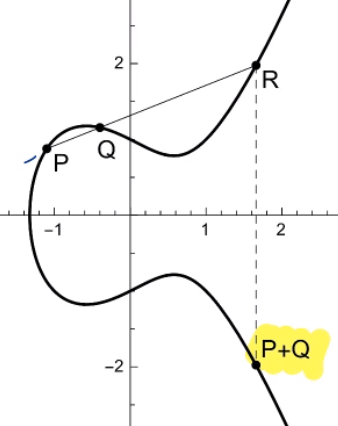
\includegraphics[scale=0.5]{15.png}\\
	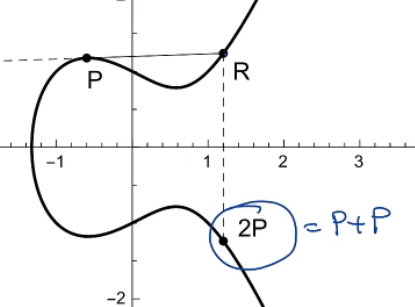
\includegraphics[scale=0.5]{16.png}
\end{center}
\end{multicols}

\paragraph{Formulazione algebrica} $P ( x_p, y_p)$, $Q = (x_q, y_q)$, $S = P + Q$\\
\begin{list}{}{}
	\item[$Q \neq \pm P$] $S = (x_s, y_s)$ con $\left\{\begin{array}{l}
	x_s = \lambda^2 - x_p - x_q\\
	y_s = -y_p + \lambda(x_p - x_s)\\
	\lambda = \frac{y_q - y_p}{x_q - x_p}
	\end{array}\right.$
	\item[$Q = P$] Stesse formule, ma $\lambda = \frac{3x_p^2 + a}{2y_p}$. Se $y_p = 0$ allora $P + P = O$
	\item[$Q = -P$] $P + Q = O$
\end{list}
\subsection{Curve Ellittiche su campi finiti}
\paragraph{Due famiglie}
\begin{list}{}{}
	\item \textbf{Curve Prime} $K = Z_p$ con $p$ primo\\
	Hanno caratteristica $p$, e sono quelle che considereremo. Imporremo $p > 3$
	\item \textbf{Curve Binarie} $K = GR(2^m)$ con $m\in N$\\
	Ha caratteristica pari a 2, quindi non si può usare la forma di Weierstrass
\end{list}
$$E_p(a, b) = \{(x,y)\in Z_p^2\:|\: y^2\textsl{ mod }p = x^3 + ax + b\textsl{ mod }p \cup \{O\}$$
Quindi in $[0, p-1]$ e ho simmetria\ldots %TODO
\begin{center}
	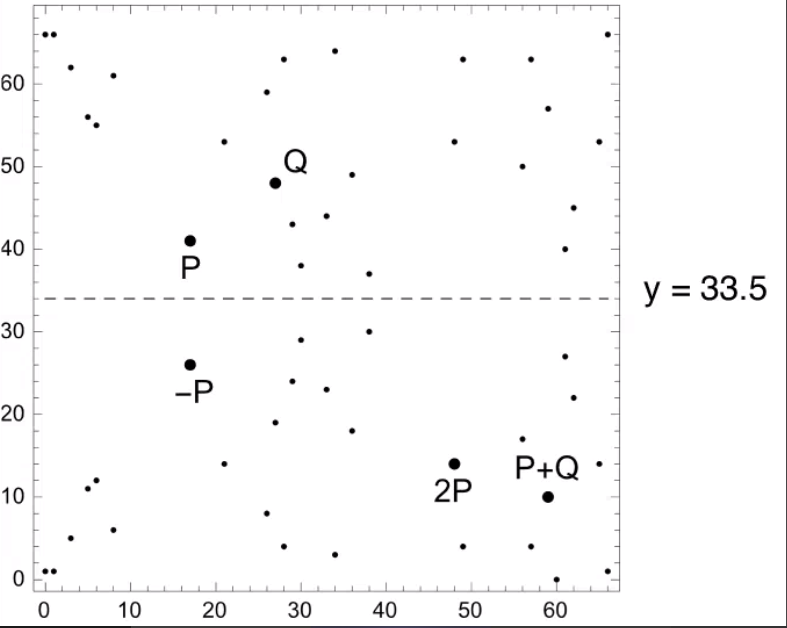
\includegraphics[scale=0.5]{17.png}\\
	$p = 67, a = -1, b = 1$
\end{center}
$P = (x,y) \in E_p(a,b) \Rightarrow -P = (x, p-y) \in E_p(a,b)$
\paragraph{Ordine} \# punti della curva. Non c'è una formula, dipende da com'è fatta la cubica $y^2 = x^3 + ax + b$ con $x \in Z_p$, quindi $p$ valori per $x$. Ogni valore possibile di $x$ da origine a 2 punti ($y$ e $-y$ per il punto opposto).\\ Ci si aspettano quindi circa $2p$ punti per i valori di $x$, +1 per $\{O\}$, ma non è esattamente $2p + 1$ perché non tutti i numeri hanno una radice nel campo. $\frac{p-1}{2}$ sono residui quadratici.\\
Quindi indicativamente il numero di punti è un numero molto vicino a $p$. Il \textbf{teorema di Hasse} che dice dato $N$ = ordine di una certa curva $E_p(a,b)$, allora $|N - (p+1)|\leq 2\sqrt{p}$
\paragraph{Esempio} $y^2 \equiv x^3 + 4x + 4$ mod $5$\\
\begin{tabular}{c | c}
$y$&$y^2$\\
\hline
0&0\\
1&1\\
2&4\\
3&4\\
4&1
\end{tabular}
1 e 4 sono residui quadratici, ammettono una radice nel campo.
\begin{list}{}{}
	\item[$x= 0$] $y^2 = 4 \Rightarrow (0,2),(0,3)\in E_5(4,4)$
	\item[$x=1$] $y^2 = 4 \Rightarrow (1,2),(1,3) \in E_5(4,4)$
	\item[$x=2$] $y^2 = 0 \Rightarrow (2,0) \in E_5(4,4)$
	\item[$x=3$] $y^2 = 3 \Rightarrow$ nessuna soluzione
	\item[$x=4$] $y^2 = 4 \Rightarrow (4,2), (4,3)\in E_5(4,4)$
	\item[$\Rightarrow$] Ordine = 8, compreso $O$
\end{list}
\begin{center}
\begin{tabular}{c | c}
Algebra modulare & Corve ellittiche\\
\hline
Moltiplicazione & Somma di punti\\
Fissato K: elevamento a potenza (one-way) & \textbf{Moltiplicazione scalare} di un punto $P$ della curva per un intero $k$\\
$y^k = y\cdot y \cdot \ldots \cdot y$, $k$ volte&$kP = P + P + \ldots + P$, $k$ volte\\
Costo polinomiale & Costo polinomiale
\end{tabular}
\end{center}
$Q = kP$ in tempo polinomiale con il metodo dei \textbf{raddoppi ripetuti}. Il problema inverso, trovare $k$ da $Q$ e $P$ è il logaritmo discreto sulle curve ellittiche, difficile.
\pagebreak
\subsection{Funzione one-way}
\paragraph{Moltiplicazione scalare} Verifichiamo che è one-way:
\begin{list}{}{}
	\item $Q = kP$ dati $k$ e $P$ è facile, con $\Theta(\log k)$ operazioni: \textbf{raddoppi ripetuti}
	\begin{list}{}{}
		\item $k = \sum_{i=0}^t k_i\cdot2^i$ con $(k_t k_{t-1}\ldots k_1 k_0) = k$ e $t + 1 = \lfloor \log_2 k\rfloor + 1$ \# bit
		\item Si calcolano i punti $2P, 4P,\ldots, 2^t P$, ciascuno come raddoppio del punto precedente: $t = \Theta(\log k)$ raddoppi
		\item Si calcola $Q = \sum_{i\:|\:k_i = 1} (2^i P)$, $O(t) = O(\log k)$ somme
	\end{list}
	Avendo un algoritmo polinomiale.
\end{list}
L'\textbf{operazione inversa} della moltiplicazione scalare: dati $P,Q\in E_p(a,b)$ trovare il più piccolo $k\:|\: Q = kP$ $$k = \log_p Q$$
È il \textbf{problema del logaritmo discreto per le curve ellittiche}, difficile per cui non conosciamo algoritmi polinomiali e nemmeno subesponenziali, soltanto forza bruta.
\subsection{Protocollo DH su curve ellittiche}
\paragraph{Preparazione} Alice e Bob scelgono una curva ellittica appropriata e un punto $B$ della curva di ordine molto grande.\\ (L'\textbf{ordine $n$ di un punto B} è \textbf{il più piccolo intero $n\:|\:nB = O$})\\
Il punto B gioca un po' il ruolo del generatore $g$ del DH standard. Curva e punto B sono \textbf{pubblici}.
\begin{center}
	\begin{tabular}{c | c | c}
	Alice & \textit{Canale} & Bob\\
	\hline
	& \makecell{$E_p(a,b)$ e $B\in E_p(a,b)$\\pubblici con B di ordine $n$} & \\
	\makecell{\textbf{Estrae}\\$n_A < n$ casuale\\\textbf{chiave privata}} & & \makecell{\textbf{Estrae}\\$n_B < n$ casuale\\\textbf{chiave privata}}\\
	& &\\
	\makecell{\textbf{Calcola} la \textbf{chiave pubblica}\\$P_A = n_A\cdot B$\\}& &\makecell{\textbf{Calcola} la \textbf{chiave pubblica}\\$P_B = n_B\cdot B$\\}\\
	& In chiaro & \\
	& $\rightarrow P_A\rightarrow$ & \\
	& $\leftarrow P_B\leftarrow$ & \\
	\textbf{Riceve} $P_B$ & & \textbf{Riceve} $P_A$\\
	& &\\
	\makecell{\textbf{Calcola}\\$S = n_A\cdot P_B = n_A\cdot n_B\cdot B$\\\texttt{k[sessione]} = $x_S$ mod $2^{256}$} & & \makecell{\textbf{Calcola}\\$S = n_B\cdot P_B = n_B\cdot n_A\cdot B$\\\texttt{k[sessione]} = $x_S$ mod $2^{256}$}
	\end{tabular}
\end{center}
\paragraph{Crittoanalista} Eve conosce la curva, il punto $B$ e intercetta $P_A$ e $P_B$ ma per calcolare $S$ deve trovare uno tra
\begin{list}{}{}
	\item $n_A\:|\:n_A\cdot B = P_A$
	\item $n_B\:|\:n_B\cdot B = P_B$
\end{list}
quindi deve \textbf{risolvere il problema del logaritmo discreto su curve ellittiche}.\\
Il protocollo è però soggetto ad attacchi attivi MitM.
\section{Scambio di messaggi cifrati}
\paragraph{Scambio di messaggi} Si trasforma il messaggio $m$ in $P_m$ punto di una curva ellittica prima $E_p(a,b)$\\
$y^2 \equiv x^3 + ax + b$ mod $p$, e possiamo pensare di sostituire $m$ a $x$, il problema è che il risultato potrebbe non essere un residuo quadratico. $P(m^3+am+b$ sia un residuo quadratico$) \simeq \frac{1}{2}$\\
\textbf{Residuo quadratico}: ha radice nel campo.\\
Tecnica con possibilità di successo così bassa non va bene, serve una tecnica migliore. Ci sono algoritmi randomizzati, \textbf{non sono noti algoritmi deterministici polinomiali}.
\subsection{Algoritmo di Koblitz}
Algoritmo polinomiale randomizzato che $m<p \mapsto P_m\in E_p(a,b)$\\
Si sceglie $h$ intero $|\:(m+1)h < p$\\
$x = m\cdot h + i$ con $0\leq i < h$ $\Rightarrow h$ tentativi per inserire $m\cdot h + i$ come ascissa e vedere se è residuo quadratico o meno.
\begin{lstlisting}
KOBLITZ(m,h,a,b,p){
	for(i = 0; i < h; i++){
		x = mh + i;
		z = (x^3 + ax + b) mod p;
		if (z residuo quadratico) { //Costo polinomiale
			y = sqrt(z);
			return Pm = (x,y);
		}
	}
	return "failure";
}
\end{lstlisting}
Probabilità di fallimento $\simeq\left(\frac{1}{2}\right)^h \Rightarrow$ probabilità di successo $\simeq 1 - \left(\frac{1}{2}\right)^h$\\
Per risalire a $m$ da $x$, $\lfloor\frac{x}{h}\rfloor = \lfloor \frac{mh + i}{h}\rfloor = \lfloor m + \frac{i}{h}\rfloor = m$ perché $\frac{i}{h} < 1$
\subsection{Scambio di messaggi} Viene fissata la curva $E_p(a,b)$ e il punto $B$ di ordine elevato $n$, $B\in E_p(a,b)$\\
Ogni utente genera \texttt{k[pub]}, \texttt{k[priv]}\begin{list}{}{}
	\item \texttt{k[priv]} è $n_u < n$
	\item \texttt{k[pub]} è $P_u$ = $n_u B$
\end{list}
Alice mittente vuole mandare un messaggio a Bob destinatario:
\begin{list}{}{}
	\item Alice converte $m$ messaggio in $P_m\in E_p(a,b)$, ad esempio con l'algoritmo di Koblitz\\
	Sceglie un intero casuale $r$ e calcola $V = rB$ ($V$ è quindi un punto a caso sulla curva $E_p(a,b)$)\\
	Calcola $W = P_m + rP_{Bob}$ e dato che $r$ è casuale, $rP_{Bob}$ è scelto a caso su $E_p(a,b)$ ($P_{Bob}$ è la chiave pubblica di Bob)\\
	Invia a Bob $\langle V,W\rangle$
	\item Bob riceve $\langle V,W\rangle$\\
	Decifra $W - n_{Bob}V = (P_m + rP_{Bob}) - n_{Bob}V = P_m + rn_{Bob}B - n_{Bob}rB = P_m$\\
	Ricava $m = \lfloor \frac{x}{h}\rfloor$\\
\end{list}
La sicurezza è basata sulla difficoltà del logaritmo discreto su curve ellittiche.
\paragraph{Crittoanalista} Potrebbe decifrare in questi modi, dallo stesso costo:
\begin{list}{}{}
	\item Se trova $r$, decifra facendo $W - rP_{Bob} = (P_m +rP_{Bob}) - rP_{Bob}$\\
	Ma per trovare $r$ da $V,B$, $V = rB$ bisogna risolvere il logaritmo discreto\\
	Consente di decifrare un solo crittogramma ($r$ è one time).
	\item Altrimenti deve trovare $n_{Bob}$ da $P_{Bob},B$\\
	$P_{Bob} = n_{Bob}B$, logaritmo discreto\\
	Consentirebbe di decifrare tutti i crittogrammi successivi.
\end{list}
\paragraph{Sicurezza} Per attaccare RSA, DH, El Gamal (algebra modulare) $O(2^{\sqrt{b\cdot\log b}})$, con $b$ = \# bit del modulo (basati su \textbf{index calculus}, sfruttano la proprietà algebrica dei campi $Z_p$)\\
Per attaccare su curve ellittiche (logaritmo discreto su curva ellittica) $O(2^{\frac{b}{2}})$, con $b$ \# bit dell'ordine di B
\chapter{Identificazione, Autenticazione e Firma Digitale}
\paragraph{Identificazione} Un sistema di elaborazione, isolato o in rete, deve \textbf{essere in grado di accertare l'identità di un utente} che richiede di accedere ai suoi servizi.
\paragraph{Autenticazione} Il destinatario di un messaggio deve \textbf{essere in grado di accertare l'identità del mittente e l'integrità del crittogramma ricevuto}
\paragraph{Firma Digitale} \begin{enumerate}
	\item Il \textbf{mittente non deve poter negare di aver inviato} un messaggio $m$
	\item Il \textbf{destinatario deve essere in grado di autenticare} il messaggio
	\item Il \textbf{destinatario non deve poter sostenere che} $m'\neq m$ è il messaggio inviato dal mittente
\end{enumerate}
Tutto deve essere verificabile da una terza parte.
\paragraph{Relazioni tra le funzionalità} Non sono indipendenti, ma \textbf{ciascuna estende le precedenti}:
\begin{list}{}{}
	\item L'autenticazione di un messaggio garantisce l'identificazione del mittente
	\item L'apposizione della firma garantisce l'autenticazione del messaggio
\end{list}
Ogni funzionalità e utilizzata per contrastare gli attacchi attivi. Esistono \textbf{realizzazioni algoritmiche basate su cifrari asimmetrici e simmetrici}.
\section{Funzioni hash} Funzione hash è una funzione $f:X\rightarrow Y$ tale che $n = |X| >> m = |Y|$\\
$\exists\:X_1,X_2,\ldots,X_m \subseteq X$ disgiunti tali che $X = X_1 \cup X_2 \cup \ldots \cup X_m\wedge\forall\:i,\forall\:x\in X_i$ ho $f(x) = y$\\
Comodo per gestire la rappresentazione compatta dei dati.\\\\
Una \textbf{buona funzione hash} assicura che:
\begin{list}{}{}
	\item I sottoinsiemi $X_1,\ldots,X_m$ hanno circa la stessa cardinalità.\\
	Due elementi estratti a caso da $X$ hanno probabilità circa $\frac{1}{m}$ di avere la stessa immagine in $Y$
	\item Elementi di $X$ molto "simili" tra loro appartengono a due sottoinsiemi diversi.\\
	Ad esempio se $X$ è un insieme di interi, due elementi con valori prossimi devono avere immagini diverse.
	\item Gestione delle collisioni.\\
	L'algoritmo che impiega la funzione hash dovrà affrontare la situazione in cui più elementi di $X$ hanno la stessa immagine in $Y$
\end{list}
\subsection{Funzioni hash one-way} Se la funzione è usata in crittografia, deve \textbf{soddisfare le seguenti proprietà}:
\begin{enumerate}
	\item $\forall\:x\in X$ è \textbf{computazionalmente facile} calcolare $y = f(x)$\\
	(Ricordiamo che computazionalmente facile significa tempo polinomiale nella dimensione di $x$)
	\item \textbf{Proprietà one-way}: per la maggior parte degli $y\in Y$ è \textbf{computazionalmente difficile} determinare\\$x\in X\:|\:f(x) = y$ cioè $x = f^{-1}(y)$\\
	(Ricordiamo che computazionalmente difficile significa tempo esponenziale)
	\item \textbf{Proprietà claw-free}: è \textbf{computazionalmente difficile} determinare $x_1,x_2\:|\:f(x_1) = f(x_2)$, cioè due elementi diversi che collidono sulla stessa immagine hash.
\end{enumerate}
\paragraph{Funzioni hash usate in crittografia}
\begin{list}{}{}
	\item \textbf{MD5} Message Digest, versione 5\\
	Famiglia di algoritmi, vennero pubblicati MD2 e MD4 ma avevano debolezze. MD5 proposto da Ron Rivest nel 1992.\\
	Input: sequenza $S$ di 512 bit\\
	Output: \textbf{immagine di 128 bit}. La sequenza è \textit{digerita}, riducendone la lunghezza ad un quarto.\\
	Dal 2004 è considerato severamente compromesso, poiché è stato dimostrato che non resiste alle collisioni ed ha altre debolezze serie.
	\item \textbf{RIPEMD-160}\\
	Versione "matura" delle funzioni MD. Produce immagini di 160 bit ed è esente dai difetti di MD5.
	\item \textbf{SHA} Secure Hash Algorithm\\
	Viene adottato quando la proprietà claw-free è cruciale per la sicurezza del sistema.\\
	Opera su sequenze lunghe fino a $2^{64}$ bit e produce immagini di 160 bit.\\
	\textbf{Crittograficamente sicura}: soddisfa i requisiti delle funzioni hash one-wat e genere immagini molto diverse per sequenze molto simili.
	\begin{list}{}{}
		\item \textbf{SHA-1}, opera su sequenze fino a $2^{64}-1$ bit e produce immagini di 160 bit. Molto usato nei protocolli crittografici anche se non è più certificato come standard. Tutte le altre funzioni hanno una struttura simile a SHA-1.\\
		Opera su blocchi da 160 bit, contenuti un buffer da 5 registri di 32 bit ciascuno, in cui sono caricati inizialmente dei valori pubblici. Il messaggio $m$ viene concatenato con una sequenza di padding che ne rende la lunghezza multipla di 512 bit. Il contenuto dei registri varia nel corso dei cicli successivi, in cui questi valori si combinano tra loro e con blocchi di 32 bit provenienti da $m$.\\
		A fine procedimento, i registri contengono SHA-1($m$)
		\begin{multicols}{2}
			\begin{center}
				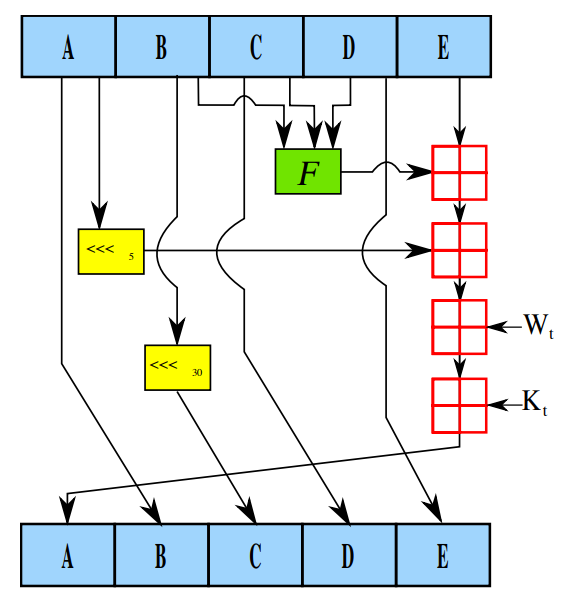
\includegraphics[scale=0.5]{18.png}Z
			\end{center}
				Un'iterazione all'interno di SHA-1.\\
				A,B,C,D,E sono i registri a 32 bit.\\
				F è una funzione non lineare che varia.\\
				$<<<_n$ denota una rotazione del bit di sinistra di $n$ posti.\\
			$n$ varia per ogni operazione.\\
			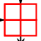
\includegraphics[scale=0.33]{19.png} denota l'addizione in modulo $2^{32}$\\
			$K_t$ è una costante\\
			$W_t$ blocco di 32 bit ottenuto tagliando e rimescolando i blocchi del messaggio\\\\
			Il contenuto dei registri, che partono con valori pubblici, varia nel corso dei cicli combinandosi tra loro e con blocchi da 32 bit provenienti dal messaggio $W$, nonché con alcuni parametri relativi al ciclo.\\
			Alla fine del procedimento, quando è stato letto l'intero messaggio, i registri conterranno SHA-1($W$)
		\end{multicols}
	\end{list}
\end{list}
\section{Identificazione su canali sicuri}
\paragraph{Esempio} L'accesso di un utente alla propria casella di posta elettronica, o a file personali memorizzati su un sistema con accesso riservato ai membri della sua organizzazione.\\L'utente inizia il collegamento inviando in chiaro login e password. Se il canale è protetto in lettura e scrittura, un attacco può essere sferrato solo da un utente locale al sistema: ad esempio l'amministratore che ha accesso a tutti i file memorizzati (o un hacker).
Il meccanismo di identificazione prevede una \textbf{cifratura delle password realizzata con funzioni hash one-way}.

\subsection{Cifratura delle password nei sistemi UNIX}
Quando un utente $U$ fornisce per la prima volta la propria password $P$, il \textbf{sistema associa ad $U$ due sequenze binarie} che memorizza nel file delle password al posto di $P$:
\begin{list}{}{}
	\item $S$, seme, prodotta da un generatore pseudocasuale
	\item $Q = h(PS)$ con $h$ funzione hash one-way e $PS$ concatenazione semplice della password e del seme.
\end{list}
Per proteggere da attacchi interni è quindi necessario hashare le password: il seme è utile per non hashare password uguali di utenti diversi con stesso hash.\\\\
Ad ogni successiva connessione di $U$, il sistema:
\begin{list}{}{}
	\item Recupera $S$ dal file delle password
	\item Concatena $S$ con la password fornita da $U$
	\item Calcola l'immagine one-way della nuova sequenza: $h(PS)$
	\item Se $h(PS) = Q$, l'identificazione ha successo.
\end{list}
Un accesso illecito al file delle password, quindi, non fornisce informazioni interessanti: è \textbf{computazionalmente difficile ricavare la password originale dalla sua immagine one-way}.
\subsection{Protezione del canale}
Se il canale è insicuro, la password può essere intercettata durante la trasmissione in chiaro. Il \textbf{sistema non dovrebbe mai maneggiare direttamente la password, ma una sua immagine inattaccabile}.
\paragraph{Canale insicuro: identificazione} $\langle e,n\rangle,\langle d\rangle$: chiave pubblica e privata di un utente $U$ che richiede l'accesso ai servizi offerti dal sistema $S$
\begin{enumerate}
	\item $S$ genera un numero casuale $r < n$ e lo invia in chiaro a $U$
	\item $U$ calcola $f = r^d$ mod $n$, \textbf{firma di $U$ su $r$}, con la sua chiave privata e lo spedisce ad $S$
	\item $S$ verifica la correttezza del valore ricevuto calcolando e verificando se $f^e$ mod $n = r$\\
	Se ciò avviene, l'identificazione ha successo.
\end{enumerate}
Le operazioni di cifratura e decifrazione sono invertite rispetto all'impiego standard dell'RSA, ma questo è possibile perché le due operazioni sono commutative:
$$(x^e\textsl{ mod }n)^d\textsl{ mod }n = (x^d\textsl{ mod }n)^e\textsl{ mod }n = x$$
$f$ può essere generata solo da $U$ che possiede $\langle d\rangle$. Se il passo 3 va a buon fine, il sistema ha la garanzia che l'utente che ha richiesto l'identificazione sia effettivamente $U$, anche se il canale è insicuro.
\textbf{Problema}: $S$ chiede ad $U$ di applicare la chiave privata ad una sequenza $r$ che $S$ stesso ha generato, potrebbe essere stata \textbf{scelta di proposito per ricavare qualche informazioni sulla chiave privata di $U$}\\
\textbf{Protocollo alternativo}, a "\textbf{conoscenza zero}": impedisce che da una comunicazione si possa estrarre più di quanto sia nelle intenzioni del comunicatore.
\pagebreak
\paragraph{Canale insicuro: autenticazione} DEST deve \textbf{autenticare il messaggio}, accertando l'identità di MITT e l'integrità di $m$. MITT e DEST concordano una chiave segreta $k$.\\
MITT:
\begin{list}{}{}
	\item Allega al messaggio un \textbf{MAC} (Message Authentication Code) $A(m,k)$, allo scopo di garantire la provenienza e l'integrità del messaggio.
	\item Spedisce la coppia $\langle m, A(m,k)\rangle$ in chiaro\\
Oppure cifra $m$ e spedisce $\langle C(m,k'), A(m,k)\rangle$ con $C$ funzione di cifratura e $k'$ chiave pubblica o segreta del cifrario scelto.
\end{list}
DEST:
\begin{list}{}{}
	\item Entra in possesso di $m$, eventualmente dopo averlo decifrato
	\item Essendo a conoscenza di $A$ e $k$, calcola $A(m,k)$
	\item Confronta il valore ottenuto con quello ricevuto da MITT per verificare che il MAC ricevuto corrisponda al messaggio a cui risulta allegato.\\
	Se la verifica ha successso, il messaggio è autenticato. Altrimenti, DEST scarta il messaggio.
\end{list}
Il \textbf{MAC} è un'immagine breve del messaggio, che può essere stata generata solo da un mittente conosciuto dal destinatario, previ opportuni accordi.\\
Ci sono varie proposte, basate su cifrari asimmetrici, simmetrici e funzioni hash one-way.
\subparagraph{MAC con funzioni hash one-way} $A(m,k) = h(mk)$ con $h$ funzione hash one-way.\\
Risulta computazionalmente difficile per un crittoanalista scoprire la chiave segreta $k$. $h$ è nota a tutti e $m$ può viaggiare in chiaro o essere scoperto per altra via, ma $k$ viaggia all'interno del MAC. Per recuperare $k$ bisognerebbe invertire $h$.\\
Il crittoanalista non può sostituire facilmente $m$ con un altro messaggio $m'$, dovrebbe allegare alla comunicazione di $m'$ il MAC $A(m',k) = h(m'k)$ che può produrre solo conoscendo $k$.
\subparagraph{CBC+MAC} Usando un cifrario a blocchi in modalità CBC (Cipher Block Chaining), si può usare il blocco finale del crittogramma come MAC. Il blocco finale, infatti, è funzione dell'intero messaggio.
\subsection{Firma digitale}
Una firma manuale ha i seguenti \textbf{requisiti}:
\begin{enumerate}
	\item \textbf{Autentica e non falsificabile}\\
	Prova che chi l'ha prodotta è chi ha sottoscritto il documento
	\item \textbf{Non è riutilizzabile}\\
	Legata strettamente al documento su cui è stata apposta
	\item \textbf{Il documento firmato non è alterabile}\\
	Chi ha prodotto la firma è sicuro che questa si riferirà solo al documento sottoscritto nella sua forma originale
	\item \textbf{Non può essere ripudiata da chi l'ha apposta}\\
	Costituisce prova legale di un accordo o dichiarazione
\end{enumerate}
La \textbf{firma digitale} non può consistere semplicemente nella digitalizzazione del documento originale firmato manualmente. Un crittoanalista potrebbe "tagliare" dal documento digitale la parte contenente la firma e "copiarla" su un altro documento.\\
Deve avere una forma dipendente dal documento su cui è apposta, per essere inscindibile da questo. Per progettare firma digitali si possono usare sia cifrari simmetrici che asimmetrici.
\paragraph{Protocollo 1} Messaggio $m$ in chiaro e firmato.
\begin{list}{}{}
	\item $U$ utente, \texttt{k$_U$[priv]} e \texttt{k$_U$[pub]} chiavi di $U$
	\item $C,D$ funzioni di cifratura e decifrazione di un cifrario asimmetrico
	\item \textbf{Firma} U genera la firma $f = D(m,$ \texttt{k$_U$[priv]}$)$ per $m$ e spedisce all'utente $V$ la tripla $\langle U,m,f\rangle$
	\pagebreak
	\item \textbf{Verifica} V riceve $\langle U,m,f\rangle$ e verifica l'autenticità della firma $f$ controllando che $C(f,$ \texttt{k$_U$[priv]}$) = m$\\
	L'indicazione del mittente $U$ consente a $V$ di selezionare la chiave pubblica \texttt{k$_U$[pub]} da utilizzare nel calcolo.\\
I processi di firma e verifica impiegano le funzioni $C,D$ in ordine inverso a quello standard, quindi devono essere commutative $C(D(m)) = D(C(m)) = m$	
\end{list}
Posso sostituire $m$ con $c$ crittogramma? La verifica richiede la conoscenza della chiave pubblica e restituisce $m$, quindi non avrebbe senso sostituire $m$ con $c$.\\
Il protocollo soddisfa i requisiti della firma manuale:
\begin{list}{}{}
	\item $f$ è autentica e non falsificabile (1)\\
	\texttt{k$_U$[priv]} è nota solo a $U$ e per falsificare la firma occorre conoscere \texttt{k$_U$[priv]} ma $D$ è one-way
	\item Il documento firmato $\langle U,m,f\rangle$ non può essere alterato se non da $U$, pena la non consistenza fra $m$ e $f$ (3)
	\item Poiché solo $U$ può aver prodotto $f$, $U$ non può ripudiare la firma (4)
	\item La firma $f$ non è riutilizzabile su un altro documento $m'\neq m$ poiché è immagine di $m$ (2)
\end{list}
Definito per un particolare utente $U$ ma non per un particolare destinatario, quindi \textbf{chiunque può convincersi dell'autenticità della firma} facendo uso solo della chiave pubblica di $U$. Si tratta di uno \textbf{schema di principio}: comporta lo scambio di un messaggio di lunghezza doppia dell'originale, poiché la dimensione della firma è paragonabile alla dimensione del messaggio, ed \textbf{il messaggio non può essere cifrato} perché è \textbf{ricavabile pubblicamente} dalla firma attraverso la verifica di questa.
\paragraph{Protocollo 2} Messaggio $m$ cifrato e firmato.\\
\textbf{Firma e cifratura}:
\begin{list}{}{}
	\item $U$ genera la firma $f = D(m,$ \texttt{k$_U$[priv]}$)$ per $m$, calcola il crittogramma firmato $c = C(f,$ \texttt{k$_V$[pub]}$)$ con la chiave pubblica del destinatario $V\rightarrow$ si incapsula la firma nel documento cifrato.
	\item Spedisce $\langle U,c\rangle$ a $V$
\end{list}
\textbf{Decifrazione e verifica}:
\begin{list}{}{}
	\item $V$ riceve $\langle U,c\rangle$ e decifra il crittogramma $D(c,$ \texttt{k$_V$[priv]}$) = f$
	\item Cifra tale valore con la chiave pubblica di $U$ ottenendo $C(f,$ \texttt{k$_U$[pub]}$) = C(D(m,$ \texttt{k$_U$[priv]}$),$ \texttt{k$_U$[pub]}$) = m$
	\item $V$ ricostruisce $m$ e se è significativo attesta l'identità di $U$\\
	Un utente diverso da $U$ ha probabilità praticamente nulla di generare un crittogramma di significato accettabile se cifrato con la chiave pubblica di $U$
\end{list}
\subparagraph{Algoritmo} Cifrario RSA con\begin{list}{}{}
	\item $\langle d_U\rangle,\langle e_U, n_U\rangle$ chiavi di $U$
	\item $\langle d_V\rangle,\langle e_V, n_V\rangle$ chiavi di $V$
\end{list}
Utente $U$\begin{list}{}{}
	\item Genera la firma del messaggio $m$: $f = m^{d_U}$ mod $n_U$
	\item Cifra $f$ con la chiave pubblica di $V$: $c = f^{e_V}$ mod $n_V$
	\item Spedisce a $V$ $\langle U,c\rangle$

\end{list}
Utente $V$\begin{list}{}{}
	\item Riceve $\langle U,c\rangle$ e decifra $c$: $c^{d_V}$ mod $n_V = f$
	\item Decifra $f$ con la chiave pubblica di $U$: $F^{e_U}$ mod $n_U = m$
	\item Se $m$ è significativo, conclude che è autentico
\end{list}
Perché sia corretto, è necessario che $n_U\leq n_V$ perché risulti $f< n_V$ e $f$ possa essere cifrata correttamente e spedita a $V$. Questo impedirebbe a $V$ di inviare messaggi firmati e cifrati a $U$.\\
Ogni utente stabilisce chiavi distinte per la firma e la cifratura. Si fissa pubblicamente $H$ molto grande, es $H = 2^{1024}$, e le chiavi di firma $ < H$ mentre quelle di cifratura $> H$.\\
Questo valore alto assicura di scegliere chiavi sufficientemente grandi. Il meccanismo di firma si presta però a diversi attacchi, basati sulla possibilità del crittoanalista di procurarsi la firma di un utente su messaggi apparentemente privi di senso.
\pagebreak
\subparagraph{Attacco 1} Supponiamo che un utente $U$ invii una risposta automatica (ACK) a MITT ogni volta che riceve un messaggio $m$. Poniamo che l'ACK sia il crittogramma della firma di $U$ su $m$.\\
Un crittoanalista attivo $X$ può decifrare i messaggi inviati a $U$:
\begin{list}{}{}
	\item $X$ intercetta il crittogramma $c$ firmato inviato da $V$ a $U$, lo rimuove dal canale e lo rispedisce a $U$, facendogli credere che $c$ sia stato inviato da lui.
	\item $U$ spedisce automaticamente a $X$ un ACK
	\item $X$ usa l'ACK per risalire al messaggio originale $m$ applicando le funzioni del cifrario con le chiavi pubbliche di $V$ e $U$
\end{list}
\begin{enumerate}
	\item $V$ invia il crittogramma $c$ a $U$\\
	$c = C(f, k_U[pub])$\\
	$f = D(m, k_V[priv])$
	\item Il crittoanalista $X$ intercetta $c$, lo rimuove dal canale e lo rispedisce a $U$ ($U$ crede che $c$ arrivi da $X$)
	\item $U$ decifra $c$\\
	$f = D(c, k_U[priv])$\\
	e verifica la firma con la chiave pubblica di $X$ ottenendo il messaggio\\
	$m' = C(f, k_X[pub])$
	\item $m'\neq m$ è un messaggio privo di senso, ma il sistema manda ACK $c'$ a $X$\\
	$f' = D(m', k_U[priv])$\\
	$c' = C(f', k_X[pub])$
	\item $X$ usa $c'$ per risalire a $m$
	\begin{enumerate}
		\item Decifra $c'$ e trova $f'$\\
		$D(c',k_X[priv])=D(C(f',k_X[pub]), k_X[priv]) = f'$
		\item Verifica $f'$ e trova $m'$\\
		$C(f',k_U[pub]) = C(D(m',k_U[priv]),k_U[pub]) = m'$
		\item Da $m'$ ricava $f$\\
		$D(m',k_X[priv]) = D(C(f,k_X[pub]), k_X[priv]) = f$
		\item Verifica $f$ con la chiave pubblica di $V$ e trova $m$\\
		$C(f,k_V[pub]) = C(D(m,k_V[priv]),k_V[pub]) = m$	
	\end{enumerate}
\end{enumerate}
Per evitare questo tipo di attacco, $U$ deve bloccare l'ACK automatico che deve essere inviato solo dopo un esame preventivo di $m$ e scartando i messaggi che non si desidera firmare.\\\\
\textbf{Protocollo resistente agli attacchi}: si \textbf{evita la firma diretta del messaggio}, si appone la firma digitale su una immagine del messaggio ottenuta con una funzione hash one-way e pubblica (MD5, SHA\ldots).\\
Non si firma il messaggio ma l'hash del messaggio, il che \textbf{rompe tutti i giochi algebrici} che potevano essere eseguiti.
\paragraph{Protocollo 3} Messaggio $m$ cifrato e firmato in hash.\\
\textbf{Firma e cifratura}\begin{list}{}{}
	\item Il mittente $U$ calcola $h(m)$ e genera la firma $f = D(h(m), k_u[priv])$
	\item Calcola separatamente il crittogramma $c = C(m, k_V[pub])$
	\item Spedisce a $V$ la tripla $\langle U,c,f\rangle$
\end{list}
\textbf{Decifrazione e verifica}\begin{list}{}{}
	\item $V$ riceve $\langle U,c,f\rangle$
	\item Decifra il crittogramma $c$: $m = D(c, k_V[priv])$
	\item Calcola separatamente $h(m)$ e $C(f,k_U[pub])$
	\item Se $h(m) = C(f, k_U[pub])$, allora conclude che il messaggio è autentico.
\end{list}
Si scambiano una maggiore quantità di dati, ma l'incremento è trascurabile. La firma può essere calcolata più velocemente.
\pagebreak
\section{Attacchi man-in-the-middle}
\paragraph{Debolezza dei protocolli} Le chiavi di cifratura sono pubbliche e non richiedono un incontro diretto tra gli utenti per il loro scambio.\\
Un crittoanalista attivo può intromettersi proprio in questa fase iniziale del protocollo, pregiudicando il suo corretto svolgimento. Un attacco attivo chiamato \textbf{man-in-the-middle}:
\begin{list}{}{}
	\item Il crittoanalista si intromette nella comunicazione tra $U$ e $V$
	\item Si comporta come $V$ agli occhi di $U$
	\item Si comporta come $U$ agli occhi di $V$
	\item Intercetta e blocca le comunicazioni tra $U$ e $V$
\end{list}
\paragraph{Attacchi MitM sulle chiavi pubbliche} Il crittoanalista $X$ devia le comunicazioni che provengono da $U$ e $V$ e le dirige verso sé stesso:
\begin{list}{}{}
	\item $U$ richiede a $V$ la chiave pubblica (tramite mail, pagina web\ldots)
	\item $X$ intercetta la risposta che contiene \texttt{k$_V$[pub]} e la sostituisce con la sua chiave pubblica \texttt{k$_X$[pub]}
	\item $X$ si pone in ascolto dei crittogrammi spediti da $U$ a $V$, cifrati mediante \texttt{k$_X$[pub]}
	\item $X$ rimuove dal canale ciascuno di questi crittogrammi, li decritta, li cifra mediante \texttt{k$_V$[pub]} e li rispedisce a $V$
	\item $U$ e $V$ non si accorgeranno della presenza di $X$ se il processo di intercettazione e rispedizione è sufficientemente veloce da rendere il relativo ritardo apparentemente attribuibile alla rete.
\end{list}
\section{Certification Authority}
Un algoritmo crittografico è tanto robusto quanto la sicurezza delle sue chiavi. Lo scambio/generazione della chiave è un passo cruciale. Gli attacchi MitM sono i principali problemi di sicurezza da affrontare.\\
Sono così nate le certification authority: sono \textbf{infrastrutture che garantiscono la validità delle chiavi pubbliche} e ne regolano l'uso, \textbf{gestendo la distribuzione} sicura delle chiavi delle due entità che vogliono comunicare.
\paragraph{Key Certification Authority (CA)} Ente preposto alla certificaizone di validità delle chiavi pubbliche.\\
La CA autentica l'associazione $\langle$utente, chiave pubblica$\rangle$ emettendo un \textbf{certificato digitale}, che \textbf{consiste della chiave pubblica e di una lista di informazioni relative al proprietario}, opportunamente firmate dalla CA.\\
Per svolgere correttamente il suo ruolo, la CA mantiene un archivio di chiavi pubbliche sicuro, accessibile a tutti e protetto da attacchi in scrittura non autorizzati.\\
La chiave pubblica della CA è nota a tutti gli utenti, che la mantengono protetta da attacchi esterni e la utilizzano per verificare la firma della CA stessa sui certificati.
\paragraph{Certificato digitale} Un certificato digitale contiene:
\begin{list}{}{}
\item una indicazione del suo formato (numero di versione)
\item il nome della CA che lo ha rilasciato
\item un numero seriale che lo individua univocamente all'interno della CA emittente
\item la specifica dell'algoritmo usato dalla CA per creare la firma elettronica
\item il periodo di validità del certificato (data di inizio e data di fine)
\item il nome dell'utente a cui questo certificato si riferisce e una serie di informazioni a lui legate
\item un'indicazione del protocollo a chiave pubblica adottato da questo utente
per la cifratura e la firma: nome dell'algoritmo, suoi parametri, e chiave pubblica dell'utente
\item firma della CA eseguita su tutte le informazioni precedenti
\end{list}
\pagebreak
\paragraph{CA} Se $U$ vuole comunicare con $V$, richiede \texttt{k$_V$[pub]} alla CA che risponde inviando a $U$ il certificato cert$_V$ di $V$.\\
Poiché $U$ conosce \texttt{k$_{CA}$[pub]}, può controllare l'autenticità del certificato verificandone il periodo di validità e la firma prodotto dalla CA su di esso.\\
Se tutti i controlli vanno a buon fine, \texttt{k$_V$[pub]} nel certificato è corretta e $U$ avvia la comunicazione con $V$.\\
Un crittoanalista potrebbe intromettersi solo falsificando la certificazione, ma si assume che la CA sia fidata e il suo archivio di chiavi sia inattaccabile.
\paragraph{Organizzazione} In ogni stato \textbf{esistono diverse CA organizzate ad albero}. La verifica di un certificato è in questo caso più complicata e si svolgi attraverso una catena di verifica hce vanno dalla CA di $U$ alla CA di $V$.\\
$V$ invia ad $U$ una sequenza di caratteri ordinati in accordo alla CA che li ha firmati, da quella che ha certificato $V$ a quella che è la radice dell'albero delle CA.\\\\
\textbf{Ogni utente mantiene localmente al sistema una copia del proprio certificato cert$_U$ e una copia di} \texttt{k$_{CA}$[pub]}.\\
Interagisce con la CA una sola volta, e poi la gestione delle chiavi pubbliche diventa decentralizzata.
\paragraph{Protocollo 4} Messaggio $m$ cifrato, firmato in hash e certificato.\\
\textbf{Firma, cifratura e certificazione}
\begin{list}{}{}
	\item Il mittente $U$ si procura il certificato cert$_V$ di $V$
	\item Calcola $h(m)$ e genera la firma $f = (D(h(m), k_U[priv])$
	\item Calcola il crittogramma $c = C(m, k_V[pub])$
	\item Spedisce a $V$ la tripla $\langle$ cert$_U, c,f\rangle$\\
cert$_U$ contiene $k_U[pub]$ e la specificazione della funzione $h$ usata	
\end{list}
\textbf{Verifica del certificato}
\begin{list}{}{}
	\item Il destinatario $V$ riceve $\langle$ cert$_U, c,f\rangle$ e verifica l'autenticità di cert$_U$ (e quindi di $k_U[pub]$) utilizzando la propria copia di $k_{CA}[pub]$
\end{list}
\textbf{Decifrazione e verifica della firma}
\begin{list}{}{}
	\item $V$ decifra il crittogramma $c$ con la propria chiave privata e ottiene $m = D(c, k_V[priv])$
	\item $V$ verifica l'autenticità della firma apposta da $U$ su $m$ controllando che risulti $C(f,k_U[pub]) = h(m)$
\end{list}
\paragraph{Conclusioni} Il punto debole del meccanismo delle CA è rappresentato dai certificati revocati. La CA mettono a disposizione un archivi con i certificati non più validi.\\
La \textbf{frequenza di controllo di questi certificati} e le modalità della loro comunicazione agli utenti sono \textbf{cruciali per la sicurezza}.\\
Attacchi MitM possono essere evitati se si stabilisce un incontro diretto tra un utente e la CA nel momento in cui si istanza il sistema asimmetrico dell'utente.
\section{Protocollo Zero Knowledge}
\paragraph{Protocollo a conoscenza zero} Lo vedremo all'opera per l'identificazione. Silvio Micali, premio Turing, e Shefi Goldwasser (MIT, 1989).
\paragraph{Obiettivo} Due utenti: \textbf{prover} e \textbf{verifier}, anche chiamati Peggy/Victor.\\
Il protocollo è uno scambio tra P e V, composto da una serie di sfide che P deve superare per convincere V di essere in possesso di una certa informazione. Scambio di messaggi che permette a P di \textbf{dimostrare} a V, e a fine protocollo V deve ragionevolmente convincersi che P possiede l'informazione.
\paragraph{Esempio} Peggy sostiene di poter contare i granelli di sabbia di una spiaggia solamente guardandola, e Victor vuole controllare se quanto dice Peggy è vero (\textbf{non con certezza}, ma con probabilità prossima a 1).\\
Victor sceglie la spiaggia e ci va con Peggy. \textbf{Fase di preparazione} dove Victor chiede a Peggy di comunicare la parità dei granelli di sabbia.
$$P \rightarrow^{b_0} V\:\:\:\:\:b_0 =\textsl{ parità dei granelli di sabbia}$$
\pagebreak
Dopodiché, il protcollo funziona così:
\begin{lstlisting}
	for (i=1 to k) { //k scelto da V
		P si volta;
		V sceglie un e bit (0, 1) casuale;
		if (e==0) V toglie un granello di sabbia
		V chiede a P il nuovo valore bi //chiede nuovamente parita granelli
		if ((e == 0 && b[i] != b[i-1]) || //parita cambiata perche tolto granello
			(e == 1 && b[i] == b[i-1])) //parita non cambiata
				continua alla prossima iterazione;
		else //P impostore
				STOP
	}
	//P dice il vero con probabilita 1-(1/2)^k
\end{lstlisting}
La probabilità di vincere una sfida ingannando, se Peggy è disonesta, è la probabilità di indovinare il bit generato, $\frac{1}{2}$. Quindi la probabilità di vincere ingannando è di farlo per $k$ volte, cioè $\left(\frac{1}{2}\right)^k$.\\
Quindi, la probabilità di ingannare V è $\left(\frac{1}{2}\right)^k$.\\
La probabilità che P abbia la capacità assunta è almeno $1-\left(\frac{1}{2}\right)^k$\\
\textbf{Evidenza sperimentale significativa}, ma \textbf{non dimostrazione rigorosa}, che P abbia la capacità/conoscenza.
\subsection{Proprietà di un protocollo zero knowledge}
\paragraph{Principi generali}\begin{enumerate}
	\item \textbf{Completezza}\\
	Se P è onesto (la sua affermazione è vera), V \textbf{accetta sempre} la dimostrazione. Cioè P deve sempre poter superare le sfide di V.
	\item \textbf{Correttezza}\\
	Se P è disonesto (la sua affermazione è falsa), V \textbf{può essere ingannato} con probabilità $\leq \left(\frac{1}{2}\right)^k$ con $k$ scelto da V
	\item \textbf{Conoscenza zero}\\
	Se l'affermazione di P è vera, il verificatore V (anche se disonesto) non può alcuna informazione se non la veridicità di questo fatto.
\end{enumerate}
\subsection{Protocollo di identificazione a conoscenza zero}
\paragraph{Protocollo di Fiat-Shamir} Uno dei primi nati. P dimostra a V la sua identità senza svelare alcun'altra informazione.\\
Basato sulla difficoltà di calcolo della radice quadrata in modulo $n$ composto.\\
$t = s^2$ mod $n$, $n$ composto. Victor conosce $t,n$, Peggy deve convincere $V$ di conoscere $s = \sqrt{t}$. Deve succedere in tempo polinomiale, altrimenti in tempo esponenziale V può calcolarsela.
\begin{list}{}{}
	\item \textbf{Fase di preparazione}\\
	P sceglie $p,q$ primi molto grandi e calcola $n = p\cdot q$ e sceglie $s < n$ segreto. Calcola $t = s^2$ mod $n$.\\
	Tutte attività eseguibili in tempo polinomiale.
	\item P rende nota $\langle t,n\rangle$ (chiave \textbf{pubblica}) e mantiene segreta $\langle p,q,s\rangle$ (chiave \textbf{privata})\\
	$p,q,s$ sono calcolabili in tempo polinomiale solo conoscendo $t,n$.\\
	Se P è la proprietaria della chiave privata, sarà in grado di convincere qualunque verificatore con probabilità $1-\left(\frac{1}{2}\right)^k$ senza che acquisica maggiori informazioni.
	\item \textbf{Protocollo}, ripeti $k$ volte:
	\begin{enumerate}
		\item V chiede a P di iniziare una iterazione
		\item P genera un intero $r<n$ casuale, ne calcola $u = r^2$ mod $n$ e comunica $u$ a V.
		Numero casuale usato per la sfida e buttato via.
		\item V genera il \textbf{bit casuale} $e$ e lo comunica a P
		\item P calcola $z = r\cdot s^e$ mod $n$ e comunica $z$ a V\\
Se $e = 0$, $z = r$. Se $e = 1$, $z = r\cdot s$ mod $n$
		\item V	calcola $x = z^2$ mod $n$\\
		$(rs^e)^2 = r^2(s^e)^2 = u(s^2)^e = ut^e$\\
		Se $x = ut^e$ mod $n$ allora sfida superata, si va alla successiva.\\
		Altrimenti STOP, P non è identificato.
	\end{enumerate}
	$r$ non viaggia mai in chiaro, tranne quando $e=0$ cioè $z=r$. $s$ non viaggia mai da solo, ma $r$ è legato alla sola sfida quindi non è un problema.
\end{list}
Tutte le volte che $e=0$ la sfida è facile da superare. Perché non si chiede sempre di usare $e=1$, cioè di usare il segreto? Ad esempio, V manda sempre $e=1$. P può imbrogliare e superare sempre. P si aspetta sempre $e=1$, al passo 2. sceglie $r$ a caso e invia a V non $u=r^2$ ma $u = \frac{r^2}{t}$ mod $n = r^2t^{-1}$ mod $n$ (assumendo che $t^{-1}$ esiste ed è unico.\\
Al passo 4, P deve comunicare $rs^e$ ma invia sempre $z = r$ perché non conosce $s$. Ma avendo imbrogliato al passo 2., V verifica in questo modo:
\begin{list}{}{}
	\item $x = z^2$ mod $n$ e verificare se $x = ut^e = ut$ perché $e = 1$\\
	$x = z^2$ mod $n = r^2$ mod $n$\\
	$ut = \frac{r^2}{\not t}\cdot \not t$ mod $n = r^2$ mod $n$\\
	Quindi la verifica è passata, $x=ut$
\end{list}
Quindi forzare a usare il segreto porta ad un facile imbroglio. Usare il bit casuale spinge P a cercare di prevedere le scelte: se prevede $e=0$ non varia il protocollo, se prevede $e=1$ prova la modifica appena vista.
\paragraph{Completezza} Se $e=0\Rightarrow x=ut^e$ mod $n = u$ mod $n$\\
Se $e=1\Rightarrow x= z^2$ mod $n = (rs^e)^2$ mod $n = ut$ mod $n$\\
Quindi P supera tutte le sfide, V accetta la dimostrazione.
\paragraph{Correttezza} Dimostrare che si può imbrogliare con probabilità al massimo $1-\left(\frac{1}{2}\right)^k$\\
P disonesto riesce a ingannare V se prevede correttamente il bit inviato da V ad ogni iterazione (visto sopra). Poiché $e$ è generato casualmente, le previsioni di P sono corrette con probabilità $\frac{1}{2}$ ad ogni iterazione.\\
Per $k$ iterazioni, diventa probabilità di inganno = $\left(\frac{1}{2}\right)^k$
\section{Protocollo SSL}
Sfrutta i concetti visti fin'ora nel corso. Oggi su usa il TLS, sviluppato sulla base dell'SSL.
\paragraph{Secure Socket Layer} Alla base dei protocolli più diffusi nelle comunicazioni sicure. Garantisce \textbf{confidenzialità} e \textbf{affidabilità} delle comunicazioni su internet, proteggendole da intrusioni, modifiche o falsificazioni.\\
Sviluppato da Netscape per effettuare comunicazione sicure sul protocollo HTTP, la prima versione è del 1994: è \textbf{progettato in modo da permettere la comunicazione tra computer che non conoscono le reciproche funzionalità}.\\\\
L'utente U desidera accedere via internet ad un servizio offerto dal sistema S.
\paragraph{Confidenzialità} La trasmissione è cifrata mediante un sistema ibrido:
\begin{list}{}{}
	\item Cifrario \textbf{asimmetrico} per \textbf{costruire e scambiare le chiavi di sessione}.
	\item Cifrario \textbf{simmetrico} che \textbf{utilizza queste chiavi per criptare i dati} nelle comunicazioni successive.
\end{list}
\paragraph{Autenticazione} SSL garantisce l'autenticazione dei messaggi accertanto l'identità dei due partner \textbf{attraverso un cifrario asimmetrico}, oppure \textbf{facendo uso di certificati digitali} e \textbf{inserendo nei messaggi stessi un apposito MAC} (che usa una funzione hash one-way crittograficamente sicura)
\paragraph{Posizione} SSL si innestra tra un protocollo di trasporto affidabile (TCP/IP) e un protocollo applicativo (es. HTTP): è \textbf{completamente indipendente dal protocollo applicativo sovrastante}.\\
Protocollo \textbf{HTTPS}: combinazione tra SSL e HTTP, utilizzato da server web sicuri (\texttt{https://}\ldots)
\pagebreak
\subsection{Struttura}
\paragraph{Due livelli} SSL è organizzato su due livelli:\begin{list}{}{}	
	\item \textbf{SSL Handshake}\\
	Responsabile dell'instaurazione e del mantenimento dei parametri usati da SSL Record.\\
	Permette all'utente e al sistema di \textbf{autenticarsi}, \textbf{negoziare gli algoritmi} di cifratura e firma e \textbf{stabilire le chiavi per i singoli algoritmi} crittografici e per il MAC\\
	\textbf{Crea un canale sicuro, affidabile e autenticato tra utente e sistema}, entro il quale SSL Record fa viaggiare i messaggi divisi in blocchi opportunamente cifrati e autenticati.\\\\
	La sessione di comunicazione è innescata da uno \textbf{scambio di messaggi preliminari} (handshake) indispensabili per la creazione del canale sicuro. Attraverso questi messaggi, S server e U client si identificano a vicenda e cooperano nella costruzioni delle chiavi segrete da impiegare nelle comunicazioni simmetriche successive. Il protocollo è \textbf{organizzato in passi}:
	\begin{enumerate}
		\item \textbf{U manda a S un messaggio di \texttt{client hello}}, con cui:
		\begin{list}{}{}
			\item \textbf{Richiede la creazione della connessione SSL}
			\item \textbf{Specifica le prestazioni di sicurezza} che desidera siano garantite durante la connessione (cifrari e meccanismi di autenticazione che U può supportare)
			\item \textbf{Invia una sequenza di byte casuali}
		\end{list}
		Un esempio di cipher suite: \texttt{SSL\_RSA\_WITH\_AES\_CBC\_SHA1}
		\begin{list}{}{}
			\item RSA per lo scambio di chiavi di sessione
			\item AES per la cifratura simmetrica
			\item CBC indica l'impiego di un cifrario di composizione a blocchi
			\item SHA1 funzione hash one-way per il MAC
		\end{list}
		\item Il sistema S riceve \texttt{client hello}, seleziona una cipher suite che anch'esso è in grado di supportare e \textbf{invia ad U un messaggio di \texttt{server hello}} che specifica la sua scelta e contiene una nuova sequenza di byte casuali.\\
		Se U non riceve il messaggio di \texttt{server hello}, interrompe la comunicazione.
		\item \textbf{S si autentica con U inviandogli il proprio certificato digitale} e gli eventuali altri certificati della catena di certificazione dalla sua CA fino alla CA radice.\\
		Se i servizi offerti da S devono essere protetti dagli accessi, \textbf{S può richiedere a U di autenticarsi inviando il suo certificato digitale} (avviene raramente, la maggior parte degli utenti non ha un certificato personale quindi il sistema dovrà accertarsi dell'identità dell'utente in un secondo tempo)
		\item \textbf{S invia il messaggio di \texttt{server hello done}} con cui sancisce la fine degli accordi della cipher suite e sui paramtetri crittografici a essa associati.
		\item Per accertare l'autenticità del certificato ricevuto da S, l'utente U controlla che:
		\begin{list}{}{}
			\item La data corrente sia inclusa nel periodo di validità del certificato
			\item La CA che ha firmato il certificato sia tra quelle fidate
			\item La firma apposta dalla CA sia autentica
		\end{list}
		\item L'\textbf{utente U costruisce un pre-master secret} costituito da una sequenza di byte casuali (quindi genera un numero segreto). Cifra il pre-master secret con il cifrario a chiave pubblica su cui si è accordato con S e spedisce il crittogramma ottenuto a S.\\
		Ad esempio U cifra il pre-master secret con RSA usando la chiave pubblica presente nel certificato di S.\\
		Il pre-master secret viene combinato da U con alcune stringhe note e con i byte casuali presenti sia nel messaggio di \texttt{client hello} che in quello di \texttt{server hello}.\\
		A tutte le sequenze U applica delle funzioni hash one-way (SHA1 e MD5) secondo una combinazione opportuna.\\
		Ottiene così il \textbf{master secret}.
		\item S decifra il crittogramma contenente il pre-master secret ricevuto da U, \textbf{calcola il master secret} mediante le stesse operazioni di U (possiede le stesse informazioni).\\
		Sia U che S conoscono: il numero casuale che U ha mandato a S, il numero casuale che S ha mandato a U (entrambi scambiati in chiaro) e il premaster secret (inviato cifrato). Quindi entrambi calcolano il master secret.
		\item (Opzionale) Se all'utente U viene richiesto un certificato ed egli non lo possiede, il sistema interrompe l'esecuzione del protocollo.\\
		Altrimenti U invia il proprio certificato con allegate una serie di informazioni firmate con la sua chiave privata, tra cui: il master secret e tutti i messaggi scambiati fino a quel momento (\textbf{SSL history})\\
		S controlla il certificato di U e verifica autenticità e correttezza della SSL history. Se ci sono anomalie, la comunicazione con U è interrotta.
		\item U costruisce e spedisce a S \texttt{finished}, poi S costruisce e spedisce a U lo stesso messaggio. Si tratta del primo messaggio protetto mediante il master secret e la cipher suite: nei due invii la struttura del messaggio è la stessa, ma cambiano le informazioni in esso contenute.\\
		La \textbf{costruzione} avviene in due passi:
		\begin{list}{}{}
			\item[I] All'inizio si concatenano il master secret, tutti i messaggi di handshake scambiati fino a quel momento e l'identità del mittente (U o S)
			\item[II] La stringa ottenuta è trasformata applicando SHA1 e MD5: si ottiene una coppia di valori che costituisce il messaggio \texttt{finished}
		\end{list}
		Il messaggio è diverso perché S aggiunge ai messaggi di handshake anche il messaggio \texttt{finished} appena ricevuto da U.\\
	Il destinatario della coppia, S o U, non può invertire la computazione precedente in quanto generata da funzioni one-way. Ricostruisce l'ingresso delle due funzioni SHA1 e MD5, le ricalcola e controlla che la coppia generata coincida con quella ricevuta, come dimostrazione che la comunicazione è avvenuta correttamente.
	\end{enumerate}
	Il \textbf{master secret} viene usato da U e S per costruire una propria tripla contenente:
	\begin{list}{}{}
		\item La chiave segreta da usare nel cifrario simmetrico
		\item La chiave per l'autenticazione del messaggio (costruzione del MAC)
		\item La sequenza di inizializzazione per cifrare in modo aperiodico messaggi molto lunghi
	\end{list}
	Le triple di U e S sono diverse tra loro ma note a entrambi i partner: ciascuno usa la propria, il che aumenta la sicurezza delle comunicazioni.
	
	\item \textbf{SSL Record}\\
	Livello più basso, connesso direttamente al protocollo di trasporto. Ha l'obiettivo di incapsulare i dati spediti dai protocolli dei livelli superiori, assicurando confidenzialità e integrità della comunicazione.\\
	\textbf{Realizza fisicamente il canale} (meccanismo di rete): utilizza la cipher suite stabilita da SSL Handshake per cifrare e autenticare i blocchi di dati, prima di spedirli attraverso il protocollo di trasporto sottostante.\\
	Il canale sicuro approntato da SSL handshake viene realizzato da SSL record: i \textbf{dati} sono \textbf{frammentati in blocchi} e \textbf{ciascun blocco} viene:
	\begin{list}{}{}
		\item numerato, compresso e autenticato con l'aggiunta del MAC
		\item cifrato con il cifrario asimmetrico concordato
		\item trasmesso dall'SSL record utilizzando il protocollo di trasporto sottostante
	\end{list}
	Il destinatario esegue un procedimento inverso sui blocchi:
	\begin{list}{}{}
		\item decifra e verifica la loro integrità attraverso il MAC
		\item decomprime e riassembla i blocchi in chiaro
		\item li consegna all'applicazione sovrastante
	\end{list}
\end{list}
\begin{center}
	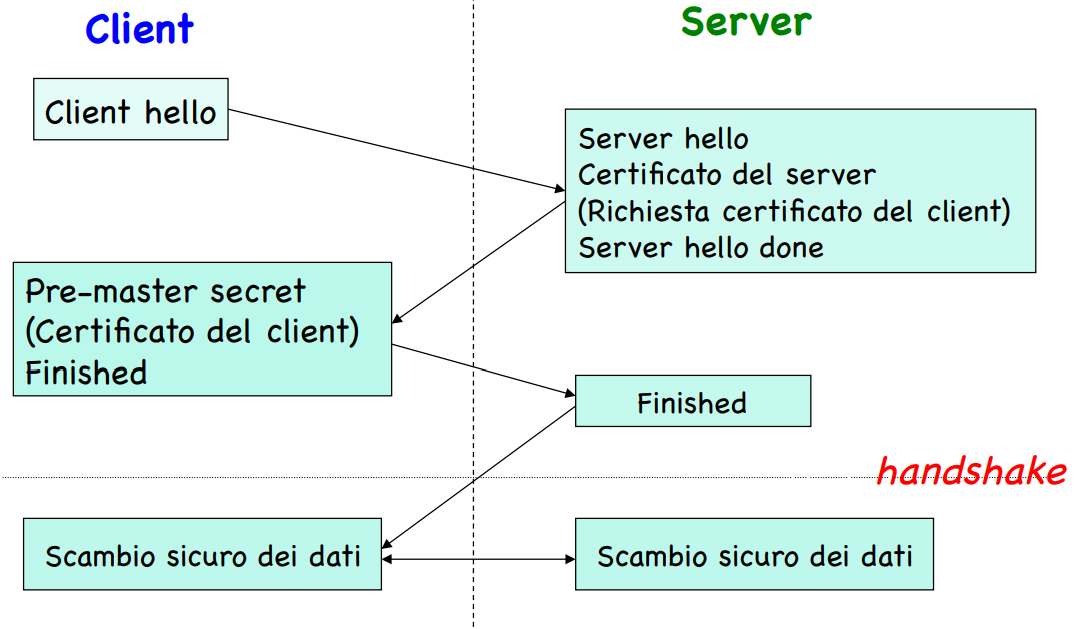
\includegraphics[scale=0.5]{20.png}
\end{center}
\paragraph{Sicurezza} Nei passi di \texttt{hello}, i due partner creano e si inviano due sequenze casuali per la costruzione del master secret, che risulta così diverso in ogni sessione SSL.\\
Il \textbf{crittoanalista non può riutilizzare i messaggi di handshake catturati sul canale per sostituirsi a S in una successiva comunicazione con U}.
\paragraph{MAC dei blocchi di dati} SSL record numera in modo incrementale ogni blocco di dati e autentica il blocco attraverso un MAC.\\
Per prevenire la modifica del blocco da parte di un crittoanalista attivo, il MAC viene calcolato come immagine hash one-way di una stringa costruita concatenando:
\begin{list}{}{}
	\item il contenuto del blocco
	\item il numero del blocco nella sequenza
	\item la chiave del MAC
	\item alcune stringhe note e fissate a priori
\end{list}
Dato che i MAC sono cifrati assieme al messaggio, un crittoanalista non può alterarli senza aver forzato la chiave simmetrica di cifratura: \textbf{un attacco volto a modificare la comunicazione tra i due partner è difficile almeno quanto quello volto alla sua decrittazione}.
\paragraph{Il sistema è autenticato} Il canale definito da SSL handshake è immune da attacchi attivi MitM poiché il sistema S viene autenticato con un certificato digitale.\\
L'utente U può comunicare il pre-master secret al sistema S in modo sicuro attraverso la chiave pubblica presente nel certficato di S.\\
\textbf{Solo S può decifrare quel crittogramma} e costruire il master secret, su cui si fonda la costruzione di tutte le chiavi segrete adottate nelle comunicazioni successive.\\
Solo il sistema S, quello a cui si riferisce il certificato, potrà quindi entrare nella comunicazione con l'utente U.
\paragraph{L'utente può essere autenticato} Il certificato di U, se richiesto, e la sua firma apposta sui messaggi scambiati nel protocollo (SSL history) consentono a S di verificare che U sia effettivamente quello che dichiara di essere e che i messaggi siano stati effettivamente spediti da esso.\\
Se ciò non si verifica, S deduce che il protocollo è stato alterato (casualmente o maliziosamente con un attacco MitM) e interrompe la comunicazione.\\
L'opzionalità della comunicazione ha reso l'SSL molto diffuso nelle transazioni commerciali via internet: per gli utenti, la necessità di certificazione può costituire un ostacolo pratico ed economico. L'utente può essere autenticato con altrim etodo (logi, pin\ldots)
\pagebreak
\paragraph{Generazione delle sequenze casuali} Le tre sequenze casuali generate da U e da S e comunicate nei messaggi di \texttt{client hello}, \texttt{server hello} e pre-master secret sono usate per creare il master secret, quindi per generare le chiavi segrete di sessione.
\begin{list}{}{}

	\item La sequenza corrispondente al pre-master secret viene
generata da U e comunicata per via cifrata a S.
	\item La non predicibilità di questa sequenza è cruciale per la
sicurezza del canale SSL:\\
	una sua cattiva generazione renderebbe il protocollo molto debole.
\end{list}
\paragraph{Messaggio \texttt{finished}} Contiene tutte le informazioni scambiate nel corso dell'handshake.\\
Scopo: consente un ulteriore controllo sulle comunicazioni precedenti per garantire che:
\begin{list}{}{}
	\item Queste siano avvenute correttamente
	\item U e S dispongano dello stesso master secret
	\item Che la comunicazione non sia stata oggetto di un attacco attivo
\end{list}
\paragraph{SSL} Almeno sicuro quanto il più debole cipher suite supportato. Dal 200 le norme internazionali non pongono alcuna limitazione sui cifrari impiegabili (se non il alcuni paesi).\\
Consigliato disabilitare i propri sistemi dall'impiego di cifrari ormai notoriamente insicuri e chiavi troppo corte.

\chapter{Esercizi}
\section{Complessità e randomizzazione}
\paragraph{Esercizio 1} Un sistema crittografico impiega chiavi private di 46 bit. Per decifrare un messaggio $m$ data la
chiave, un programma in assembler impiega un ciclo di 128 istruzioni ripetuto in media tante volte
quanti sono i bit che costituiscono $m$. Impiegando un calcolatore che esegue un'operazione
assembler in un tempo medio di 10 ns, indicare in ordine di grandezza quanti anni sarebbero
necessari in media per condurre un attacco esaustivo sulle chiavi per un messaggio m di 1000 bit.\\
Indicare i calcoli eseguiti.
\subparagraph{Svolgimento} \begin{list}{}{}
	\item \# chiavi = $2^{46}$
	\item \# operazioni per chiave = 128 $\cdot\:|m|$
	\item $|m| = 1000$ bit $= 10^3$ bit
	\item 1 ns = $10^{-9}$s
	\item $\Rightarrow t = 2^{46}\cdot128\cdot10^3\cdot10\cdot10^{-9}$s = $2^{46}\cdot2^7\cdot10^{-5}$s = $2^{53}\cdot10^{-5}$s = $2^3\cdot2^{50}\cdot10^{-5}$s e dato che $2^{10} \simeq 10^3$\\
	$\Rightarrow\:\simeq 2^8\cdot(10^3)^5\cdot10^{-5}$s = $8\cdot10^{10}$s $\simeq$ 2500 anni
\end{list}
\paragraph{Esercizio 2} Si vuole generare una sequenza di bit pseudocasuali utilizzando il generatore BBS basato sulla
legge: $$x_i = x_{i-1}^2\textsl{ mod }n\:\:\:\:\:b_i = 1 \Leftrightarrow x_{m-i}\textsl{ è dispari}$$
\begin{enumerate}
	\item \textbf{Scegliere} $n = 11\cdot23$ e verificare che 11 e 23 soddisfano i requisiti del BBS
	\item Sia M la propria matricola. Porre $y =$ M mod 100 e $x_0 = y^2$ mod $n$ e \textbf{indicare} una sequenza di 10 bit generati, riportando i calcoli
	\item \textbf{Discutere} se il generatore è crittograficamente sicuro
\end{enumerate}
\subparagraph{Svolgimento}
\begin{enumerate}
	\item Verificare che 11 mod 4 = 3 (ok) e 23 mod 4 = 3 (ok)\\
	Verificare che $2\lfloor\frac{11}{4}\rfloor + 1 = 2\cdot + 1 = 5$ e $2\lfloor\frac{23}{4}\rfloor + 1 = 11$ siano primi fra loro (sono primi entrambi, ok)
	\item Usiamo M = 123456, M mod 100 = 56 e 11$\cdot$23 = 253
	\begin{multicols}{2}
	\begin{list}{}{}
		\item $x_0$ = 56$^2$ mod 253 = 100 $\rightarrow$ 0
		\item $x_1$ = 100$^2$ mod 253 = 133 $\rightarrow$ 1
		\item $x_2$ = 133$^2$ mod 253 = 232 $\rightarrow$ 0
		\item $x_3$ = 232$^2$ mod 253 = 188 $\rightarrow$ 0
		\item $x_4$ = 188$^2$ mod 253 = 177 $\rightarrow$ 1
		\item $x_5$ = 177$^2$ mod 253 = 210 $\rightarrow$ 0
		\item $x_6$ = 210$^2$ mod 253 = 78 $\rightarrow$ 0
		\item $x_7$ = 78$^2$ mod 253 = 12 $\rightarrow$ 0
		\item $x_8$ = 12$^2$ mod 253 = 144 $\rightarrow$ 0
		\item $x_9$ = 144$^2$ mod 253 = 243 $\rightarrow$ 1
		\item $\longrightarrow$ 1000010010
	\end{list}
	\end{multicols}
\end{enumerate}
\pagebreak
\paragraph{Esercizio 3} Sia C una sequenza ottenuta rappresentando in binario ciascuna delle due cifre centrali del
numero di matricola del candidato, prendendo per ciascuna di esse i tre bit meno significativi,
concatenando questi due gruppi di bit e aggiungendo 1 in testa.
\begin{enumerate}
	\item Eseguire 37$^C$ mod 100 per esponenziazioni successive \textbf{indicando} i calcoli eseguiti
	\item \textbf{Spiegare} perché tale metodo di calcolo è considerato efficiente
\end{enumerate}
\subparagraph{Svolgimento} Con M = 123456, 3 = 011 e 4 = 100\\
C = 1011100 = 64 + 16 + 8 + 4 = 92
\begin{enumerate}
	\item 37$^{92}$ mod 100 = 37$^{64 + 16 + 8 + 4}$ mod 100
	\begin{list}{}{}
		\item 37$^{4}$ mod 100 = 69$^2$ mod 100 = \underline{61}
		\item 37$^{8}$ mod 100 = 61$^2$ mod 100 = \underline{21}
		\item 37$^{16}$ mod 100 = 21$^2$ mod 100 = \underline{41}
		\item 37$^{32}$ mod 100 = 41$^2$ mod 100 = 81
		\item 37$^{64}$ mod 100 = 81$^2$ mod 100 = \underline{61}
		\item $\Rightarrow$ 37$^{92}$ mod 100 = $(61\cdot41\cdot21\cdot61)$ mod 100 = 81
	\end{list}
	\item Perché esegue un numero di moltiplicazioni logaritmico nel valore dell'esponente (dunque lineare nella dimensione)
\end{enumerate}
\paragraph{Esercizio 4} 
Applicando l’algoritmo Miller-Rabin, individuare un numero N primo di tre cifre decimali con
probabilità di errore minore di $\frac{1}{50}$, spiegando il procedimento eseguito.
\subparagraph{Svolgimento} $N = 113$, ho $\frac{1}{4^k} < \frac{1}{50}$ per $k = 3$, quindi servono 3 testimoni $y$ scelti a caso $\in [2,112]$\\
Pongo $y = 3$
\begin{enumerate}
	\item MCD(113, 3) = MCD(3, 113 mod 3) = MCD(2, 3 mod 2) = MCD(1, 0) = 1 ok
	\item N = 113\\
	N-1 = 112 = 2$^4\cdot$7, $w = 4$ e $z = 7$\\
	$3^7$ mod 113 = $3^{1+2+4}$ mod 113 =
	\begin{list}{}{}
		\item $3^2$ mod 113 = 9
		\item $3^4$ mod 113 = 9$^2$ mod 113 = 81
	\end{list}
	= $(3\cdot 9 \cdot 81)$ mod 113 = 40 $\neq 1$, bisogna proseguire nella valutazione di P2\\
	$0 \leq i \leq w - 1 = 3$
	\begin{list}{}{}
		\item[$i = 0$] $3^{2^0\cdot7}$ mod 113 = $3^7$ mod 113 = 40 $\neq -1$ (40 preso dal precedente risultato)
		\item[$i = 1$] $3^{2^1\cdot7}$ mod 113 = $(3^7)^2$ mod 113 = 40$^2$ mod 113 = 18 $\neq -1$ (40 preso dal precedente risultato)
		\item[$i = 2$] $3^{2^2\cdot7}$ mod 113 = $(18)^2$ mod 113 98 $\neq -1$ (18 preso dal precedente risultato)
		\item[$i = 3$] $3^{2^3\cdot7}$ mod 113 = $(98)^2$ mod 113 -1 $= -1$ ok (98 preso dal precedente risultato)
	\end{list}
\end{enumerate}
Per gli altri 2 valori di $y$ il procedimento è analogo
\section{Cifrari Storici}
\paragraph{Esercizio 1} \textbf{Decifrare} i seguenti crittogrammi
\begin{enumerate}
	\item YMNXJCJWHNXJNXJFXD (Cifrario Cesare, chiave $k \neq 3$)
	\item REXETSIH ONSICESI UCIFTFID REHTLIET (Cifrario a permutazione semplice, $h = 8$)
\end{enumerate}
\subparagraph{Svolgimento}
\begin{enumerate}
	\item Con $k = 21$ diventa THISEXERCISEISEASY
	\item Con $\pi = \{5, 8, 7, 6, 4, 3, 2, 1\}$ diventa THISEXER CISEISNO TDIFFICU LTEITHER
\end{enumerate}
\pagebreak
\paragraph{Esercizio 2} Dato un cifrario affine (mod 26), si fa un attacco di tipo chosen plain-text usando il testo \textit{hahaha}. Il testo cifrato è \textit{nonono}. Determinare la funzione di cifratura.
\subparagraph{Svolgimento} Un cifrario affine è un cifrario che associa a pos(X) = $a\cdot$pos(Y) + $b$\\
Bisogna trovare $a,b$ $|$ pos(\textit{n}) = $a\cdot$pos(\textit{h}) + $b$ mod 26 $\wedge$ pos(\textit{o}) = $a\cdot$pos(\textit{a}) + $b$ mod 26\\con pos(\textit{n}) = 13, pos(\textit{h}) = 7, pos(\textit{o}) = 14 e pos(\textit{a}) = 0\\
$\left\{
\begin{array}{l}
	13 = a\cdot7+b\textsl{ mod }26 \Leftrightarrow a = 11\\
	14 = a\cdot0+b\textsl{ mod }26 \Leftrightarrow b = 14
\end{array}
\right.$ ottentendo i due parametri $a = 11$ e $b = 14$ che danno il cifrario\\pos(Y) = (11$\cdot$pos(X) + 14) mod 26
\paragraph{Esercizio 3} Se nei cifrari affini si lavorasse in modulo 27 invece che modulo 26, quante sarebbero le chiavi possibili? E in modulo 29?
\subparagraph{Svolgimento} Con un alfabeto di 27 caratteri, $a$ deve essere primo con 27 = $3^3$\\$\rightarrow$ $a$ può assumere i valori da 1 a 26 non multipli di 3\\$\longrightarrow$ $\phi$(27) = $\phi$($3^3$) = $2\cdot3^2$ = 18 (tramite la \textbf{funzione di Eulero} $\phi$($p^k$) = $(p-1)p^{k-1}$ con $p$ primo)\\
$\rightarrow$ $b$ può assumere tutti i valori $\in[0, 26]$\\
$\Rightarrow$ \# chiavi = 18$\cdot$27 - 1 = 485 (il -1 esclude la coppia $(a,b) = (1,0)$ che lascia invariato il messaggio)\\\\
Con un alfabeto di 29 caratteri: 29 è primo, quindi $a$ può assumere tutti i valori $\in [1, 28]$ ($\rightarrow \phi(29) = 28$) e $b$ tutti i valori $\in [0, 28]$\\
$\Rightarrow$ \# chiavi = $28\cdot29 - 1 = 811$
\paragraph{Esercizio 4} Questo esercizio ha lo scopo di dimostrare che un cifrario affine iterato ha la stessa sicurezza di un cifrario singolo.\\
Si considerino due cifrari affini:
\begin{list}{}{}
	\item $C_1(x) = (a_1\cdot x + b_1)$ mod 26
	\item $C_2(x) = (a_2\cdot x + b_2)$ mod 26
\end{list}
\textbf{Dimostrare} che $\exists$ un cifrario affine $C_3$ $|$ $C_3(x) = C_2(C_1(x))$
\subparagraph{Svolgimento}
$C_2(C_1(x)) = (a_2\cdot C_1(x) + b_2)$ mod 26 $= (a_2\cdot(a_1 + b_1) + b_2)$ mod 26\\$= (a_1a_2x + a_2b_1 + b_2)$ mod 26 $= (a_3\cdot x + b_3)$ mod 26\\
Con $a_3 = a_1a_2$ mod 26, $b_3 = a_2b_1 + b_2$ mod 26
\paragraph{Esercizio 5} Il crittogramma $c$ = MBR OJFGA SWNTE CNK QJDIL NURW MBR XHMR è ottenuto cifrando $m$ = THE QUICK BROWN FOX JUMPS OVER THE GATE con un cifrario a sostituzione monoalfabetica completo.
\begin{enumerate}
	\item Quanta informazione relativa alla chiave si può determinare conoscendo la coppia $m, c$?
	\item Quante chiavi differenti potrebbero essere state usate per cifrare il messaggio $m$?
	\item \textbf{Decifrare} il crittogramma MBR TRHLRP WHE HTHV CWND PNEYNE ZNN, che è stato cifrato usando la stessa chiave usata per cifrare $m$
\end{enumerate}
\subparagraph{Svolgimento}
\begin{enumerate}
	\item Parte della permutazione che definisce il cifrario.\\
	Più precisamente, si trova l'immagine cifrata di 22 caratteri su 26.
	\item 24 chiavi\\
	Infatti mancano le corrispondenze per 4 caratteri, e se ne potrebbero costruire 4! = 24 differenti
	\item THE WEASEL RUN AWAY FROM LONDON ZOO
\end{enumerate}
\pagebreak
\paragraph{Esercizio 6} Usando il metodo di Vigenère, \textbf{cifrare} il messaggio CRITTOGRAFIA impiegando come chiave le prime 4 lettere del proprio cognome. \textbf{Spiegare} inoltre come tale cifrario possa essere attaccano.
\subparagraph{Svolgimento} Si incrocia la lettera del messaggio con la lettera del crittogramma sulla tabella di Vigenère per trovare la lettera cifrata. Ad esempio, alla colonna C e riga M corrisponde la lettera O.
\begin{list}{}{}
	\item \texttt{C R I T T O G R A F I A}
	\item \texttt{M A T T M A T T M A T T}
	\item[$\rightarrow$] \texttt{O A B M F O Z K M F B T}
\end{list}
Per la spiegazione, vedi appunti.
\paragraph{Esercizio 7}
Si deve cifrare il messaggio APPELLODIFEBBRAIO impiegando come chiave una permutazione
arbitraria e segreta delle 26 lettere dell’alfabeto.
\begin{enumerate}
	\item \textbf{Mostrare} la permutazione scelta e il crittogramma ottenuto
	\item \textbf{Calcolare} il numero di prove necessarie per condurre un attacco esauriente sulle chiavi
	\item \textbf{Discutere} la possibilità di un attacco più efficiente confrontandolo con quello del punto 2
\end{enumerate}
\subparagraph{Svolgimento}
\begin{enumerate}
	\item Ad esempio, DOAIIPFAPEREBBLOL
	\item In generale 26! - 1\\
	Ma per decifrare il crittogramma ottenuto cifrando APPELLODIFEBBRAIO occorrono meno prove, perché il crittogramma contiene 10 lettere diverse tra loro da decifrare.\\
	$\Rightarrow$ \# prove = $26\cdot25\cdot\ldots\cdot17$ = $\frac{26!}{16!} \simeq 2\cdot10^{13}$
	\item Crittoanalisi statistica
\end{enumerate}
\section{Cifrari Perfetti}
\paragraph{Esercizio 1} Sia M il numero di matricola del candidato. Si converta M in una sequenza binaria B trasformando
ordinatamente in binario ogni cifra decimale di M, prendendo per ciascuna di esse i tre bit meno significativi e concatenando tali gruppi di tre bit.
\begin{enumerate}
	\item \textbf{Indicare} la sequenza B, \textbf{proporre} una chiave K di 18 bit ottenuta lanciando idealmente una moneta e \textbf{trasformare} B mediante One-Time Pad usando K
	\item \textbf{Spiegare} se il cifrario può ritenersi sicuro per messaggi binari di lunghezza multipla di 18, utilizzando come chiave una ripetizione di K per il numero di volte necessario
\end{enumerate}
\subparagraph{Svolgimento}
\begin{enumerate}
	\item B = \texttt{101011000010101111}\\
	K = \texttt{010111001110111011}\\
	C $\Rightarrow$ \texttt{111100001100010100}
	\item Il riutilizzo di K rende il procedimento indicato non sicuro quanto il one-time pad
\end{enumerate}
\paragraph{Esercizio 2} In un cifrario A esistono un messaggio $m$ e un crittogramma $c$ $|$ P(M = $m$) = $p \leq \frac{1}{4}$, P(C = $c$) = $1 - p$\\
\textbf{Spiegare} se A può essere un cifrario perfetto e le conseguenze per un crittoanalista per la coppia $m,c$ indicata.
\subparagraph{Svolgimento}
\paragraph{Esercizio 3} \textbf{Spiegare} con precisione matematica e proprietà di linguaggio perché il cifrario One-Time Pad su messaggi di $n$ bit non può essere ritenuto perfetto se la chiave non è scelta perfettamente a caso.
\subparagraph{Svolgimento} Se ho una chiave con una qualche regolarità, lo xor farebbe filtrare tale proprietà sul crittogramma.
\paragraph{Esercizio 4} Nel codice one-time pad si sostituisca $\oplus$ con $\vee$ o con $\neg\oplus$.\\
Spiegare, nei due casi, se il protocollo funziona con le stesse proprietà del codice originale.
\subparagraph{Svolgimento} 
\paragraph{Esercizio 5} Qual è lo svantaggio principale del cifrario one-time pad?
\subparagraph{Svolgimento} La chiave: deve essere perfettamente casuale e non venire riutilizzata.
\paragraph{Esercizio 6} Nel one-time pad si consideri una coppia arbitraria messaggio-crittogramma $m, c$ di $n$ bit.\\
\textbf{Spiegare} quanto vale P(M = $m$, C = $c$) (nota: è la probabilità dell'intersezione degli eventi, non quella condizionale)
\subparagraph{Svolgimento}
\section{Cifrari Simmetrici}
\paragraph{Esercizio 1} Sia C una sequenza ottenuta rappresentando in binario ciascuna delle due cifre centrali del
numero di matricola del candidato, prendendo per ciascuna di esse i tre bit meno significativi e concatenando questi due gruppi di tre bit. Nella fase $i$-esima del DES, C costituisca la parte iniziale della sequenza in ingresso della S-box
\begin{enumerate}
	\item \textbf{Indicare} la sequenza C
	\item \textbf{Indicare}, con interi crescenti da 1 a 32, la sequenza POS di posizioni dei bit di D[$i$] influenzati da C, \textbf{spiegando} com'è stato ottenuto il risultato
	\item Posto che la parte sinistra di S[$i-1$] del messaggio entrante nella fase $i$ sia una sequenza di 1, \textbf{indicare} il valore dei bit di D[$i$] di cui al punto 2, \textbf{riportando} i calcoli eseguiti
\end{enumerate}
\subparagraph{Svolgimento} \begin{enumerate}
	\item \texttt{000010}
	\item Passando attraverso $S_1$, C dà in output \texttt{0100} (prendo i due bit esterni \texttt{00} per l'indice $x$ e i rimanenti \texttt{0001} per l'indice $y$, trovando 04 nella tabella che in binario è \texttt{0100})\\
	Questi bit andranno rispettivamente in posizione 9, 17, 23 e 30 di D[$i$], seguendo la tabella P (01 è in posizione 9 e così via). Quindi D[9] = 0, D[17] = 1, D[23] = 0 e D[30] = 0
	\item Con S[$i-1$] eseguo lo $\oplus$ (xor) con i bit in uscita da P. Quindi D[9] = 1$\oplus$0 = 1, D[17] = 1$\oplus$1 = 0,\\D[23] = 1$\oplus$0 = 1 e D[30] = 1$\oplus$0 = 1
\end{enumerate}
\paragraph{Esercizio 2} Si trasformi il DES complementando tutte le uscite della s-box.\\
Sia $M$ il proprio numero di matricola. Si converta $M$ in una sequenza binaria $B$ trasformando ordinatamente in binario ogni cifra decimale di $M$ e prendendo per ciascuna i tre bit meno significativi. Si estenda $B$ fino ad avere 48 bit, aggiungendo zeri a destra: sia tale sequenza l'uscita del blocco EP del DES con chiave $k[0] = 1010\ldots10$
\begin{enumerate}
	\item \textbf{Indicare} la sequenza $B$
	\item Nella fase 1 del DES, \textbf{determinare} il valore dei primi 4 bit a sinistra in uscita dalla s-box, spiegando come è stato ottenuto il risultato
	\item \textbf{Commentare} se il DES così modificato appaia o meno palesemente meno sicuro della versione standard
\end{enumerate}
\subparagraph{Svolgimento}
\begin{enumerate}
	\item $B =$ \texttt{101 011 000 010 101 111 000 000 000 000 000 000 000 000 000 000}
	\item Nella $S_i$ entrano 6 bit, quindi per vedere i primi 4 bit prodotti bisogna usare la $S_1$ con i primi 6 bit di $B$, cioè con \texttt{1 0101 1}. Con i bit esterni si indicizza $x$, in questo caso con valore 3 uso la quarta riga, e con i 4 bit interni si indicizza $y$, in questo caso con valore 5, ottenendo il valore $09$, che quindi consiste nei bit \texttt{1001}. Per la modifica proposta, bisogna complementare ogni bit, ottenendo \texttt{0110}.
	\item
\end{enumerate}
\pagebreak
\paragraph{Esercizio 3} Nella fase $i$-esima del DES, siano \texttt{000011} i primi 6 bit a sinistra in ingresso alla s-box.
\begin{enumerate}
	\item \textbf{Indicare} (con interi crescenti tra 1 e 32) la sequenza POS di posizioni dei bit di S[$i+1$] influenzati da questi 6 bit, spiegando come è stato ottenuto il risultato.
	\item Siano $c_1 c_2\ldots$ i bit di S[$i-1$] nelle posizioni indicate in POS (le stesse quindi di S[$i+1$]). $c_1 c_2\ldots$ rappresentino in binario il numero di consonanti presenti nel nome e cognome del candidato. \textbf{Indicare} il valore dei bit di S[$i+1$] nelle posizioni POS spiegando come è stato ottenuto il risultato.
\end{enumerate}
\subparagraph{Svolgimento}
\begin{enumerate}
	\item Avendo \texttt{1 0001 1} come bit, ottengo 12 cioè \texttt{1100} come bit.\\
	Ogni bit andrà, secondo la tabella P, rispettivamente in posizione 9, 17, 23, 31 di D[$i$], che diventerà S[$i+1$].
	\item La sequenza data da $c$ è \texttt{1000}.\\
	Bisogna fare lo $\oplus$ tra S[$i-1$] = \texttt{1000} e D attuale = \texttt{1100}. Quindi
	\begin{list}{}{}
		\item S[9] = $1\oplus1 = 0$
		\item S[17] = $0\oplus1 = 1$
		\item S[23] = $0\oplus0 = 0$
		\item S[31] = $0\oplus0 = 0$
	\end{list}
	ottenendo \texttt{0 1 0 0} rispettivamente nelle posizioni 9, 17, 23, 31.
\end{enumerate}
\paragraph{Esercizio 4} La s-box del cifrario AES è composta da 16 blocchi con 8 ingressi e 8 uscite ciascuno. Qual è il numero totale di possibili funzioni che si potrebbero scegliere per costruire ciascun blocco?
\subparagraph{Svolgimento} Per ognuna delle $2^8$ configurazioni di input, posso scegliere $2^8$ configurazioni in output. Quindi ho \# funzioni = $\left(2^8\right)^{2^8}$ = $2^{8\cdot2^8}$
\paragraph{Esercizio 6} La proprietà di non linearità di qualsiasi cifratura a blocchi è fondamentale per la sicurezza. Infatti, si supponga di avere una cifratura lineare a blocchi $Cl$ che figra blocchi di 128 bit di testo in chiaro in 128 bit di testo cifrato, usando una chiave $k$ la cui lunghezza è irrilevante. Dunque, ogni coppia di messaggi $m_1$ e $m_2$ risulta $Cl(m_1\oplus m_2, k) = Cl(m_1, k)\oplus Cl(m_2, k)$\\
\textbf{Descrivere} come un avversario che abbia 128 testi cifrati scelti possa decifrare qualsiasi testo cifrato senza conoscere la chiave $k$.
\subparagraph{Svolgimento} Prendo $c$ il crittogramma di un generico $m$, $c = Cl(m, k)$. Posso rappresentare $c = \bigoplus_{i:c_i = 1} e^{(i)}$ dove $e_{(i)}$ ha un solo bit a 1 in posizione $i$, e gli altri 127 bit a 0.\\
Per esempio $c = 1011 = 1000\oplus0010\oplus0001 = e^{(1)}\oplus e^{(3)}\oplus e^{(4)}$\\
Sfruttiamo le proprietà delle funzioni di cifratura e decifrazione: $m = D(c,k) = D(\bigoplus_{i:c_i = 1} e^{(i)}, k) = \bigoplus_{i:c_i = 1} D(e^{(i)}, k)$\\
Si chiede la decifrazione dei 128 testi cifrati $e^{(i)}$, $i\in[1,128]$, $f^{(i)} = D(e^{(i)}, k)$\\
Si può decifrare qualsiasi crittogramma $c$ anche senza conoscere $k$: $m = \bigoplus_{i:c_i = 1}f^{(i)}$
\paragraph{Esercizio 7} DESX è un cifrario proposto da Rivest per proteggere il DES dagli attacchi esaurienti. DESX usa una chiave segreta $w$ di 64 bit, oltre alla chiave DES $k$ di 56 bit, e opera così: $$C_{DESX}(m, k, w) = w\oplus C_{DES}(m\oplus w, k)$$Mostrare come eseguire la decifrazione.
\subparagraph{Svolgimento}
$c = C_{DES}(m\oplus w, k) \Leftrightarrow c\oplus w = C_{DES}(m\oplus w, k)$\\
$\Leftrightarrow D_{DES}(c\oplus w, k) = D_{DES}(C_{DES}(m\oplus w, k))$ ma $D_{DES}(C_{DES}(m\oplus w, k)) = m\oplus w$ perché DES è un cifrario corretto\\
Quindi $\Leftrightarrow m\oplus w = D_{DES}(c\oplus w, k) \Leftrightarrow m = w \oplus D_{DES}(c\oplus w, k)$
\section{Cifrari Asimmetrici}
\paragraph{Esercizio} \begin{enumerate}
	\item \textbf{Spiegare} in cosa consiste il cifrario RSA e \textbf{dimostrarne} la correttezza.
	\item \textbf{Darne un esempio} di applocazione impiegando parametri numerici molto piccoli per cifrare il messaggio costituito dalle due cifra meno significative del proprio numero di matricola.
\end{enumerate}
\subparagraph{Svolgimento} \begin{enumerate}
	\item Si basa sulla moltiplicazione di due numeri primi, facile da eseguire ma difficile da invertire, e fa uso dell'algebra modulare che rende difficili alcuni problemi facili nell'algebra non modulare.\\
	Scelti $p,q$ primi, la cifratura è eseguita con la chiave pubblica del destinatario, $k_{pub}$ composta da $e < (p-1)(q-1)$ coprimo con $n = pq$ e da $n$. La decifrazione è fatta dal destinatario con la proprio chiave privata $k_{priv} = d = e^{-1}$ mod $(p-1)(q-1)$. Vedi p. 43.
	\item Usando $p = 3$, $q = 5$, cifro $m = 13$\\
	$n = 15$, $\phi(n) = (p-1)(q-1) = 2\cdot4 = 8$ quindi posso scegliere $e = 7$ che rispetta le condizioni.\\
	$d = 7^{-1}$ mod $8 = 7$ perché $7\cdot 7$ mod $8 = 49$ mod $8 = 1$\\
	$c = C(m, k_{pub}) = m^e$ mod $n = 13^7$ mod $15 = 7$\\
	$m = D(c, k_{priv}) = c^d$ mod $n = 7^7$ mod $15 = 13$
\end{enumerate}
\paragraph{Esercizio 2} Poniamo che si scopra un algoritmo polinomiale per calcolare la funzione di Eulero. \textbf{Spiegare} in termini matematici quale influenza la scoperta avrebbe sul cifrario RSA.
\subparagraph{Svolgimento} Si potrebbe calcolare in tempo polinomiale la chiave privata $d = e^{-1}$ mod $\phi(n)$. Il cifrario sarebbe compromesso e non più utilizzabile.
\paragraph{Esercizio 3} Per la costruzione di una coppia di chiavi RSA si sceglie $n$ come prodotto di due primi $p,q$ considerando le seguenti possibilità:\begin{enumerate}
	\item$p=\Theta(n^{1/2}),q=\Theta(n^{1/2})$
	\item$p=O(n^{1/3}),q=O(n^{2/3})$
	\item$p=\Theta(n^{1/3}),q=\Theta(n^{1/3})$
	\item$p=O(\log n),q=O(n/\log n)$
\end{enumerate}
Per ciascuna di queste possibilità, \textbf{spiegare} con precisione se la scelta è corretta e consigliabile.
\subparagraph{Svolgimento} \begin{enumerate}
	\item No, $p,q$ troppo vicini
	\item Ok, $p,q$ sufficientemente grandi e distanti tra loro
	\item No, $p\cdot q$ non è $\Theta(n)$
	\item $p$ troppo piccolo, bruteforce avrebbe costo polinomiale
\end{enumerate}
\paragraph{Esercizio 4} Si consideri un cifrario RSA con $p = 7, q = 11, e = 13$
\begin{enumerate}
	\item \textbf{Determinare} il valore di $d$ chiave privata
	\item Qual'è la dimensione dei blocchi per la cifratura?
	\item \textbf{Cifrare} \texttt{100011001010}
\end{enumerate}
\subparagraph{Svolgimento} \begin{enumerate}
	\item $n = 77$, $\phi(n) = 60$, quindi $d = 13^{-1}$ mod $60 = 37$
	\item I blocchi saranno di $b = \lfloor\log_2 n\rfloor = 6$ bit
	\item Diviso in blocchi, $m =$ \texttt{100011 001010}, cioè cifro $m_1 = 35$ e $m_2 = 10$\\
	$c_1 = m_1^e$ mod $n = 35^{13}$ mod $77 = 63$\\
	$c_2 = m_2^e$ mod $n = 10^{13}$ mod $77 = 10$
\end{enumerate}
\pagebreak
\paragraph{Esercizio 5} Si consideri un cifrario RSA con chiave pubblica $n = 55, e = 7$
\begin{enumerate}
	\item \textbf{Cifrare} $m = 10$
	\item \textbf{Forzare} il cifrario trovando $p,q,d$
	\item \textbf{Decifrare} $c = 35$
\end{enumerate}
\subparagraph{Svolgimento} \begin{enumerate}
	\item $c = m^e$ mod $n = 10^7$ mod $55 = 10$
	\item $n = 55$ è il prodotto tra $p = 5$ e $q = 11$ quindi $\phi(55) = (p-1)(q-1) = 4\cdot 10 = 40$ e $d = 7^{-1}$ mod $40 = 23$
	\item $m = c^d$ mod $n = 35^{23}$ mod $55 = 30$
\end{enumerate}

\paragraph{Esercizio 6} Siano $x,y,n$ tre interi positivi arbitrari con $x,y < n$. Poniamo che si scopra un algoritmo di algebra modulare di complessità $O(d^2)$ per calcolare, se esiste, il logaritmo discreto di $y$ in base $x$ modulo $n$, con $d = \Theta(n)$ oppure $d = \Theta(\log n)$.\\
\textbf{Spiegare} in termini matematici, per i due suddetti valori di $d$, quale influenza la scoperta potrebbe avere sull'algoritmo DH per lo scambio segreto delle chiavi.
\subparagraph{Svolgimento} Il crittoanalista potrebbe arrivare a conoscere $A = g^x$ mod $p$ con $g$ generatore di $Z_p^*$, o analogamente $B = g^y$ mod $p$.\\
Avere un algoritmo efficiente per la risoluzione permetterebbe di trovare $x$ o $y$ in modo efficiente e renderebbe DH vulnerabile ad attacchi passivi.\begin{list}{}{}
	\item[$d=\Theta(n)$] L'algoritmo ha complessità esponenziale nella dimensione dell'input (polinomiale solo nel \textit{valore} di $n$). Nessuna influenza su DH che si può sempre usare in sicurezza
	\item[$d=\Theta(\log n)$] L'algoritmo è effettivamente polinomiale, quindi il protocollo DH non è più utilizzabile.
\end{list}
\paragraph{Esercizio 7} Si consideri il protocollo basato sull'algoritmo DH con $g=3, p=353$ e siano $x=97,y=233$. Calcolare $X,Y,k$
\subparagraph{Svolgimento}
\begin{list}{}{}
	\item $X = g^x$ mod $p = 3^{97}$ mod $353 = 40$
	\item $Y = g^y$ mod $p = 3^{233}$ mod $353 = 248$
	\item \texttt{k[session]} $= g^{xy}$ mod $p = 3^{97\cdot233}$ mod $p = 160$
\end{list}
\paragraph{Esercizio 8} Due utenti A e B vogliono costruire una chiave segreta di sessione impiegano il protocollo basato sull'algoritmo DH. A tale scopo concordano su una coppia pubblica di interi $p=11,g=6$
\begin{enumerate}
	\item \textbf{Dimostrare} che la coppia $\langle11,6\rangle$ è adatta per il protocollo DH
	\item Posto che A,B scelgano come numeri casuali segreti $x,y$ la quarta e quinta cifra della matricola del candidato, \textbf{creare} \texttt{k[session]} \textbf{indicando i calcoli eseguiti da A e B}
\end{enumerate}
\subparagraph{Svolgimento}
\begin{multicols}{2}
\begin{enumerate}
	\item $p,g$ proposti pari a $p=11$ e $g=6$, sono adatti perché $p$ è primo e $g$ è un generatore di $Z_{11}^* = \{1,2,\ldots, 10\}$\\$= \{6^k$ mod $11\:|\:1\leq k \leq 10\}$
	\begin{multicols}{2}
	\begin{list}{}{}
		\item[$k=1$] $6^1$ mod $11$ = 6
		\item[$k=2$] $6^2$ mod $11$ = 3
		\item[$k=3$] $6^3$ mod $11$ = 7
		\item[$k=4$] $6^4$ mod $11$ = 9
		\item[$k=5$] $6^5$ mod $11$ = 10
		\item[$k=6$] $6^6$ mod $11$ = 5
		\item[$k=7$] $6^7$ mod $11$ = 8
		\item[$k=8$] $6^8$ mod $11$ = 4
		\item[$k=9$] $6^9$ mod $11$ = 2
		\item[$k=10$] $6^{10}$ mod $11$ = 1
	\end{list}
	\end{multicols}
	\item A sceglie $x = 2$ e B sceglie $y = 5$\\
	A calcola $X = 6^2$ mod $11 = 3$, B calcola $Y = 6^5$ mod $11 = 10$ e se li scambiano.\\
	A calcolerà \texttt{k[session]} $= Y^x$ mod $p$ e B calcolerà \texttt{k[session]} $= X^y$ mod $p$\\
	In entrambi i casi, \texttt{k[session]} = $g^{xy}$ mod $p = 6^{10}$ mod $11 = 1$
\end{enumerate}
\end{multicols}
\pagebreak
\paragraph{Esercizio 9} Considerando il cifrario RSA:
\begin{enumerate}
	\item Discutere se è possibile scegliere un valore pari di $e$
	\item Siano $e,e'$ due valori scelti per la chiave pubblica tali che $e'$ è ottenuto da $e$ cambiando un bit da 0 a 1. Dimostrare che MCD$(e,e')=1$
\end{enumerate}
\subparagraph{Svolgimento} \begin{enumerate}
	\item $e$ pari significa $e = 2\cdot f$ con $f$ dispari.\\
	Dato che $\phi(n)$ è ottenuto con il prodotto $(p-1)(q-1)$ con $p,q$ primi, ho che entrambi i fattori sono pari, diciamo $p-1 = 2r, q-1=2s$, di conseguenza avrò MCD($2f, 4rs$) = 2 $\neq 1$
	\item Sia $e' = e + 2^i$ ($i$-esimo bit di $e$ è 0)\\
	$\forall\:t\:|\:\:\: t\:|\:e$ sappiamo che $t\neq 2$ (vedi punto 1), dunque $t\not|\:2^i$\\
	$\Rightarrow\forall\:t\:\:\:t\:|\:e,t\not|\:e'\Rightarrow$ MCD$(e,e') = 1$
\end{enumerate}
\paragraph{Esercizio 10} Nonostante il cifrario RSA sia sicuro, alcune sue implementazioni possono rendere insicura la cifratura. Si consideri ad esempio la cifratura di un messaggio $m$ di 64 bit con una chiave pubblica RSA $\langle e,n\rangle$ dove $e=3$ e $n$ è un numero da 512 bit.\begin{enumerate}
	\item \textbf{Spiegare} perché la cifratura di $m$ è completamente insicura
	\item \textbf{Decifrare} il crittogramma $c = 33076161$ con $n = 100082119$
\end{enumerate}
\subparagraph{Svolgimento} \begin{enumerate}
	\item Il motivo principale è che $n$ ha troppi pochi bit ed è attualmente fattorizzabile in tempi molto brevi.\\
	Inoltre, un messaggio $m$ da 64 bit con $e=3$ non viene ridotto in modulo per un $n$ da 512 bit ($m^e$ ha $64\cdot3=192$ bit). Avrò sempre $c = m^3$.
	\item $d = 3^{-1}$ mod $\phi(100082119)$, ma è inutile dato che il messaggio $m$ non è ridotto in modulo, posso direttamente calcolare $m = \sqrt[e]{c} = \sqrt[3]{33076161} = 321$
\end{enumerate}
\paragraph{Esercizio 11} Supponiamo che Eve intercetti il crittogramma $c = m^e$ mod $n$ diretto ad Alice. Si supponga inoltre che Alice sia disposta a decifrare per Eve qualsiasi crittogramma $c'$, a patto che $c'\neq c$.\\
\textbf{Descrivere} come Eve possa decifrare $m$ in tempo polinomiale, richiedendo ad Alice la decifrazione del crittogramma $c' = cx^e$ dove $x<n$ è un intero casuale coprimo con $n$.
\subparagraph{Svolgimento} Avendo $c' = cx^e = m^ex^e$ mod $n$ e $c = m^e$ mod $n$, ho $m' = (m^e)^d(x^e)^d$ mod $n = mx$,\\da cui ottengo $m = m'x$ mod $n$
\paragraph{Esercizio 12} Alice vuole mandare un messaggio cifrato a Bob usando RSA, ma non conosce la chiave pubblica. Invia una mail a Bob chiedendogliela, che risponde inviando $K_{pub} = \langle e,n\rangle$.\\
Eve intercetta il messaggio, sostituisce $e$ con un nuovo intero $e'$ coprimo con $e$, e invia la chiave modificata $k'_{pub} = \langle e',n\rangle$ ad Alice.\\
Alice usa $k'_{pub}$ per cifrare $m$, e invia il crittogramma $c' = m^{e'}$ mod $n$ a Bob.\\
Dato che $m$ è stato cifrato con la chiave sbagliata, Bob rimanda la propria chiave pubblica ad Alice che risponderà con il crittogramma corretto $c = m^e$ mod $n$.\\
\textbf{Mostrare} come Eve, che conosce $e,e',c,c'$, possa risalire a $m$.
\subparagraph{Svolgimento} $e,e'$ sono coprimi. Applicando EE (Euclide Esteso) si possono calcolare in tempo polinomiale $r,s\:|\:e\cdot r + e'\cdot s =$ MCD$(e,e')=1$\\
$\Rightarrow m = m^{er+e's}$ mod $n = (m^{er}$ mod $n)\cdot(m^{e's}$ mod $n)$ mod $n = c^r(c')^s$ mod $n$\\
Supponendo $r<0,s>0 \Rightarrow m = (c^{-1})^{-r}(c')^s$ mod $n$\\Eve calcola l'inverso di $c$, calcola $(c^{-1})^{-r}$ ($-r$ è positivo), calcola $(c')^s$ e ottiene $m$ dal loro prodotto ridotto in modulo.\\
Tutti i passaggi richiedono tempo polinomiale. L'inverso di $c$ modulo $n$ esiste ed è unico se $c,n$ sono coprimi. Se non lo fossero, Eve potrebbe allora fattorizzare $n$ e forzare il cifrario.
\pagebreak
\section{Funzioni hash, MAC e Firma digitale}
\paragraph{Esercizio 1} Spiegare che proprietà devono possedere le funzioni hash one-way e perché tali funzioni sono importanti nei protocolli di autenticazione e firma.
\subparagraph{Svolgimento} Una funzione hash one-way deve essere \textbf{facile da calcolare}, \textbf{difficile da invertire} e \textbf{difficile trovare due elementi che collidono}.
\paragraph{Esercizio 2} Si scriva un messaggio a piacere in italiano $m = m_{20}m_{19}\ldots m_0$ costituito da 21 caratteri alfabetici più lo spazio.\\
Si consideri il sottoinsieme dell'alfabeto $C_0 = \{A,B,\ldots,L\}$.\\
Utilizzando la chiave $k = k_5k_4k_3k_2k_1k_0$ consistente nelle 6 cifre decimale della propria matricola, si autentichi $m$ mediante il MAC di 6 bit $A(m,k) = h_5h_4h_3h_2h_1h_0$ costruito come segue:
\begin{lstlisting}
	j = 0
	for (i = 0 to 5) do
		j = k[i] + j mod 21
		if (m[j] in C0) then h[i] = 0 else h[i] = 1
\end{lstlisting}
\begin{enumerate}
	\item \textbf{Riportare} i valori di $m$ e $h_i$ per $i = 0,1,\ldots,5$ indicando i calcoli
	\item \textbf{Spiegare} se la funzione $A$ definita sopra è adatta per l'applicazione considerata.
\end{enumerate}
\subparagraph{Svolgimento} \begin{enumerate}
\item $m =$ \texttt{messaggio celatissimo}, $k =$ \texttt{530257}\begin{list}{}{}
	\item[$i=0$] $j = 7 + 0$ mod $21 = 7$, $m_7 = a \Rightarrow h_0 = 0$
	\item[$i=1$] $j = 5 + 7$ mod $21 = 12$, $m_{12} = o \Rightarrow h_1 = 1$
	\item[$i=2$] $j = 2 + 12$ mod $21 = 14$, $m_{14} = g \Rightarrow h_2 = 0$
	\item[$i=3$] $j = 14 + 0$ mod $21 = 14$, $m_{14} = g \Rightarrow h_3 = 0$
	\item[$i=4$] $j = 3 + 14$ mod $21 = 17$, $m_{17} = s \Rightarrow h_4 = 1$
	\item[$i=5$] $j = 5 + 17$ mod $21 = 1$, $m_1 = m \Rightarrow h_5 = 1$
	\item[$\Rightarrow$] $A(m,k) =$ \texttt{110010}
\end{list}
\item
\end{enumerate}
\pagebreak
\paragraph{Esercizio 3} Sia $S$ la somma delle sei cifre decimali del numero di matricola del candidato. Sia monga $M = S + 10$.\\
Si convertano le cifre di $M$ in binario su 4 bit, se le calcoli lo XOR e si riconverta il valore ottenuto in un numero decimale $H$ che sarà usato come hash di $M$: $h(M) = H$\\
Per due utenti Alice e Bob di un sistema RSA, si considerino i seguenti parametri:
\begin{list}{}{}
	\item Alice: $p=5,q=11,e=7,d=23$
	\item Bob: $p=7,q=13, e=5, d=29$
\end{list}
Alice deve spedire a Bob il messaggio $M$ cifrato e firmato in hash, impiegando le chiavi RSA e la funzione hash di cui sopra.
\begin{enumerate}
	\item \textbf{Spiegare} se i parametri RSA indicati sopra sono scelte in modo consistente con le regole del cifrario (a parte le dimensioni)
	\item \textbf{Indicare} esplicitamente tutte le operazioni aritmetiche fatte da Alice e Bob nella trasmissione e verifica del messaggio $M$ e della firma.
\end{enumerate}
\subparagraph{Svolgimento} 
\begin{enumerate}
	\item Per entrambi, abbiamo $p,q$ primi ed $e$ coprimo con $\phi(pq) = (p-1)(q-1)$:
	\begin{list}{}{}
		\item MCD($7, 40$) = 1
		\item MCD($5, 72$) = 1
	\end{list}
	Inoltre $23 = 7^{-1}$ mod $40$ e $29 = 5^{-1}$ mod $72$\\
	Quindi i valori sono appropriati a meno delle dimensioni.
	\item Usando il protocollo 3 \begin{list}{}{}
		\item \textbf{Alice}\\
		$M = 22 + 10 = 32 \rightarrow$ $H=$ \texttt{0011$\oplus$0010} $=$ \texttt{0001} $\rightarrow h(32) = 1$\\
		Calcola il crittogramma $c_m = 32^{5}$ mod $91 = 2$ con la chiave pubblica di Bob\\
		Calcola il crittogramma $c_H = 1^{23}$ mod $55 = 1$ con la propria chiave privata\\
		Spedisce $c_m$ e $c_H$ a Bob
		\item \textbf{Bob}\\
		Riceve $c_m$ e calcola $m = 2^{29}$ mod $91 = 32$ con la propria chiave privata\\
		Riceve $c_H$ e calcola $H_{Alice} = 1^{7}$ mod $55 = 1$ con la chiave pubblica di Alice\\
		Calcola $H$ con il precedente calcolo, lo verifica con $H_{Alice}$ ricevuto e conclude che il messaggio è autenticato.
	\end{list}
\end{enumerate}
\paragraph{Esercizio 4} Posto che si scopra un algoritmo polinomiale per calcolare la funzione di Eulero, \textbf{spiegare} in termini matematici quale influenza la scoperta avrebbe sui protocolli di firma.
\subparagraph{Svolgimento} Come per l'RSA, la scoperta di un algoritmo polinomiale per calcolare $\phi(n)$ si potrebbe calcolare in tempo polinomiale $d = e^{-1}$ mod $\phi(n)$, rendendo chiunque capace di firmare al posto dell'utente.
\paragraph{Esercizio 5} Sia $n = pq$ con $p,q$ primi, e sia $e$ un intero coprimo con $\phi(n)$. Si discuta se la funzione\\ $h(m_1,m_2) = m_1^em_2^e$ mod $n$ è resistente alle collisioni.
\subparagraph{Svolgimento} Non è resistente. Per dimostrarlo si prende $(m_1',m_2')=(m_2,m_1)$ e si ottiene una collisione con la coppia $(m_1,m_2)$, per la transitività della moltiplicazione.

\pagebreak
\paragraph{Esercizio 6} Due utenti A e B di un sistema RSA hanno scelto le seguenti chiavi: \texttt{k[pubA] = }$\langle 7,341\rangle$, \texttt{k[privA] = }$\langle43\rangle$, \texttt{k[pubB] = }$\langle5,299\rangle$, \texttt{k[privB] = }$\langle53\rangle$.\\
A deve mandare a B il seguento messaggio $m$ cifrato e firmato in hash, impiegando RSA e la seguente funzione hash $h$:
\begin{list}{}{}
	\item $m$ = numero di matricola del candidato, diviso in 3 blocchi $m_1,m_2,m_3$ di due cifra ciascuno
	\item $h(m) = (m_1+m_2+m_3)$ mod $100$
\end{list}
\begin{enumerate}
	\item Spiegare se le chiavi di A e B sono scelte in modo consistente con le regole del cifrario (a parte le loro dimensioni), elencando i calcoli eseguiti.
	\item Indicare esplicitamente tutte le operazioni aritmetiche eseguite da A e B nella trasmissione e verifica del messaggio $m$ e della firma.
\end{enumerate}
\subparagraph{Svolgimento} \begin{enumerate}
	\item \begin{list}{}{}
		\item[A] $n = 341 = pq = 11\cdot31 \Rightarrow \phi(n) = 300$\\
	MCD$(7, 300) = 1$ OK\\
	$d = 7^{-1}$ mod $300 = 43$ OK
	\item[B] $n = 299 = pq = 13\cdot23 \Rightarrow \phi(n) = 264$\\
	MCD$(5, 264) = 1$ OK\\
	$d = 5^{-1}$ mod $264 = 53$ OK
	\end{list}
	\item $m_1 = 53, m_2 = 02, m_3 = 57$\\
	\textbf{Firma e Cifratura}\\
	A calcola $h(m) = 53+2+57$ mod $100 = 14$\\
	A calcola la firma $f = D(h(m),$ \texttt{k[privA]}$) = 14^{43}$ mod $341 = 214$\\
	A calcola i crittogrammi $c_i = C(m_i,$ \texttt{k[pubB]}$) \Rightarrow \begin{array}{l}
	c_1 = m_1^e\textsl{ mod }299 = 53^5\textsl{ mod }299 = 40\\
	c_2 = m_2^e\textsl{ mod }299 = 2^5\textsl{ mod }299 = 32\\
	c_3 = m_3^e\textsl{ mod }299 = 57^5\textsl{ mod }299 = 5\\
	\end{array}$\\
	\textbf{Decifrazione e verifica}\\
	B decifra i crittogrammi $m_i = D(c_i$ \texttt{k[privB]}$) \Rightarrow \begin{array}{l}
	m_1 = c_1^d\textsl{ mod }299 = 40^{53}\textsl{ mod }299 = 53\\
	m_2 = c_2^d\textsl{ mod }299 = 32^{53}\textsl{ mod }299 = 2\\
	m_3 = c_3^d\textsl{ mod }299 = 5^{53}\textsl{ mod }299 = 57\\
	\end{array}$\\
	B calcola $h(m) = (m_1+m_2+m_3)$ mod $100 = 14$\\
	B verifica che $14 = C(f,$\texttt{k[pubA]}$) = 214^7$ mod $341 = 14$
\end{enumerate}
\paragraph{Esercizio 8}Si presenta un primo tentativo di firma elettronica basato su curve ellittiche. Si ha una curva ellittica globale, un numero primo $p$ e un \textit{generatore} B. Alice sceglie una chiave di firma privata $x_A$ e crea la chiave pubblica di verifica $Y_A = x_AB$. Per firmare il messaggio $M$:
\begin{list}{}{}
	\item Alice sceglie un valore $k$
	\item Alice invia a Bob $M,k$ e la firma $F = M - kx_AB$
	\item Bob verifica che $M = F + kY_A$
\end{list}
\begin{enumerate}
	\item Dimostrare che questo schema funziona correttamente. Ovvero, che il processo di verifica produce un'uguaglianza quando la firma è valida.
	\item Dimostrare che lo schema è inaccettabile descrivendo una semplice tecnica per creare la firma falsa di un utente su un qualsiasi messaggio.
\end{enumerate}
\subparagraph{Svolgimento} \begin{enumerate}
	\item $M = F + kY_A = M - kx_AB + kY_A = M - \not kx_AB + \not k(x_AB) = M$
	\item $F = M - kx_AB = M - kY_A$\\
	$k$ viene scelto da chi firma, e $Y_A$ è la chiave \textbf{pubblica} di chi firma
\end{enumerate}
\pagebreak
\paragraph{Esercizio 9} Si presenta un tentativo di firma elettronica basato su curve ellittiche. Si ha una curva ellittica globale, un numero primo $p$ e un \textit{generatore} B. Alice sceglie una chiave di firma privata $x_A$ e crea la chiave pubblica $Y_A = x_AB$. Per firmare un messaggio $M$:
\begin{list}{}{}
	\item Bob sceglie un valore $k$
	\item Bob invia ad alice $C = kB$
	\item Alice invia a Bob $M$ e la firma $F = M - x_AC$
	\item Bob verifica che $M = F + kY_A$
\end{list}
\begin{enumerate}
	\item Dimostrare che questo schema funziona correttamente. Ovvero, che il processo di verifica produce un'uguaglianza quando la firma è valida.
	\item Dimostrare che falsificare una firma con questo schema è difficile quanto forzare la crittografia a curva ellittica El Gamal
\end{enumerate}
\subparagraph{Svolgimento} \begin{enumerate}
	\item $M = F + kY_A = M - x_AC + kY_A = M - \not x_AkB + \not kx_AB = M$
	\item Per falsificare la firma bisogna calcolare $x_AC = x_A k B = k Y_A$\\
	$Y_A$ pubblico, ma $k$ non è noto. Per ricavarlo da $C = kB$ occorre risolvere il logaritmo discreto su curve ellittiche.\\
	L'alternativa consiste nel calcolare la chiave privata $x_A$ da $Y_A$, per cui occorre di nuovo risolvere il problema del logaritmo discreto su curve ellittiche.
\end{enumerate}
\section{Curve Ellittiche}
\paragraph{Esercizio 1} Il punto P = (4,7) appartiene alla curva ellittica $y^2 = x^3 - 5x + 5$ sui numeri reali?
\subparagraph{Svolgimento} Verificare se $7^2 = 4^3 - 5\cdot4 + 5 \Leftrightarrow 49 = 64-20+5 \Leftrightarrow 49 = 49$, quindi P appartiene alla curva
\paragraph{Esercizio 2} Nella curva ellittica sui reali $y^2 = x^4 - 36x$, siano P = (-3,9) e Q = (-2,8).\\
Trovare P + Q, 2P.
\subparagraph{Svolgimento}\begin{list}{}{Formule a p.48} 
	\item $P + Q = S = (x_s, y_s)$ con $\left\{\begin{array}{l}
		x_s = \left(\frac{9-8}{-3+2}\right)^2 + 3 + 2 = 6\\
		y_s = -9 + \left(\frac{9-8}{-3+2}\right)\left(-3-x_s\right) = -9 + (-1)(-9) = 0
	\end{array}\right. = (6,0)$
	\item $2P = T = (x_t, y_t)$ con $\left\{\begin{array}{l}
	x_t = \left(\frac{27 - 36}{18}\right)^2 + 3 + 3 = \frac{25}{4}\\
	y_t = -9 + \left(\frac{27 - 36}{18}\right)(-3-x_t)= -\frac{35}{8} 
	\end{array}\right. = \left(\frac{25}{4},-\frac{35}{8}\right)
	$
\end{list}
\paragraph{Esercizio 3} La curva ellittica di equazione $y^2 = x^3 + 10x + 5$ definisce un gruppo su $Z_{17}$?
\subparagraph{Svolgimento} Bisogna verificare che $4a^3 + 27b^2$ mod $p \neq 0$\\
In questo caso, $4\cdot10^3 + 27\cdot5^2$ mod $17 = 5+12$ mod $17 = 0$, quindi non definisce un gruppo su $Z_{17}$
\paragraph{Esercizio 4} Determinare i punti appartenenti alla curva ellittica $E_{11}(1,6)$
\subparagraph{Svolgimento} La curva è $E_{11}(1,6)$ cioè data dall'equazione $y^2 = x^3 + x + 6$ mod $11$\\
Partiamo identificando i residui quadratici, cioè i valori di $y$ e $y^2$ mod $11$
\begin{multicols}{2}
\begin{list}{}{}
	\item $y=0\Rightarrow y^2 = 0$
	\item $y=1\Rightarrow y^2 = 1$
	\item $y=2\Rightarrow y^2 = 4$
	\item $y=3\Rightarrow y^2 = 9$
	\item $y=4\Rightarrow y^2 = 5$
	\item $y=5\Rightarrow y^2 = 3$
	\item Simmetria
	\item $y=6\Rightarrow y^2 = 3$
	\item $y=7\Rightarrow y^2 = 5$
	\item $y=8\Rightarrow y^2 = 9$
	\item $y=9\Rightarrow y^2 = 4$
	\item $y=10\Rightarrow y^2 = 1$
\end{list}
\end{multicols}
Quindi i residui quadratici sono $0,1,3,4,5,9$
Ora possiamo calcolare i valori, le soluzioni esistono solo se esistono i residui quadratici di cui sopra
\begin{multicols}{2}
\begin{list}{}{}
	\item $x=0\longrightarrow y^2 = 0+0+6 = 6 \Rightarrow$ nessuna soluzione
	\item $x=1\longrightarrow y^2 = 1 + 1 + 6 = 8\Rightarrow$ nessuna soluzione
	\item $x=2\longrightarrow y^2 = 8+2+6 = 16$ mod $11 = 5\Rightarrow y=4,7$\\
	$\Longrightarrow (2,4),(2,7)$
	\item $x=3\longrightarrow y^2 = 27+3+6 = 3\Rightarrow y=5,6$\\$\Longrightarrow (3,5),(3,6)$
	\item $x=4\longrightarrow y^2 = 8\Rightarrow$ nessuna soluzione
	\item $x=5\longrightarrow y^2 = 4\Rightarrow y=2,9$\\$\Longrightarrow (5,2),(5,9)$
	\item $x=6\longrightarrow y^2 = 8\Rightarrow$ nessuna soluzione
	\item $x=7\longrightarrow y^2 = 4\Rightarrow y=2,9$\\$\Longrightarrow (7,2),(7,9)$
	\item $x=8\longrightarrow y^2 = 9\Rightarrow y=3,8$\\$\Longrightarrow (8,3),(8,8)$
	\item $x=9\longrightarrow y^2 = 7\Rightarrow$ nessuna soluzione
	\item $x=10\longrightarrow y^2 = 4\Rightarrow y=2,9$\\$\Longrightarrow (10,2),(10,9)$
\end{list}
\end{multicols}
Quindi $E_{11}(1,6)=\{(2,4),(2,7),(3,5),(3,6),(5,2),(5,9),(7,2),(7,9),(8,3),(8,8),(10,2),(10,9)\}\cup O$\\
Sono 13 elementi, quindi \textbf{l'ordine della curva è 13}.
\pagebreak
\paragraph{Esercizio 5} Calcolare gli opposti dei seguenti punti su curva ellittica $Z_{17}$: $P=(5,8), Q=(3,0), R=(0,6)$
\subparagraph{Svolgimento} $-P=(5, -8$ mod $17) = (5,9)$, $-Q = (3,0)$, $-R=(0, -6$ mod $17) = (0, 11)$
\paragraph{Esercizio 6} Nella curva ellittica $E_{17}(1,7)$ siano $P=(1,3)$ e $Q=(2,0)$. Trovare $P+Q$ e $2P$
\subparagraph{Svolgimento} La curva è di equazione $y^2 = x^3 + x^2 + 7$ con $a=1,b=7$ e $p=17$
\begin{list}{}{Formule a p. 48}
	\item $P+Q = S = (x_s, y_s)$ con $\left\{\begin{array}{l}
	x_s = \lambda^2 -1-2\textsl{ mod }17 = 9 - 3\textsl{ mod }17 = 6\\
	y_s = -3 +\lambda(1-x_s)\textsl{ mod }17 = -3 +14\cdot(-5) = -3 +15\textsl{ mod }17 = 12\\
	\lambda = \frac{0-3}{2-1}\textsl{ mod }17 = -3\textsl{ mod }17 = 14
	\end{array}\right. = (6,12)$
	\item Ricordando $6^{-1}$ mod $17 = x\:|\: 6\cdot x$ mod $17 = 1 \Leftrightarrow x = 3$\\
	$2P = T = (x_t, y_t)$ con $\left\{ \begin{array}{l}
	x_t = \lambda^2 -1-1\textsl{ mod }17 = 8-2 = 6\\
	y_t = -3 + 12(1-x_s)\textsl{ mod }17 = -3 + 12\cdot(-5)\textsl{ mod }17 = -3 +8 = 5\\
	\lambda = \frac{3\cdot\left(1\right)^2+1}{2\cdot3}\textsl{ mod }17 = \frac{4}{6}\textsl{ mod }17 = 4\cdot6^{-1}\textsl{ mod }17=4\cdot3\textsl{ mod }17 = 12
	\end{array}\right. = (6,5)$
\end{list}
\paragraph{Esercizio 7} Nella curva ellittica $E_{23}(14,12)$, sia $P=(1,2)$. Calcolare $11P$
\subparagraph{Svolgimento} $11P = (8+2+1)P = 8P + 2P + P$, quindi calcolo $2P, 4P = 2(2P)$ e $8P = 2(4P)$
\begin{list}{}{}
	\item $2P = \left\{\begin{array}{l}
	\lambda = \frac{3\cdot1^2+14}{2\cdot2}\textsl{ mod }23 = \frac{17}{4}\textsl{ mod }23 = 17\cdot 4^{-1}\textsl{ mod }23 = 17*6\textsl{ mod }23 = 10\\
	x_{2P} = \lambda^2 - 2\cdot1\textsl{ mod }23 = 8 - 2 = 6\\
	y_{2P} = \lambda(1-x_{2P}) - 2\textsl{ mod }23 = 10\cdot(-5) - 2\textsl{ mod }23 = 19-2 = 17
	\end{array}\right. = (6,17)$
	\item $4P = \left\{\begin{array}{l}
	\lambda = 9\\
	x_{4P} = 0\\
	y_{4P} = 14
	\end{array}\right. = (0,14)$
	\item $8P = \left\{\begin{array}{l}
	\lambda = 12\\
	x_{8P} = 6\\
	y_{8P} = 6
	\end{array}\right. = (6,6)$
	\item $11P = P + 2P + 8P = (1,2)+(6,17)+(6,6)$
	\begin{list}{}{}
		\item $(1,2)+(6,17) = \left\{\begin{array}{l}
			\lambda = \frac{2-17}{1-6}\textsl{ mod }23 = 3\\
			x_{P + 2P} = 9 - 1 - 6\textsl{ mod }23 = 2\\
			y_{P + 2P} = -2 + 3(1-2)\textsl{ mod }23 = -2 -3\textsl{ mod }23 = -5\textsl{ mod }23 = 18
		\end{array}\right. = (2,18)$
		\item $(2,18)+(6,6) = \left\{\begin{array}{l}
			\lambda = \frac{18-6}{2-6}\textsl{ mod }23 = -3\\
			x_{11P} = 9 - 2 - 6\textsl{ mod }23 = 1\\
			y_{11P} = -18 + (-3)(2-1)\textsl{ mod }23 = 2
		\end{array}\right. = (1,2)$
	\end{list}
\end{list}
Quindi $11P = (1,2)$
\paragraph{Esercizio 8} Impiegando una curva ellittica $E_p(a,b)$ su un campo finito:
\begin{enumerate}
	\item Spiegare come si esegue in modo efficiente la moltiplicazione di un punto $P$ per una costante intera $k$
	\item Spiegare cosa si intende per "logaritmo discreto", se esiste, di un punto $R$ in base $P$
	\item Descrivere un algoritmo di scambio di chiavi basato sulla crittografia ellittica e spiegare perché può ritenersi sicuro
\end{enumerate}
\subparagraph{Svolgimento} \begin{enumerate}
	\item La moltiplicazione $kP$ si può eseguire efficientemente con la tecnica dei raddoppi ripetuti: si calcolano $2P, 4P,\ldots,2^tP$ ciascuno come raddoppio del punto precedente, ottenendo $t$ raddoppi cioè $\Theta(\log k)$ perché $t = \lfloor \log_2 k\rfloor$
	\item Il logaritmo discreto è il più piccolo intero $k$, se esiste, tale che $R = kP$
	\item DH su curve ellittiche (p. 50)
\end{enumerate}
\pagebreak
\paragraph{Esercizio 9} Impiegando una curva ellittica prima su un campo finito:
\begin{enumerate}
	\item Spiegare come trasformare un numero intero in un punto della curva
	\item Descrivere un algoritmo di scambio di messaggi cifrati e spiegare perché può ritenersi sicuro
	\item Trasformare il messaggio $m=5$ in un punto della curva prima $E_{23}(1,1)$, usando il parametro $h=3$
\end{enumerate}
\subparagraph{Svolgimento} \begin{enumerate}
	\item Algoritmo di Koblitz, p. 51
	\item Scambio di messaggi, p. 51
	\item Troviamo prima i residui quadratici di $Z_{23}$
	\begin{multicols}{2}
		\begin{list}{}{}
			\item[$x = 1\Rightarrow$] $x^2$ mod $23 = 1$
			\item[$x = 2\Rightarrow$] $x^2$ mod $23 = 4$
			\item[$x = 3\Rightarrow$] $x^2$ mod $23 = 9$
			\item[$x = 4\Rightarrow$] $x^2$ mod $23 = 16$
			\item[$x = 5\Rightarrow$] $x^2$ mod $23 = 2$
			\item[$x = 6\Rightarrow$] $x^2$ mod $23 = 13$
			\item[$x = 7\Rightarrow$] $x^2$ mod $23 = 3$
			\item[$x = 8\Rightarrow$] $x^2$ mod $23 = 18$
			\item[$x = 9\Rightarrow$] $x^2$ mod $23 = 12$
			\item[$x = 10\Rightarrow$] $x^2$ mod $23 = 8$
			\item[$x = 11\Rightarrow$] $x^2$ mod $23 = 6$
			\item Simmetria
			\item[$x = 12\Rightarrow$] $x^2$ mod $23 = 6$
			\item[$x = 13\Rightarrow$] $x^2$ mod $23 = 8$
			\item[$x = 14\Rightarrow$] $x^2$ mod $23 = 12$
			\item[$x = 15\Rightarrow$] $x^2$ mod $23 = 18$
			\item[$x = 16\Rightarrow$] $x^2$ mod $23 = 3$
			\item[$x = 17\Rightarrow$] $x^2$ mod $23 = 13$
			\item[$x = 18\Rightarrow$] $x^2$ mod $23 = 2$
			\item[$x = 19\Rightarrow$] $x^2$ mod $23 = 16$
			\item[$x = 20\Rightarrow$] $x^2$ mod $23 = 9$
			\item[$x = 21\Rightarrow$] $x^2$ mod $23 = 4$
			\item[$x = 22\Rightarrow$] $x^2$ mod $23 = 1$
		\end{list}
	\end{multicols}
	Quindi i residui quadratici sono $1,2,3,4,6,8,9,12,13,16,18$\\
	Simuliamo l'algoritmo di Koblitz: $0\leq i \leq h-1$\begin{list}{}{}
		\item[$i=0$] $x = mh + i = 5\cdot3 + 0 = 15$\\
		$y^2$ mod $23 = (15^3 +15+1)$ mod $23 = 10$ non è residuo quadratico
		\item[$i=1$] $x = 15 + 1 = 16$\\
		$y^2$ mod $23 = (16^3 + 16 + 1)$ mod $23 = 19$ non è residuo quadratico
		\item[$i=2$] $x = 15 + 2 = 17$\\
		$y^2$ mod $23 = (17^3 + 17 + 1)$ mod $23 = 9 = 3^2$ è un residuo quadratico
	\end{list}
	$\Rightarrow m = 5\longrightarrow P_m=(17,3)$
	
\end{enumerate}
\end{document}
